\documentclass[12pt,twocolumn,tighten]{aastex62}
%\pdfoutput=1 %for arXiv submission
\usepackage{amsmath,amstext,amssymb}
\usepackage[T1]{fontenc}
\usepackage{apjfonts}
\usepackage[figure,figure*]{hypcap}
\usepackage{graphics,graphicx}
\usepackage{hyperref}
\usepackage{comment}

\renewcommand*{\sectionautorefname}{Section} %for \autoref
\renewcommand*{\subsectionautorefname}{Section} %for \autoref

%% Reintroduced the \received and \accepted commands from AASTeX v5.2.
%% Add "Submitted to " argument.
\received{\today}
\revised{---}
\accepted{---}
\submitjournal{AAS journals.}

\shortauthors{Bouma et al.}
\shorttitle{CDIPS I}

%%%%%%%%%%%%%%%%%%%%%%%%%%%%%%%%%%%%%%%%%%
% BEGIN CUSTOM SHORT-CUT COMMANDS

% BEGIN NUMBERS
\newcommand{\numberpcs}{39\ }  % 2019/06/28 unanimous gold
\newcommand{\numberzaripcs}{10\ }  % 2019/06/28 unanimous gold
\newcommand{\numberclusterpcs}{29\ }  % 2019/06/28 unanimous gold
\newcommand{\sVInumberlcs}{67{,}601\ }  % 2019/06/20 not allnan
\newcommand{\sVIInumberlcs}{91{,}736\ }  % 2019/06/20 not allnan
\newcommand{\numberlcs}{159{,}337\ } % 2019/06/20 sum
\newcommand{\numberclusters}{596\ } % 2019/07/01 paper_plot_all_figures.py
\newcommand{\pctoflcswithage}{77} %  2019/07/02 from hist_logt.png

\newcommand{\stscilink}{\url{archive.stsci.edu/prepds/cdips}}
\newcommand{\stscivetlink}{\url{archive.stsci.edu/prepds/cdips/vetting}}

% END CUSTOM SHORT-CUT COMMANDS
%%%%%%%%%%%%%%%%%%%%%%%%%%%%%%%%%%%%%%%%%%

%%%%%

%\NewPageAfterKeywords

\begin{document}

\title{
  Light Curves \& Planet Candidates in Open Clusters from TESS Sectors 6 \& 7
}

\correspondingauthor{L. G. Bouma}
\email{luke@astro.princeton.edu}

\author[0000-0002-0514-5538]{L. G. Bouma}
\affiliation{ Department of Astrophysical Sciences, Princeton
University, 4 Ivy Lane, Princeton, NJ 08540, USA}
%
\author[0000-0001-8732-6166]{J. D. Hartman}
\affiliation{ Department of Astrophysical Sciences, Princeton
University, 4 Ivy Lane, Princeton, NJ 08540, USA}
%
\author[0000-0002-0628-0088]{W. Bhatti}
\affiliation{ Department of Astrophysical Sciences, Princeton
    University, 4 Ivy Lane, Princeton, NJ 08540, USA}
%
\author[0000-0002-4265-047X]{J. N. Winn}
\affiliation{ Department of Astrophysical Sciences, Princeton
University, 4 Ivy Lane, Princeton, NJ 08540, USA}
%
\author[0000-0001-7204-6727]{G. \'A. Bakos}
\affiliation{ Department of Astrophysical Sciences, Princeton
University, 4 Ivy Lane, Princeton, NJ 08540, USA}

\begin{abstract}
  % Context
  The Transiting Exoplanet Survey Satellite (TESS) has begun to
  photometrically monitor almost every star cluster in
  the solar neighborhood.
  % Aims
  To make light curves of stars that could be members of stellar
  associations, moving groups, or open clusters, we have begun a
  Cluster Difference Imaging Photometric Survey (CDIPS).
  %
  Our aim is to discover giant transiting planets with known
  ages, and to probe the exoplanet size and separation distributions for
  planets younger than one gigayear.
  %
  In this study, we made \numberlcs light curves of candidate young
  stars, across \numberclusters distinct clusters.
  Each light curve represents between 20 and 25 days of observations
  of a star brighter than $G_{Rp}=16$, sampled at 30 minute cadence.
  % Methods
  We describe in detail the image subtraction and time-series analysis 
  techniques we used to create the light curves, which
  have noise properties that agree with theoretical expectations.
  % Results
  We then highlight the \numberpcs planet candidates we identified in
  an initial search.
  \numberclusterpcs of these planet candidates are candidate cluster
  members, and the remaining \numberzaripcs have indications of youth
  relative to field stars.
  We describe the vetting procedures that these objects have survived,
  and emphasize the additional spectroscopic, photometric, and imaging
  observations that are needed to determine (i) whether these candidates
  are planets and (ii) for which cases the host stars are cluster members.
  %
  We also comment on the possible utility of the light curve sample for
  studies of stellar rotation evolution, and binary eccentricity
  damping.
  %
  The light curves and vetting reports are available at
  \stscilink.
\end{abstract}

\keywords{
  planets and satellites: detection  --
  methods: data analysis ---
  techniques: photometric ---
  (Galaxy:) open clusters and associations: general ---
}


%%%%%%%%%%%%%%%%%%%%%%%%%%%%%%%%%%%%%%%%%%


% The exoplanet field is evolving.
% At the beginning, Doppler spectroscopy by the Geneva and California groups
% led to the first exoplanet detections (CITE: Mayor 95, Butler, Marcy).
% Some of these planets transited (CITE: Henry, Charbonneau).
% Despite the geometric rarity of transits, photometric monitoring can
% be performed in parallel; with precise spectroscopy this has not
% yet been achieved.
% Parallel photometric monitoring enabled thousands of planet detections
% with the Kepler spacecraft (CITE: Borucki, Morton).
% The abundance of planets from Kepler taught us about statistics
% (CITE: Howard, Fressin, Petigura).
% By nature of its design, Kepler left open two major avenues for
% improvement: (i) brighter stars, (ii) rare weirdos.
% TESS (CITE: Ricker), by nature of its small, wide-field cameras, and
% nearly all-sky coverage, can capitalize on both.

% One class of rare weirdo to which TESS is sensitive is stars in
% clusters.  For brevity, we use the term ``cluster'' to refer to open
% clusters, moving groups, associations, and star-forming regions.
% Each of the $\sim$1000 star clusters of the Milky Way is a gift to
% astrophysics, providing a sample of stars that vary widely in mass
% but all have approximately the same age and composition. 


\section{Introduction}
\label{sec:intro}

Many evolutionary processes are expected to occur over the lives of
stars and exoplanets; it would be interesting to statistically observe
these changes as functions of time.  However, since most dwarf stars
do not appreciably change until evolving off the
main sequence, creative approaches must be used to infer stellar ages
\citep{soderblom_ages_2010}.  One approach beginning to bear fruit in
exoplanet studies is to search for planets in coeval groups of stars,
hereafter ``clusters''.  This includes the open clusters of yore, as
well as the moving groups and stellar associations that began to be
uncovered in the late 1990s \citep{zuckerman_young_2004}.  The ages of
these stellar ensembles are inferred through isochrone analyses of
color-magnitude diagrams, using an appropriate combination of
main-sequence turnoff locations, pre-main-sequence turnon locations,
and averaged MS isochronal ages across known cluster members
\citep[{\it e.g.},][Section 3.4.3]{kharchenko_global_2012}.  Once
calibrated, gyrochronology can also be used to verify the age of a
stellar ensemble \citep[{\it
e.g.},][]{barnes_color-period_2015,meibom_spin-down_2015,curtis_tess_2019}.
The ages of planets discovered in these cluster stars are then assumed
to equal the age of the larger stellar ensemble.

The first planets to be detected in open clusters were found through
radial velocity (RV) measurements of red giants in the Hyades and
NGC~2423 \citep{Sato_et_al_2007,lovis_mayor_2007}.
Subsequent spectroscopic searches in Praesepe led to the detection of
the first hot Jupiter in a cluster \citep{Quinn_et_al_2012}, and also
the first multi-planet system in a cluster \citep{Malavolta_et_al_2016}.
The youngest RV detections have come from surveys of T Tauri stars in the
Taurus star-forming region, which showed signals of the hot Jupiter
\citep[V830~Tau~b][]{donati_hj_2016} and of a giant planet on a 9-day orbit
\citep[CI~Tau~b][]{johns-krull_candidate_2016,flagg_co_2019}.
A final RV survey of note was conducted by
\citet{brucalassi_search_2017}, who followed 88 stars in M~67 over 7
years.  They reported detections of three hot Jupiters around main
sequence stars, and of one giant planet around an evolved star.

The transit method was comparatively slow to catch up.  Deep transit
searches typically comprising days to weeks of observations were
performed for NGC~2158, 6791, and 1245, among other clusters
\citep{mochejska_planets_2005,mochejska_planets_2006,burke_survey_2006}.
Related projects include a search of M~37 by
\citet{hartman_MMT_IV_2009}, of Praesepe by
\citet{pepper_photometric_2008}, and of nine young clusters in the
solar neighborhood by the Monitor team
\citep{aigrain_monitor_2007,irwin_monitordata_2007,miller_monitor_2008}.
Though these studies led to measurements of stellar rotation periods
\citep{hartman_rotation_2009,Irwin_NGC2516_2007} as well as the
discovery of pre-main-sequence (PMS) eclipsing binaries (EBs)
\citep{irwin_monitor_PMSEB_2007}, no definitive transiting planets in
open clusters were found.  Transit searches in globular clusters were
similarly met with null results \citep{gilliland_lack_2000,
weldrake_searching_2006}.  These searches were typically sensitive to
planets larger than Jupiter, on $\lesssim 3$ day orbital periods.  Hot
Jupiter occurrence rate limits were derived at the $\lesssim 5\%$
level \citep[{\it e.g.},][]{burke_survey_2006, hartman_MMT_IV_2009}.
The modern 0.5-1\% occurrence rate suggests that these early transit
surveys needed a greater data volume, at higher precision for
detection to be possible
\citep{mayor_harps_2011,wright_frequency_2012,howard_planet_2012,petigura_metallicity_2018}.

Kepler \citep{borucki_kepler_2010} observed enough stars for long
enough and with sufficient precision to detect transiting planets in
open clusters:  Kepler-66b and 67b, in the gigayear-old NGC~6811
\citep{Meibom_et_al_2013}.  Though a broken reaction wheel ended the
prime Kepler mission, the repurposed K2 \citep{howell_k2_2014}
switched between fields along the ecliptic every quarter-year, and was
able to observe far more clusters and young stars.  The resulting
discoveries made by K2 through its surveys of the Pleiades, Hyades,
Praesepe, and Upper Sco were a major inspiration for the present work.

K2-25b, discovered in the Hyades, has a radius ($3.43\,R_\oplus$) that
is larger than older Kepler planets around M dwarfs at similar insolation levels
\citep{Mann_K2_25_2016}.  This inflated radius is perhaps a hint that
the planet is contracting, or losing its atmosphere \citep[{\it
e.g.},][]{Fortney_et_al_2007,Owen_Wu_2013,Fulton_et_al_2017}.  The
super-Neptune sized K2-33b ($P\approx 5.4\,{\rm d}$), found in Upper
Sco, showed that at least some close-in planets must form within about
10 Myr \citep{Mann_K2_33b_2016,David_et_al_2017}.  Further discoveries
included six transiting planets in Praesepe
\citep{obermeier_k2_2016,Mann_et_al_2017}, a long-period candidate
super-Earth in the Hyades \citep{vanderburg_zeitVII_2018}, the
three-planet K2-136 system in the Hyades
\citep{ciardi_k2-136_2018,livingston_three_2018,mann_ZEITVI_2018}, and
later the two-planet system K2-264 in Praesepe
\citep{rizzuto_zeitVIII_2018,livingston_k2-264_2019}.  There has also
recently been a detection by K2 of a Jupiter-sized planet orbiting
every 24 days around V1298~Tau \citep{david_v1298_2019}.

A significant amount of effort continues to be devoted towards the
discovery and characterization of planets around young stars.
Sometimes, cluster membership may not even be necessary, if a star's
youth can be inferred from combined rotation, activity, and kinematic
indicators \citep[{e.g.}, K2-233;][]{david_k2-233_2018}.  To
investigate demographics in time, the detection sensitivities and
reliabilities of these searchers need to be calibrated, likely with a
machinery similar to that outlined by \citet{rizzuto_zeitV_2017}.  A
separate requirement for population studies to be statistically
robust, imposed by the geometric rarity of transits, is that many tens
of thousands of stars with known ages must be monitored at high
precision.

The TESS mission \citep{ricker_transiting_2015}, though designed for
other purposes, holds the promise to deliver the most homogeneous and
comprehensive cluster photometric survey in history.  More
quantitatively, the \citet{Kharchenko_et_al_2013} cluster member
database indicates that $\approx 2\times10^5$ open cluster members
brighter than $T=16$ will be observed in the full-frame images over
the first two years of TESS observations.  This count includes the
``most probable'' members within each cluster's radius, which by the
\citet[][]{kharchenko_global_2012} definition requires the independent
kinematic, photometric, and spatial membership probabilities to each
exceed 61\%.  The actual number of stars in clusters may be larger, as
the membership catalogs are not yet complete, even at these relatively
bright magnitudes \citep[{\it
e.g.},][]{roser_nine_RSG_2016,cantat-gaudin_gaia_2018,cantat-gaudin_newOCs_2019}.
% Our target list currently sits at $\approx 1.0\times10^6$ candidate
% young stars, perhaps one-third of which are bonafide cluster members
% (see \S~\ref{sec:starselection}).

One of the major barriers to deriving precise photometry from the TESS
images is the relatively poor angular resolution ($\approx 21''$ per
pixel).  Almost all clusters are within 10 degrees of the Galactic
plane. The problems with crowding and complex backgrounds are so
severe near the galactic plane that the TESS Candidate Target List has
deprioritized 2-minute targets at galactic latitudes less than
$\approx 15^\circ$~\citep{stassun_TIC_2018,stassun_TIC8_2019}, which
includes almost all star clusters\footnote{TICv8 has updated this to
$10^\circ$, but for the first year of TESS observations, the number
used when selecting target stars was $15^\circ$.}.  This is sensible,
since the large pixel size and the high stellar surface density
make aperture photometry unreliable.  
However, it also means that a
large number of stars in clusters that could yield transiting planets
will go unprocessed by the official {\it TESS} data reduction
pipeline.

One way to quantify the blending problem is to ask what fraction of
the total flux in a photometric aperture is contributed by a
particular target star. Aperture photometry is reliable if this
fraction is close to unity.  Based on the
\citet{Kharchenko_et_al_2013} cluster membership data, and the density
of background stars, we find that the median dilution fraction of
stars with $T< 16$ is 0.13 for an aperture radius of 2 pixels.

By combining difference imaging with forced-aperture photometry, we
can avoid the primary effects of blending.  This is because in
forced-aperture photometry the reference flux is determined from a
calibrated catalog magnitude-to-flux relation.  The deviation from the
reference is measured on the difference image.  Assuming that only a
single source is causing the variability, blended neighbor stars only
act to increase the poisson noise, and down not ``dilute'' transit
signals, down to the angular resoution of the source catalog being
used to determine the reference flux.  This is one of the main
benefits of performing image subtraction in crowded fields.

Of course, not all young stars are in crowded fields.  TESS
observations of a few nearby non-crowded stellar assocations have
already begun bearing fruit, notably DS Tuc Ab (TOI 200;
\citealt{benatti_dstuc_2019,newton_dstuc_2019}), and perhaps the
planet candidates TOI-450 and 451.  These objects are close and
bright, and will be benchmark systems because they are relatively easy
to characterize.  However, statistical studies of how stellar and
planetary properties are affected by ages require tens of thousands of
target stars.  This motivates us to also search the more crowded, and
fainter fields.

We have therefore opted to produce time-series photometry from the
TESS images of any star that could be a member of a coeval group.  We
are also including some stars that we suspect are young due to
combined photometric and astrometric indicators.  We are using the
difference imaging technique because of its benefits in modelling
complex backgrounds in crowded regions.  While we hope to discover at
least a few giant transiting planets, a separate hope is that the
dataset might be useful to those wishing to study the time evolution
of stellar processes.

In the following, \S~\ref{sec:starselection} describes how we selected
target stars. \S~\ref{sec:method} presents the photometric and image
processing methods we used to produce light curves for these stars.
The statistical properties of the \numberlcs light curves from TESS Sectors
6 and 7 are then summarized (\S~\ref{subsec:lcstatistics}).  The
procedure we used to identify and vet transiting planets is
described in \S~\ref{subsec:identifying_ctois}, and the candidate
planets are presented in \S~\ref{subsec:ctois}.
\S~\ref{sec:discussion} discusses the additional work that is required
to confirm or reject the planetary nature of these objects, and
\S~\ref{sec:conclusion} summarizes our findings.


%%%%%%%%%%%%%%%%%%%%%%%%%%%%%%%%%%%%%%%%%%
\section{Method: Star Selection}
\label{sec:starselection}

\begin{figure*}[!t]
	\begin{center}
		\leavevmode
		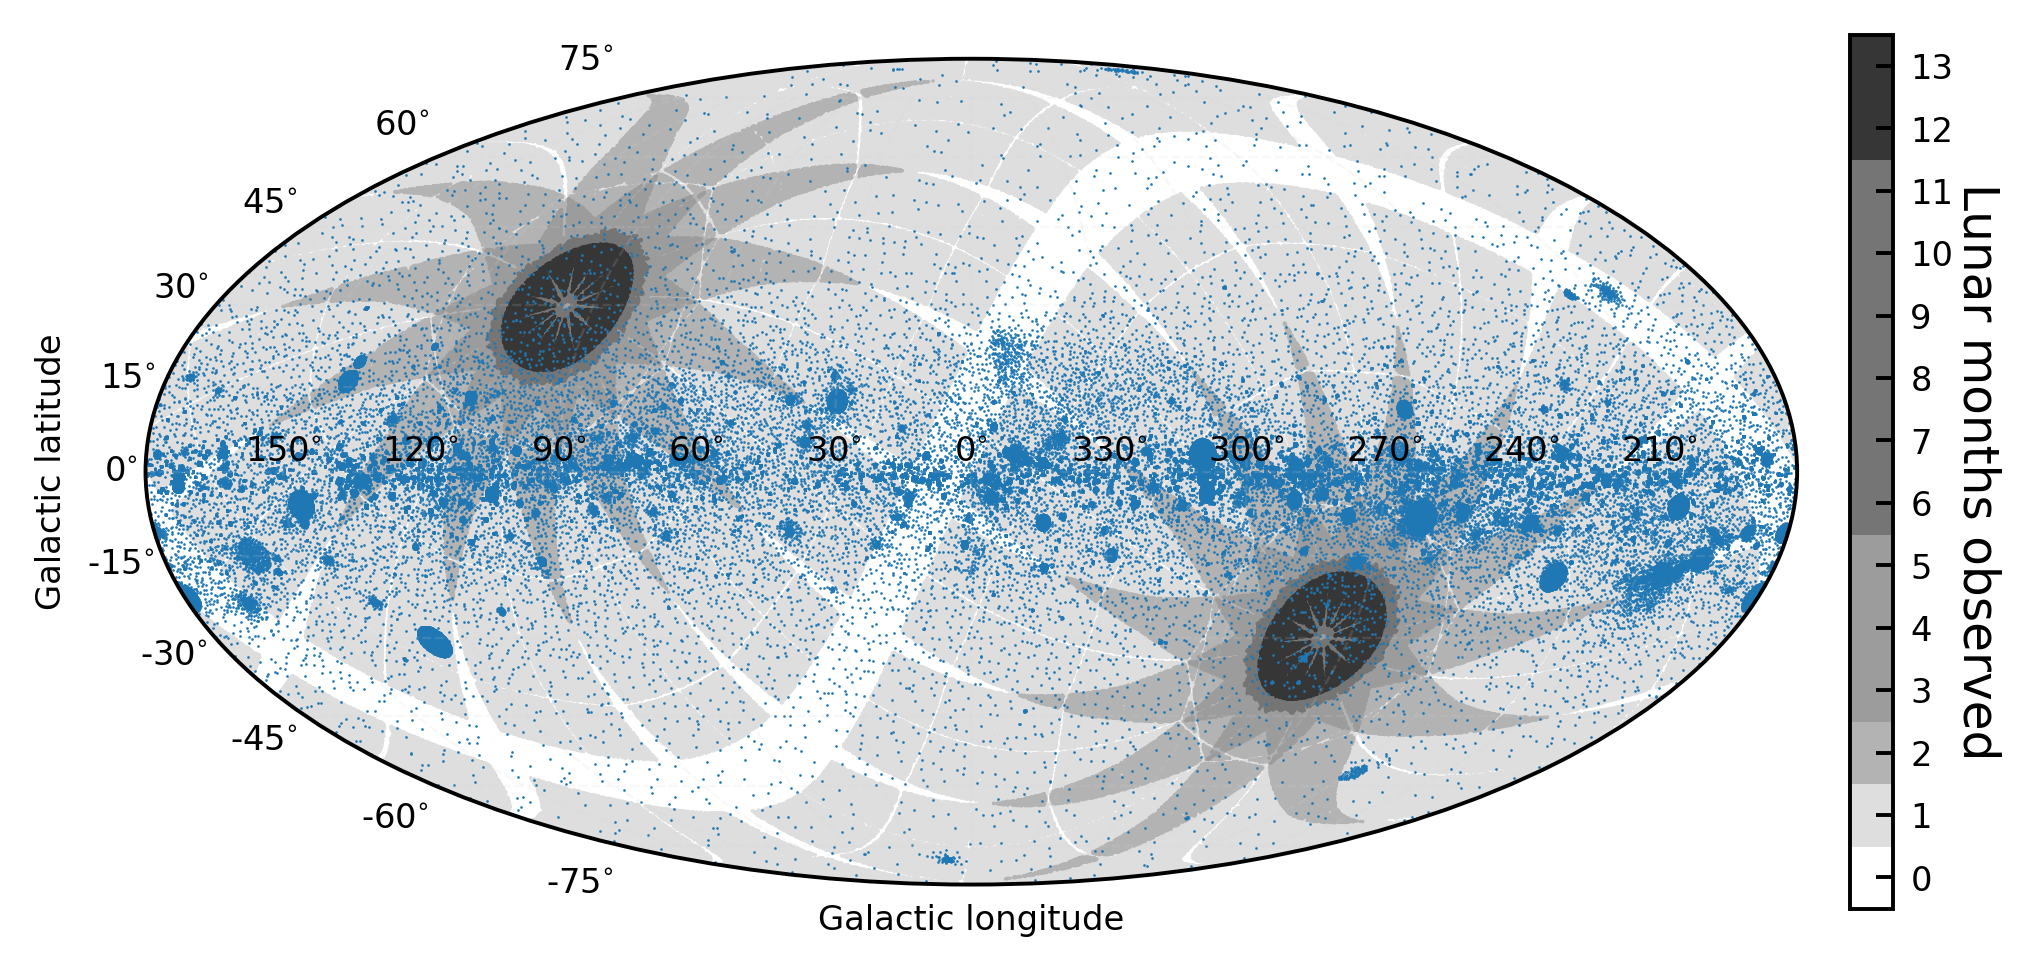
\includegraphics[width=0.9\textwidth]{target_star_positions.png}
		%\gridline{\fig{target_star_cumulative_counts.pdf}{0.41\textwidth}{}}
	\end{center}
	\vspace{-0.8cm}
	\caption{
    Target star positions (blue) and predicted TESS
    observing footprint (gray).
    Target stars are either candidate members of clusters, or
    else have other youth indicators (see \S~\ref{sec:starselection}).
    Most will be observed for one or two lunar months over the course
    of the TESS Prime Mission.
    \label{fig:cdips_targets_positions}
	}
\end{figure*}

\begin{figure}[!t]
	\begin{center}
		\leavevmode
		%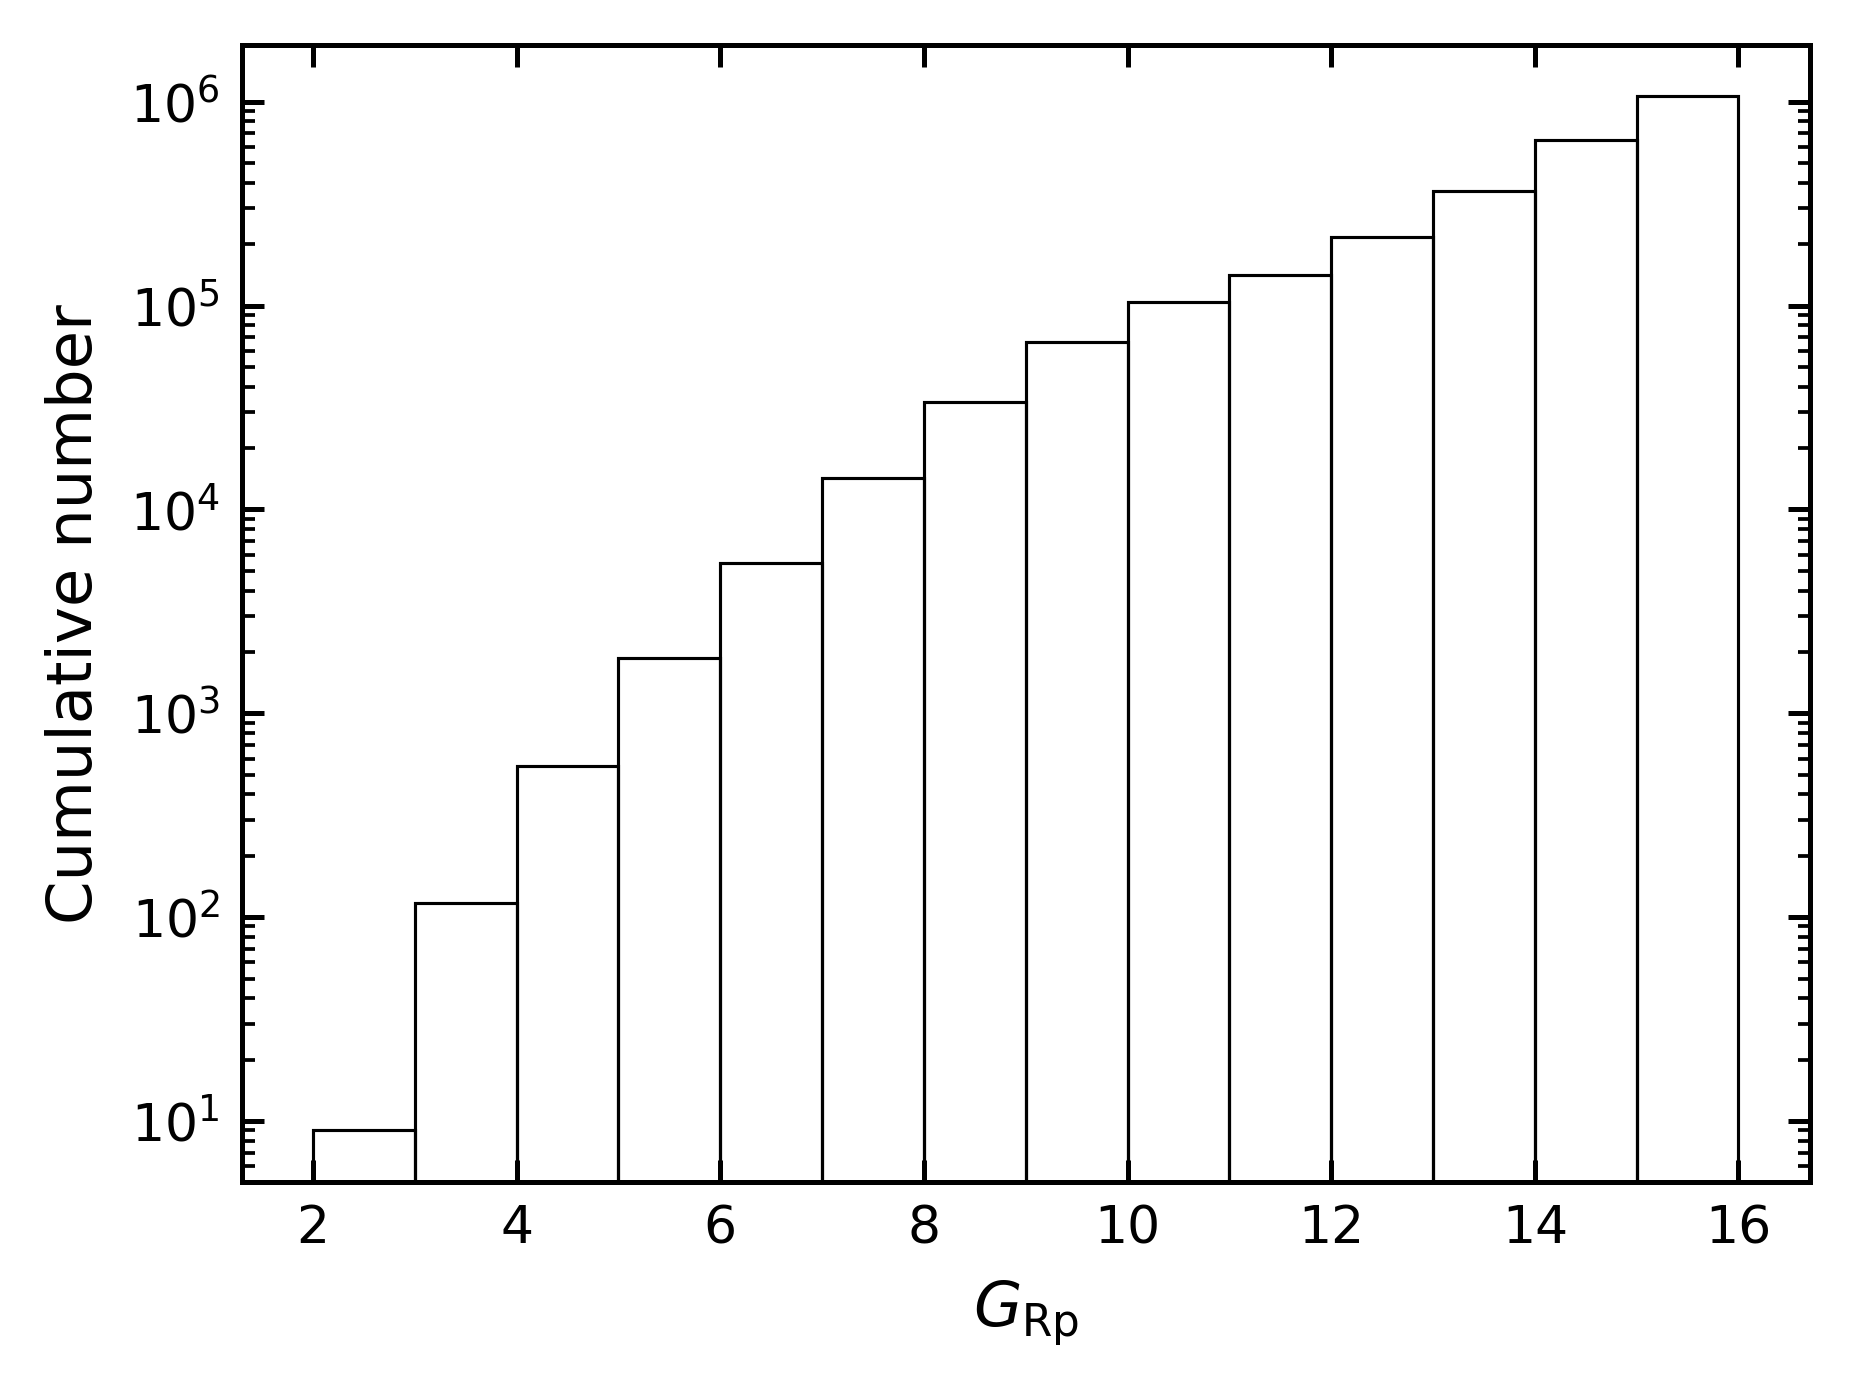
\includegraphics[width=0.45\textwidth]{target_star_cumulative_counts.png}
		\gridline{\fig{target_star_cumulative_counts.pdf}{0.41\textwidth}{}}
		\vspace{-0.8cm}
		\gridline{\fig{target_star_hist_logt.pdf}{0.41\textwidth}{}}
		\vspace{-0.8cm}
		\gridline{\fig{target_star_reference_pie_chart.pdf}{0.41\textwidth}{}}
	\end{center}
	\vspace{-0.8cm}
	\caption{
		Target star statistics.
		{\it Top.} Cumulative counts as a function of Gaia $Rp$-band
		magnitude.  
		{\it Middle.} Histogram of target star ages, for the subset of
		stars with ages matched against \citet{Kharchenko_et_al_2013}.
		{\it Bottom.} Provenance of cluster membership.  Percentages are
		relative to $N_{\rm total}=1061446$ target stars. Symbols
		are as follows.
		D14 is \citet{dias_proper_2014}.
		K13 is \citet{Kharchenko_et_al_2013}.
		CG18 is \citet{cantat-gaudin_gaia_2018}.
		Z18 is \citet{zari_3d_2018}, with upper main sequence and
		pre-main-sequence samples sub-divided.
		``$\geq 2$'' indicates at least two authors reported a star as a
		candidate cluster member.
		%``Other'' refers to sources enumerated in \S~\ref{sec:starselection}.
		\label{fig:cdips_targets}
	}
\end{figure}

\begin{figure*}[!t]
	\gridline{\fig{mwscmatchstats.pdf}{0.95\textwidth}{}}
	\vspace{-0.8cm}
	\gridline{\fig{dias14matchstats.pdf}{0.95\textwidth}{}}
	\vspace{-0.8cm}
	\caption{
		{\it Top.} Quality diagnostics from cross-matching
		\cite{Kharchenko_et_al_2013} cluster members against Gaia-DR2.
		histogram of the distances between matched stars is on the left; a
		histogram of the difference between the true $G$-band magnitude
		and that predicted from 2MASS photometry is in the middle; a scatter
		plot of the same magnitude difference as a function of $G$-band
		magnitude is on the right.
		{\it Bottom.} Same, but cross-matching \cite{dias_proper_2014}
		cluster members to Gaia-DR2.
	}
	\label{fig:xmatch_info}
\end{figure*}

The main aim of the CDIPS project is to increase the number of cluster
stars for which photometric time-series are available, and thereby
facilitate studies of exoplanetary and stellar processes across
different times and stellar environments.  An essential step is
therefore to define a sample of stars that are thought to be young, or
members or clusters, or both.

A homogeneous membership calculation for every known cluster is a
rather large undertaking, and currently falls outside our scope.  So
too is a homogeneous search for young stars across the galaxy.
Instead, we have opted to collect and concatenate appropriate catalogs
from across the literature.  We then use the resulting meta-catalog to
identify our target stars within the TESS images.

The probabilistic criteria for inclusion in our target star list is
necessarily heterogeneous across different catalogs.  However, in our
initial stellar selection our aim is completeness, not accuracy.  If
there has been a claim in the literature that a star should be
considered a cluster member, or a young star, we would like to err on
the side of reporting a light curve for the star.  For stars that are
photometrically interesting, we can then perform post-hoc quality
checks using Gaia-DR2 astrometry and photometry to assess cluster
membership and youth.

\S~\ref{subsec:oc} describes the catalogs we used to identify
candidate members of open clusters.  \S~\ref{subsec:mg} describes the
catalogs we used to identify candidate members of moving groups,
stellar associations, as well as young stars identified through
combined Gaia photometry and astrometry.  \S~\ref{subsec:ocmgsummary}
and Figure~\ref{fig:cdips_targets} describe summary statistics for the
entire sample of about one million target stars.

%FIXME: make table

\subsection{Big catalogs: open clusters}
\label{subsec:oc}

At the time of writing, two relatively large, homogeneous cluster
memberships studies had been performed using {\it Gaia}-DR2: those by
\citet{cantat-gaudin_gaia_2018} and \citet{gaia_hr_2018}.
There were also two large membership studies based on proper motion and 
photometric catalogs that were of interest: the studies of
\citet{Kharchenko_et_al_2013} and \citet{dias_proper_2014}.

\paragraph{{\it Gaia}-derived OC memberships}

\citet{cantat-gaudin_gaia_2018} used the UPMASK unsupervised membership
assignment algorithm \citep{krone-martins_upmask_2014} to identify cluster
members using Gaia-DR2 positions, proper motions, and parallaxes.
They used {\it Gaia} photometry and radial velocities to then verify the
claimed membership properties.  From their Table~2, we collect an initial
401{,}448 cluster members, in 1229 clusters, down to their limiting magnitude
of $G=18$.

\citet{gaia_hr_2018} reported memberships for stars in a smaller, more
select group of well-studied open clusters. From their Table~A1, we
collect 40{,}903 cluster members, in 41 open clusters, mostly within
$500\,{\rm pc}$. While this work also included memberships for
globular clusters, we omitted these from consideration.

Given the unprecedented quality of Gaia-DR2 astrometry, these two
membership sources are our most reliable sources of membership
information.  In our photometric reduction,  our default identifier
for all sources is correspondingly the Gaia-DR2 \texttt{source\_id}.
The TIC identifiers are found through a spatial cross-match after the
light curves have been made, subject to the requirement that the
Gaia-DR2 source identifiers match
\citep{stassun_TIC_2018,stassun_TIC8_2019}.  

% We take this approach
% because Gaia-DR2 is the base-catalog used to project sources from
% celestial coordinates to the imaging plane (\S~\ref{sec:method}).  It
% also has the advantage that for any Gaia-derived cluster memberships,
% we can cross-match directly against source identifiers.



\paragraph{Pre-{\it Gaia} OC memberships}
\citet{Kharchenko_et_al_2013} used proper motions calculated in PPMXL
\citep[][a combination of USNO-B1{.}0 and 2MASS
astrometry]{roeser_ppmxl_2010} and near-infrared photometry from 2MASS
\citep{skrutskie_tmass_2006} to report the existence of 2859 open
clusters and stellar associations (globular clusters were omitted by
excluding any entry of type \texttt{'g'}).  We selected the most
probable cluster members (``$1\sigma$ members'') using the combined
photometric, kinematic, and spatial criteria described by
\citet[][Section~3.3]{kharchenko_global_2012}.  Then, to obtain {\it
Gaia}-DR2 source identifiers for the members, we performed a
crossmatch for {\it Gaia}-DR2 sources within 5 arcseconds of the
listed positions.  To improve the quality of the cross-match, we
additionally used the 2MASS photometry to predict the $G$-band
magnitudes\footnote{See
\url{https://gea.esac.esa.int/archive/documentation/GDR2/Data_processing/chap_cu5pho/sec_cu5pho_calibr/ssec_cu5pho_PhotTransf.html},
online, \texttt{2019-03-29}, or \citet{carrasco_gaia_2016}}, and
required that the measured $G$-magnitude fall within 2 magnitudes of
the predicted $G$-magnitude.  If multiple neighbors matched the
position and magnitude constraints, we took the nearest spatial
neighbor as the match.  From 373{,}226 stars, this yielded a unique
best neighbor for 352{,}332 stars (94.4\% of the sample), and a choice
between two neighbors for 17{,}774 stars. 

%FIXME is this it?
The second (non-{\it Gaia} derived) open cluster membership catalog we
used was the \citet{dias_proper_2014} catalog, which was based on
UCAC4 proper motions acquired by the US Naval Observatory
\citep{zacharias_fourth_2013}.
From their 1805 reported open clusters, we selected sources with
quoted membership probability above 50\%.
To obtain {\it Gaia}-DR2 source identifiers for the members, we
performed a similar crossmatch as before, looking for sources within 5
arcseconds of the listed positions, and within $\pm$2 $G$-band
magnitudes of the prediction.
From 2{,}034{,}269 stars, this yielded a unique
best neighbor for 1{,}828{,}630 stars (89.9\% of the sample), and a choice
between two neighbors for 8.7\% of the remaining sample. 

The distributions of various cross-matching statistics are shown in
Figure~\ref{fig:xmatch_info}.  The distances between matches is
typically below 1 arcsecond.  The Dias catalog shows somewhat stronger
crowding effects at the faint end compared to the Kharchenko catalog,
and likely has a larger number of false matches.
At their faint ends, both catalogs show a tendency for true $G$-band
magnitudes being somewhat larger than predicted $G$-band magnitudes,
due to dust reddening.


\subsection{Smaller catalogs: moving groups and stellar associations}
\label{subsec:mg}

Stars, moving groups and stellar associations are of interest for
similar reasons as stars in open clusters.  Though fewer stars
are known to exist in moving groups, they are of particular interest
because moving groups are less crowded than open clusters, and are
often closer to the Sun.

We obtained Gaia-DR2 identifiers from the results of the following
studies:
\citet{gagne_banyan_XI_2018},
\citet{gagne_banyan_XII_2018},
\citet{gagne_banyan_XIII_2018},
\citet{kraus_tucanahor_2014},
\citet{roser_deep_2011}, % OC, not MG...
\citet{bell_32ori_2017},
\citet{rizzuto_multidimensional_2011},
\citet{oh_comoving_2017}, and
\citet{zari_3d_2018}. The methods applied in these studies
vary from kinematic analyses, to astrometric analyses included
Gaia-DR1 parallaxes, to photometric searches for infrared excesses, to
spectroscopic studies including RVs, H$\alpha$
emission, and Li absorption.

For the Gagn\'e et al{.} catalogs, we searched the Gaia-DR2 archive for
sources within 10 arcseconds of the listed positions.  If Gagn\'e et
al{.} gave a proper motion, we required that the sign of each the Gaia
proper motion components match that of the Gagn\'e values (the stated
proper motion uncertainties seemed to have been underestimated).  We
also imposed a $G<18$ cut on any putative matches.  Of 3012 moving
group members collected from the three combined Gagn\'e et al{.}
catalogs, we found 2702 matches.

The \citet{kraus_tucanahor_2014}, \citet{roser_deep_2011}, and
\citet{bell_32ori_2017} studies reported members in Tucana-Horologium,
the Hyades, and 32$\,$Ori respectively.  Applying the same procedure as
for the Gagn\'e catalogs gave 187, 684, and 119 best-neighbors
respectively, compared to 205, 724, and 141 initially reported
members.  Note that \citet{kraus_tucanahor_2014} found that only
$\sim$70\% of their listed members have spectroscopic indicators
consistent with their membership in Tucana-Horologium.

\citet{rizzuto_multidimensional_2011} also focused on a single moving
group: the Sco OB2 association. We used their reported Hipparcos
identifiers, and matched against the {\it Gaia} archive's
\texttt{hipparcos2\_best\_neighbour} table, which gave 319
nearest-neigbor stars from 436 candidate members.

Next, \citet{oh_comoving_2017} searched for comoving stars in the
$\approx$2 million stars that overlapped between Tycho-2 and {\it
Gaia}-DR1.  They found many wide binaries, and also identified a large
number of comoving groups.  We chose the 2{,}134 stars that they
reported were in groups with sizes of at least 3 stars.  Using their
{\it Gaia}-DR1 source identifiers, we matched against the {\it Gaia}
archive's \texttt{dr1\_neighbourhood} table, which gave 1{,}881
nearest-neigbor stars in groups of at least three stars
\citep{marrese_gaia_2019}.

Finally, \citet{zari_3d_2018} constructed a sample of young stars
within $500\,{\rm pc}$ using data from Gaia-DR2. Two subsamples were
made: (a) an upper main sequence (MS) sample, with 86{,}102 stars, and
(b) a pre-MS sample, with 43{,}719 stars.  Each was created from a
careful combination of distinct astrometric and photometric cuts.
These stars are the youngest, closest stars, spread across
star-forming complexes in Sco-Cen, Orion, Vela, Taurus, and other
regions of the sky.  Though many are not strictly identified with
moving groups or open clusters, their reported youth and proximity to star
forming regions justifies their inclusion in our search sample.




\subsection{Summary of target stars}
\label{subsec:ocmgsummary}


After collecting the aforementioned lists, we merged them into a
single table. We queried the \texttt{gaiadr2.gaia\_source} table to
retrieve their photometric $G$, $G_{\rm Rp}$, and $G_{\rm Bp}$
magnitudes, as well as their astrometric measurements $(\alpha,
\delta, \mu_\alpha, \mu_\delta, \pi)$.  Finally, we required that
$G_{\rm Rp} < 16$, which is roughly where the 1-hour photometric
precision of TESS is predicted to reach 1\%
\citep{ricker_transiting_2015}.

All told, this procedure yielded 1{,}061{,}447 unique stars, from 13
distinct membership catalogs.

The relative fractions of stars from each catalog are shown in
Figure~\ref{fig:cdips_targets}.
The largest number of stars come from \citealt{dias_proper_2014}
(44.3\% of stars), \citealt{Kharchenko_et_al_2013} (17.3\%),
\citealt{cantat-gaudin_gaia_2018} (16.7\%), and \citealt{zari_3d_2018}
(11.1\%, of which 7.8\% are OBA stars, and 3.3\% are pre-MS stars).
107{,}647 of the stars, or about 10\%
of the collection, have cluster memberships reported by multiple
authors.  Since the membership probability calculations often use
independent data and methods, agreement between multiple investigators
on a given star's cluster membership is a helpful indication of it
being a bonafide member.
Stars reported in multiple catalogs have all available reference information
concatenated.  

The fraction of target stars from each catalog which are bonafide
cluster members should be understood to be heterogeneous.  For the
\citet{dias_proper_2014} catalog, their membership calculation
included only spatial and kinematic information, and we used a
relatively low probability threshold when including their stars (based
on the criteria \citealt{dias_proper_2014} used for their star
counts).  The \citet{Kharchenko_et_al_2013} catalog combined spatial,
kinematic, and photometric information to derive their membership
probabilities.  We also used a somewhat more restrictive membership
probability cut (again, following the criteria they used for their
star counts), and so this sub-sample is likely less contaminated
with field interlopers.
\citet{cantat-gaudin_gaia_2018} used spatial, kinematic, and
astrometric information from Gaia-DR2. Despite the lack of
photometric information, the quality of the Gaia data suggest that the
field contamination rate will be lowest for the
\citet{cantat-gaudin_gaia_2018} sample.


To assign unique cluster names, we adopted the name matched against
\citet{Kharchenko_et_al_2013} whenever possible.
Appendix~\ref{appendix:uniquenames} describes  how this was done in detail.
For moving groups not identified in \citet{Kharchenko_et_al_2013}, we used
the constellation-based naming convention from
\citet{gagne_banyan_XI_2018}.  Otherwise, we used the name reported by
the original catalog claiming membership.  This process reduced 16,425
name permutations down to 3,216 unique cluster names.  Though we have
made every effort to avoid duplicates, a small number may remain, so we
advise inspection of the \texttt{cluster} column
as well as the references given in the
\texttt{reference} column rather than using the
\texttt{unique\_cluster\_name} column to analyze individual objects
of interest.  Nonetheless, 87.7\% of the $\sim$million unique target
stars are matched to clusters within \citet{Kharchenko_et_al_2013},
and 88.8\% are assigned a cluster name.  The remainder are mostly the
young stars from \citet{zari_3d_2018}.
Ages and their uncertainties are then merged against the 
parameters reported by \citet{Kharchenko_et_al_2013}.

The resulting CDIPS target star list is given in Table~N.
The cumulative distribution of target star brightnesses, as well as a
histogram of the ages, is shown in Figure~\ref{fig:cdips_targets}.
Relative to field stars, our target star sample is young, with a
typical age of 100$\,$Myr.






%%%%%%%%%%%%%%%%%%%%%%%%%%%%%%%%%%%%%%%%%%
\section{Method: Photometry}
\label{sec:method}

\begin{figure}[t]
	\begin{center}
		\leavevmode
		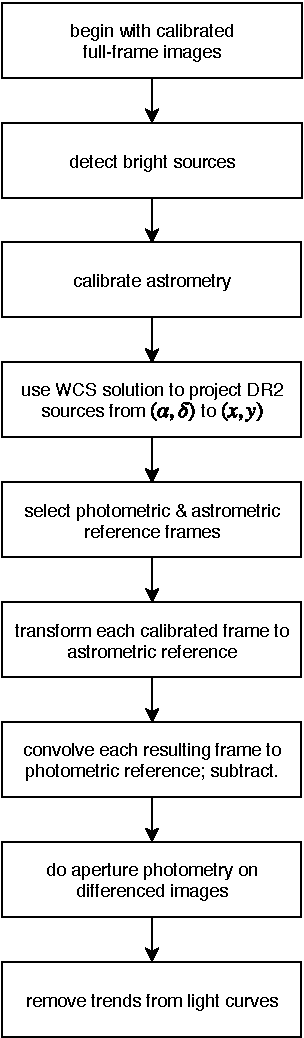
\includegraphics[width=0.3\textwidth]{pipelineoverview.pdf}
	\end{center}
	\vspace{-0.2cm}
	\caption{
    Conceptual overview of photometric reduction pipeline.
    Details are given in \S~\ref{sec:method}.
    %TODO: add latex section numbers!
    %TODO: do FORCED aperture photomery on differenced images
    %TODO: improve text generally
	\label{fig:pipeline}
	}
\end{figure}

\subsection{Overview}

To reduce the TESS images to light curves, we adopted an image
subtraction approach.  The overall method is in the spirit of the
reduction pipelines developed by \citet{Pal_2009},
\citet{huang_high-precision_2015}, \citet{soares-furtado_image_2017}
and \citet{oelkers_precision_2018}; a conceptual overview is given in
Figure~\ref{fig:pipeline}.  Most sub-modules of our pipeline have been
developed over the past decade to process HAT data \citep[{\it
e.g.},][]{bakos_hat_review_2018}.  The specific high-level framework
used for this reduction was adapted from a pipeline called
\texttt{pipe-trex}, under development primarily for the HATPI project
(\url{hatpi.org}).  The code is available
online\footnote{\url{github.com/waqasbhatti/pipe-trex}, commit
\texttt{cd9f9bb}.}.

We begin our processing with the calibrated full frame images produced
by the Science Processing Operations Center at NASA Ames
(\S~\ref{subsec:observations}).  We then perform a collection of
preparatory steps, including source extraction of bright stars,
astrometric verification, and coarse simple aperture photometry of
bright stars (\S~\ref{subsec:preparation}).  Using the information
collected from these initial steps, we select an astrometric reference
frame to which we transform all of the calibrated images.  We
construct a photometric reference by stacking a subset of these
transformed frames, after having convolved the frames to have
identical stellar profiles. Finally, we subtract each target frame
from the photometric reference (\S~\ref{subsec:imagesubtraction}).  We
perform aperture photometry on the subtracted images using positions
projected onto the frame from the Gaia-DR2 source catalog.  We detrend
the resulting light curves (\S~\ref{subsec:lcdetrending}).  The
resulting white noise and red noise properties of the light curves,
and a few interesting cases of variability, are discussed in
\S~\ref{sec:results}.


\subsection{Observations}
\label{subsec:observations}

% How did TESS observe?
% What processing steps happened in order to get the calibrated frames?
% Why did we choose to start with them?

The TESS spacecraft began science operations on July 25, 2018.  To
keep its cameras pointed opposite the Sun, the spacecraft advances by
$\approx$$28$ degrees east in ecliptic longitude every lunar month.
Data acquired throughout each ``sector'' are downlinked at spacecraft
perigee through the Deep Space Network.  Descriptions of the
spacecraft's design and operations are given by
\citet{ricker_transiting_2015} and the instrument handbook
\citep{vanderspek_2018}.

For us, the main data product of interest is the calibrated full frame
image (FFI).  Each TESS camera is read out every 2 seconds.  To
produce a manageable telemetric load, the resulting pixel values are
averaged by the onboard computer into 30 minute exposures. An on-board
cosmic ray mitigation algorithm is applied \citep[][\S
5.1]{vanderspek_2018}. Once transmitted to the ground, the raw images
are calibrated by the Science Processing Operations Center (SPOC).  The
calibration process includes an overscan, bias, and dark current
correction, and also divides out a flat field.  Details are discussed
by \citet{clarke_kepler_2017}, and the resulting science data products
are described by \citet{tess_data_product_description_2018}.

We perform our processing using the calibrated images, their
corresponding uncertainty images, and the associated headers.  The
spacecraft has four cameras, and each camera has four CCDs.  In the
following analysis, all image-level operations are thus performed on
the images for each CCD, so that at any instant of time there are 16
independent images that require analysis.

While we performed numerous initial tests on the first sectors of
data, by geometric coincidence Sectors 1--5 were pointed away from the
galactic plane.  Consequently, less than 2\% of the CDIPS target star
sample was observed in the first five TESS sectors.  Though a few
interesting clusters are present in these observations ({\it e.g.},
Blanco~1, NGC~2516, NGC~1901), for the present work we opted to focus
on sectors in which there were more stars of interest for our intended
science.  These begin in Sector 6 (2018-12-12, spacecraft orbit \#19).
For this run of processing, they conclude at the end of Sector 7
(2019-02-01, spacecraft orbit \#22).
Sectors 6 and 7 cover galactic longitudes from roughly 200$^\circ$ to 280$^\circ$, 
with fair coverage within $\pm 20^\circ$ of the galactic plane
(Figure~\ref{fig:cdips_targets_positions}).


\subsection{Image preparation \& background removal}
\label{subsec:preparation}

Before we can perform any kind of photometry, a few janitorial tasks
are required.
First, we convert the multi-extension calibrated FITS image from MAST
into a single-extension FITS image, and trim to remove virtual rows
and columns using the \texttt{SCIROWS}, \texttt{SCIROWE},
\texttt{SCCSA}, and \texttt{SCCED} header values.

In order to pre-emptively address the background variations present in
some frames due to scattered light from the Earth and Moon
\citep[see][\S 7.3.1--7.3.4]{vanderspek_2018}, we then estimate and
subtract the large-scale background.  We do this by temporarily
masking out pixels more than $2\sigma$ from the image median, and then
pass a $48\times48$ median box filter over each pixel in the image,
with reflective boundary conditions.  The resulting background
estimate has low-amplitude structure over spatial scales of a few
pixels, so we then blur it with a gaussian kernel to produce a smooth
background estimate for each image.  These steps also remove a
low-level vignetting present in the corners of many images, which
remains even after flat-fielding \citep[see][\S
7.3.5]{vanderspek_2018}.  With the exception of scattered light
patches, which remain over small areas of less than 10\% of the
frames, our ad-hoc procedure seems to adequately remove large spatial
scale scattered light patches.

% We found this background subtraction step to be particularly important
% in our subsequent difference imaging analysis. In its absense, the
% scattered light artifacts could introduce erroneous residuals into the
% kernel solution used to match reference and target images.  Including
% this step mitigated such effects, and helped produce clean
% subtractions.  Even after subtraction, a small fraction of frames also
% show sharp features (caustics) below our median box filter's size
% scale.  Such features may affect flux measurements at specific times
% in a small subset of light curves.

After subtracting the background, we mask out saturated pixels using a
fixed saturation level of $8\times10^4\,{\rm ADU}$. This value was
chosen based on the onset of bleeding charge trails in the images, and
is slightly greater than the saturation level of $2\times10^5$
electrons, or about $4\times10^4\,{\rm ADU}$, quoted by
\citet{vanderspek_2018}. 
We correspondingly do not analyze stars brighter than $T\approx 6.5$.
As described by \citet{Pal_2009}, the pixel masks are metadata to the
image, and are only applied to the pixel values during the specific
image processing steps in which they are necessary ({\it e.g.},
convolution). We also extend the masks beyond purely saturated pixels
to ``bloomed'' pixels horizontally and vertically adjacent to the
saturated pixels (see Figure~6 of \citealt{Pal_2009}).

Finally, for frames with the \texttt{DQUALITY} bit-flag corresponding
to the ``momentum dumps'' and ``coarse pointing modes'' described by
\citet{vanderspek_2018}, we omit the entire frame.  This removes on
average a few frames per sector, out of about one thousand. Through
visual inspection, we see that the stars on these frames are extremely
smeared, and are unlikely to produce useful science data.  In
addition, we use the sector-specific data release notes\footnote{\url{
  archive.stsci.edu/tess/tess_drn.html}} to identify further times
with anomalous spacecraft performance, which we omit from
consideration.  For Sectors 6 and 7, this included three days at the
beginning of Sector 6 dedicated to acquiring pixel response function
data, and no additional gaps in Sector 7.
%For Sectors 1 through 5, these
%include coarse pointing windows from orbits 10, 13, 14, and an
%instrumetal anomaly window in orbit 15.
% For Sectors 6 through 8, these include three days at the beginning of
% Sector 6 dedicated to acquiring pixel response function data, and also
% about three days during Sector 8 lost to an instrument anomaly.

\subsection{Metadata collection \& WCS verification}
\label{subsec:metadatacollection}

\begin{figure}[!t]
	\gridline{\fig{astromresidual_hist.pdf}{0.5\textwidth}{}}
	\vspace{-0.8cm}
	\gridline{\fig{astromresidual_quiver.pdf}{0.5\textwidth}{}}
  %\vspace{-0.8cm}
	%\gridline{\fig{astromresidual_apertures.pdf}{0.5\textwidth}{}}
	\vspace{-0.8cm}
    \caption{
		{\it Top.} Histogram of astrometric residual. The $x$-axis shows 
		the distance between the measured centroid positions of stars, 
		compared to the predicted positions from the WCS solution.
		{\it Bottom.} Vector plot of astrometric residual. Each arrow is 
		the vector from the measured to the projected star position. 
		Directions are correct, but lengths are 50 times their true size for 
		visualization purposes.
    The systematic error in the top-right corner is a typical
    problem generic to wide-field astrometry.
    The frame chosen for this plot is the photometric reference frame used 
    for Sector 6, Camera 1, CCD 1; we automatically 
    impose cutoffs on the median and $90^{\rm th}$ percentile of the 
    astrometric residual in order to ensure similar levels of astrometric 
    precision are maintained throughout the reduction.
	}
	\label{fig:astromresid}
\end{figure}

Having prepared the images, we perform some initial analysis steps to
produce metadata needed during image subtraction.  

First, we use \texttt{fistar} to perform source extraction on the
thousand or so brightest, non-saturated stars in each image.  The
source extraction derives centroid positions for these stars, and also
fits elongated gaussians to their profiles, yielding the shape
parameters $(s,d,k)$, where the flux $f$ as a function of position
$(x,y)$ in the CCD image plane is assumed to take the form
\begin{align}
  f(x,y) &= B + A \exp \{ -0.5 \times [
    s(\Delta x^2 + \Delta y^2) + \\
    \nonumber
    &d(\Delta x^2 - \Delta y^2) +
    k(2\Delta x \Delta y)
  ]  \},
\end{align}
for $(x_0,y_0)$ arbitrary reference positions,
$\Delta x = x-x_0$, $\Delta y = y - y_0$, $B$ is the background
level, and $A$ is an arbitrary
flux-scaling constant.
For a nearly circular shape profile, the sharpness $s$ is related to
the FWHM as ${\rm FWHM} \approx 2.35\sqrt{s}$ \citep[{\it
e.g.},][]{Pal_2009}.  These shape parameters are later used when
selecting an astrometric reference frame
(\S~\ref{subsec:imagesubtraction}).  
In agreement with what is obvious upon visual inspection, this 
fitting process shows that stars closer to the
center of each camera's field are round, while
stars near the field edges are more triangular.

For the astrometric solution, we use the World Coordinate System (WCS)
and fourth-order Simple Imaging Polynomial (SIP) coefficients
derived by SPOC and included in the FFI headers
\citep[][Sec.~8]{pence_fits_2010}.  We explored the possibility of
using \texttt{astrometry.net} \citep{lang_2010} to derive our own
astrometric solutions for each frame, but found that the astrometric
residual (the mean separation between projected and measured
positions) was consistently a factor of 1.5-2 times higher in our WCS
solutions than in those given by SPOC.  This was perhaps because
we did not invest major amounts of time developing a robust
algorithm to select non-blended stars of intermediate brightness before
measuring their positions.

With the resulting WCS information, we then project a source catalog
onto each frame.  Initially, we planned to photometer all Gaia-DR2
sources in each field down to a cutoff of $G_{Rp} < 16$.  However, we
found that for the galactic plane fields this produces an excessively
large number of sources (millions of stars per
$12^\circ\times12^\circ$ CCD).  We therefore limited our source
catalog for each frame to be
a combination of the CDIPS target stars ($G_{Rp} < 16$), and
all Gaia-DR2 sources down to $G_{Rp} < 13$.  We use the
projected positions of these sources to center the apertures in our
photometry,
rather than attempting to detect the positions.  Such
``forced-aperture photometry'' is preferable to source
extraction in the crowded fields that are central to this work.  The
Gaia-DR2 epoch is J2015.5, so even the fastest-moving stars with
proper motions of $\sim$$1\,{\rm arcsecond}\,{\rm yr}^{-1}$ are still
well within one pixel of their predicted positions in the TESS images.
The projection from catalog sky-coordinate positions to pixel
coordinates is performed using an analog of the \texttt{wcs-rd2xy}
program that performs the standard matrix algebra \citep{lang_2010}.
The source catalog look-up is performed using
\texttt{gaia2read}\footnote{\url{github.com/samuelyeewl/gaia2read}}
\citep{kim_2018_gaia2read}.

The residual between the measured and projected stellar centroid
positions is displayed for one photometric reference frame in
Figure~\ref{fig:astromresid}.
The construction of this frame will be described shortly, however
a few salient points can first be made.
First, the typical median precision of the WCS solution is a bit below
0.1 pixels, and its $90^{\rm th}$ percentile is typically less than
0.3 pixels\footnote{In fact, in our reduction we automatically impose
that the median residual and 90th percentile remain below 0.2 and 0.4
pixels, respectively.}.
%The distribution has a outlier tail of saturated stars which were
%masked, and thus do not have measureable centroid positions.
The errors are typically largest in the corners of the field of view,
where the non-linearity of the focal plane is most significant, and
where the corrections required by the SIP coefficients are largest.
%The final sub-panel of Figure~\ref{fig:astrometricresidual} is a
%sanity check on the location of the projected positions, and also
%gives some context for our chosen aperture radii of 1, 1.5, and 2.25
%pixels.

As a final step of metadata collection, we perform aperture photometry on the
bright stars by summing the counts inside appropriately-weighted
circular apertures centered on the projected positions. This task is
performed using \texttt{fiphot}.
The pixel weights are equal to the fraction of the pixel
that falls within the aperture.  They are thus unity for pixels
entirely within the aperture, and fractional along the aperture
boundary. % (see \citealt{Pal_2009} Fig 17). 
The background levels are measured in annuli around each aperture
center. 
%The raw flux of the object after background removal is then
%(\citealt{Pal_2009} Eq 65)
%\begin{equation}
%  f = \sum_{x,y} w_{x,y} (I_{x,y} - B) = f_{\rm total} - B r_0^2.
%  \label{eq:simple_aperture_phot}
%\end{equation}
The resulting measurements, for instance of the background level of
each aperture, and the number of stars with ``good'' photometry,
are later used to select photometric reference frames.


\subsection{Image subtraction}
\label{subsec:imagesubtraction}

\subsubsection{History of image subtraction method}
The core operation of ``classical'' image subtraction
attempts to match a photometric reference $R$ and a target image $I$ by 
computing and applying a convolution kernel.
For ground-based data, this ``match'' typically corrects for
differences in seeing or transparency between the reference and
target; for space-based data, the match might correct for spacecraft
jitter, or thermal and corresponding point-spread function (PSF)
variations.
The kernel, once applied to the high signal-to noise reference,
produces a model image, $M_{xy}$,
\begin{equation}
    M_{xy} = (R \otimes K)_{xy} + B_{xy},
    \label{eq:imagemodel}
\end{equation}
where $B_{xy}$ is a component of the model image that allows for
background variations, and $\otimes$ denotes convolution.
Since we modeled the background separately (\S~\ref{subsec:preparation}),
we set $B_{xy}=0$.
The convolution kernel $K$ is typically decomposed onto a
basis, $K = \sum_i c_i K_i$, and the coefficients are found
by minimizing
\begin{equation}
    \chi^2 = \sum_{xy} \left( \frac{I_{xy} - M_{xy}}{\sigma_{xy}} \right)^2,
    \label{eq:chisq_conv}
\end{equation}
where $\sigma_{xy}$ is the uncertainty in the target image pixel values.
Photometry is then performed on the difference image $D_{xy}$, where
$D_{xy} = I_{xy} - M_{xy}$.
For the present reduction, the uncertainty in each target image pixel was
taken to be a constant.	

The procedure described above was first proposed by \citet{Alard_Lupton_1998}.
It was reviewed and clarified by \citet{miller_optimal_2008}.
The choice of how to decompose the kernel was further explored by
\citet{bramich_new_2008}, who showed that using a linear combination
of delta functions had advantages compared to a basis of gaussians.
We perform the convolution using \texttt{ficonv}, and opt for the
implementation of Bramich's method (see \citealt{Pal_2009} \S~2.8).


\subsubsection{Astrometric registration}
We now describe a few implementation details we used to make the
above high-level picture work.
First, we needed to select two ``reference frames'' for image subtraction:
(1) the astrometric reference; and (2) the photometric reference.

To choose the astrometric reference, we searched for frames with
large, round stars (big $s$, small $d$ and $k$ values).
We also required
that the frame have minimal background noise, as measured in annuli
around the bright stars selected in \S~\ref{subsec:preparation}.
Finally, the astrometric reference frame needed to have, relative to the 
other frames being
considered, a large number of detected sources.
We sorted the frames using these metrics, and then selected the
astrometric reference from successive intersections of each sorted
list.

We then
used the \texttt{grmatch} and \texttt{grtrans} tools to
compute and apply a spatial transformation of each calibrated frame
to match the astrometric reference frame.
The transformation is calculated using the measured source positions
found in ~\S~\ref{subsec:metadatacollection},
and the symmetric triangle point-matching scheme described
by \citet[][~\S~2.5.2]{Pal_2009}.
The transformation~--~a combination of rotation, dilation, and
translation~--~typically moves stars by less than a pixel, since
the TESS spacecraft is quite stable.
The precision of the transformation is guaranteed by forcing 
its unitarity $\Lambda$ to always be below 0.01, where 
$\Lambda$ is defined by \citet[][~Eq.~54]{Pal_2009}.
We reduced the photometric errors
incurred during this step by using
the flux-conserving interpolation
scheme described by \citet{Pal_2009},
which was necessary because polynomial interpolation schemes
do not conserve stellar flux. 

\subsubsection{Photometric reference frame construction \& reference flux measurement}

The second required reference frame is the
photometric reference, which is used both to calculate the
convolution kernel, and to obtain a
reference flux for each star.  
To make it, we first chose 50
sub-frames with low scatter in their photometry
and low background measurements, according to the metadata collected
in \S~\ref{subsec:preparation}.
We then convolved these candidate photometric reference frame to the best
frame, and performed a median average over the entire stack
to make the photometric reference.

%\begin{enumerate}
%  \item Lowest median scatter in photometry
%  \item Lowest median error in photometry
%  \item Lowest median background measurement
%  \item Lowest median absolute deviation in background measurements
%  \item Largest number of stars detected by \texttt{fiphot} with good
%    flags.
    % fiphot files used for all of this.
%\end{enumerate}

Measuring the reference flux for each star is a slightly non-trivial
operation.
First, we perform forced simple aperture photometry to measure
the flux for each source.
The local background is estimated in annuli, with neighboring stars
masked out during the background measurement.
However if we were to stop here, {\it it would be a bad mistake}.
The reference fluxes for faint stars would be overestimated, due to
crowding.
The relative amplitude of photometric signals would correspondingly
be biased small, hindering exoplanet detection.

Therefore, after performing simple aperture photometry on the 
reference frame, we fitted an aperture-size specific zero point
between the catalog $T$-band magnitude of each star, and its
measured flux.
The $T$-band magnitude was calculated according to Equation~1 of 
\citet{stassun_TIC8_2019}.
We then use the known catalog magnitude to predict the expected
reference flux for each star.
In effect, this minimizes crowding down to Gaia's resolution limit of
$\approx$1$''$, rather than the TESS limit of $\approx$20$''$.

Following \citet{Pal_2009}~Equation~83,
the final instrumental flux values $f$ we report\footnote{For example,
the \texttt{IFL1} column.} are then equal to
\begin{align}
f &=  f_{\rm reference} + f_{\rm subtracted} \\
&=
g \left(T_{\rm cat} \right)
+
\frac{1}{|| K ||_1^2} \sum_{x,y} D_{x,y} (w \otimes K)_{x,y}.
\label{eq:ism_flux_measurement}
\end{align}
The function $g$ takes as input the target star's
catalog magnitude $T_{\rm cat}$, and returns the reference flux.
Its coefficients have been fit per the procedure just discussed,
independently for each aperture.
The difference image $D$ is equal to $I -  R\otimes K$,
where as in Equation~\ref{eq:imagemodel}, $I$ is the target image 
transformed to the astrometric
reference, $R$ is the photometric reference, and $K$ is the convolution
kernel.
The weights $w$ from the circular aperture mask are included in
the convolution.
The norm $|| K ||_1$ is defined by \citet{Pal_2009}~Equation~81.

\subsection{Choice of convolution kernel}
A few brief notes on the algorithm to actually solve for the
coefficients to the convolution kernel.  The procedure implemented in
\texttt{ficonv} is to subdivide the image, and within each grid
element find the brightest non-saturated star. These isolated
``stamp'' stars are then used to solve for the coefficients of the
kernel, by minimizing Equation~\ref{eq:chisq_conv} over the sum of all
stamps.

%NOTE : this is kind of incomprehensible
%CHECK: does the polynomial weighting actually do what you want it to do?
For the choice of basis, we opt for a delta-function kernel with an additive
flux scaling term (\citealt{soares-furtado_image_2017} Section 3.3.1
gives the equations).
The spatial variations of the PSF are captured by weighting the 
delta function and the flux scaling terms with varying
polynomial orders across the image.
Choosing this kernel introduces three additional
free parameters:
(1) the kernel box-size;
(2) the maximum order of the polynomial weighting the delta function terms;
(3) the maximum order of the polynomial weighting the flux scaling.
We performed a grid-search to tune these parameters, in
which our metrics for success included the measured RMS as
a function of magnitude, and also the recovered SNR of transits from
the catalog of known TOIs (TESS Objects of Interest; N.~Guerrero, in prep).

Varying the kernel box-size, we found that kernels with box-length smaller than the 
typical TESS FWHM at field center ($\approx$3 pixels) produced light curves
with the highest average scatter.
Increasing the kernel box-size from a $3\times3$ box to a $7\times7$ box led
to about a 50\% reduction in RMS for bright stars, and no difference for 
faint stars.
The largest kernels, of $(11\times11)$ pixels, had on average slightly lower 
signal-to-noise for recovered transits than for kernels of intermediate size.
We settled on a kernel box-size of $(7\times7)$ pixels, in part because the 
FWHM at the camera corners can grow by factors of $\approx$2 relative to the 
field center.

Varying the polynomial orders, we found that the highest order polynomials 
retrieved transits with $\approx10\%$ worse SNR compared to lower order
polynomials.
Varying the polynomial orders between 1 and 4 did not produce large 
differences.

Averaging over all TOIs present in the camera we used for these experiments, 
we found that different choices 
of kernel parameters produced variations of $\lesssim 12\%$ in the retrieved 
transit SNR.  
For computational expediency, we therefore chose a single
$(7\times 7)$ kernel with 
second-order spatial polynomial weights in the basis functions for the
remainder of our reduction.
However, we caution that within our parameter-tuning experiments, the 
recovered SNR of perhaps a third of the TOIs varied by up to a factor of two,
which in a few 
cases led to non-detections of transit signals near the noise floor.
In the longer term, developing an image-subtraction method that marginalizes 
over uncertainties of how to chose ``optimal'' kernels would be desirable.
Pixel-level image subtraction methods that omit these 
parameters entirely 
are also worth exploring \citep{wang_pixel-level_2017}.

With a kernel selected, and the convolution and subtraction performed, 
we calculate the instrumental fluxes for each frame per 
Equation~\ref{eq:ism_flux_measurement}. 
We did this with three different aperture sizes: for this work, circles
of radii 1 pixel, 1.5 pixels, and 2.25 pixels.
These sizes were chosen to roughly span the range of optimal aperture
sizes for stars in our sample, as calcuated from the pre-flight
\citet{Sullivan_et_al_2015} noise model.
Finally, to convert from a list of 
flux measurements for each source on a frame to a list of flux values
at any given time, we used the 
\texttt{grcollect} transposition tool.

\subsection{Light curve detrending}
\label{subsec:lcdetrending}

\begin{figure*}[!t]
	\gridline{
    \fig{raw_light_curve_systematics_sec6cam1ccd2.pdf}{0.48\textwidth}{}
    \fig{raw_light_curve_systematics_sec7cam2ccd4.pdf}{0.48\textwidth}{}
  }
	\vspace{-0.5cm}
	\caption{
	Twenty randomly selected raw image-subtracted light curves drawn
	from the same sector, camera,
	and CCD, for stars with $T$-band magnitudes between 13 and 14.
	A number of systematic trends are shared across the light curves.
	The sector, camera, and CCD numbers are 6, 1, 2 (left) and 7, 2, 4 (right).
	\label{fig:lc_systematics}
	}
\end{figure*}

\begin{figure}[!t]
	\begin{center}
		\leavevmode
		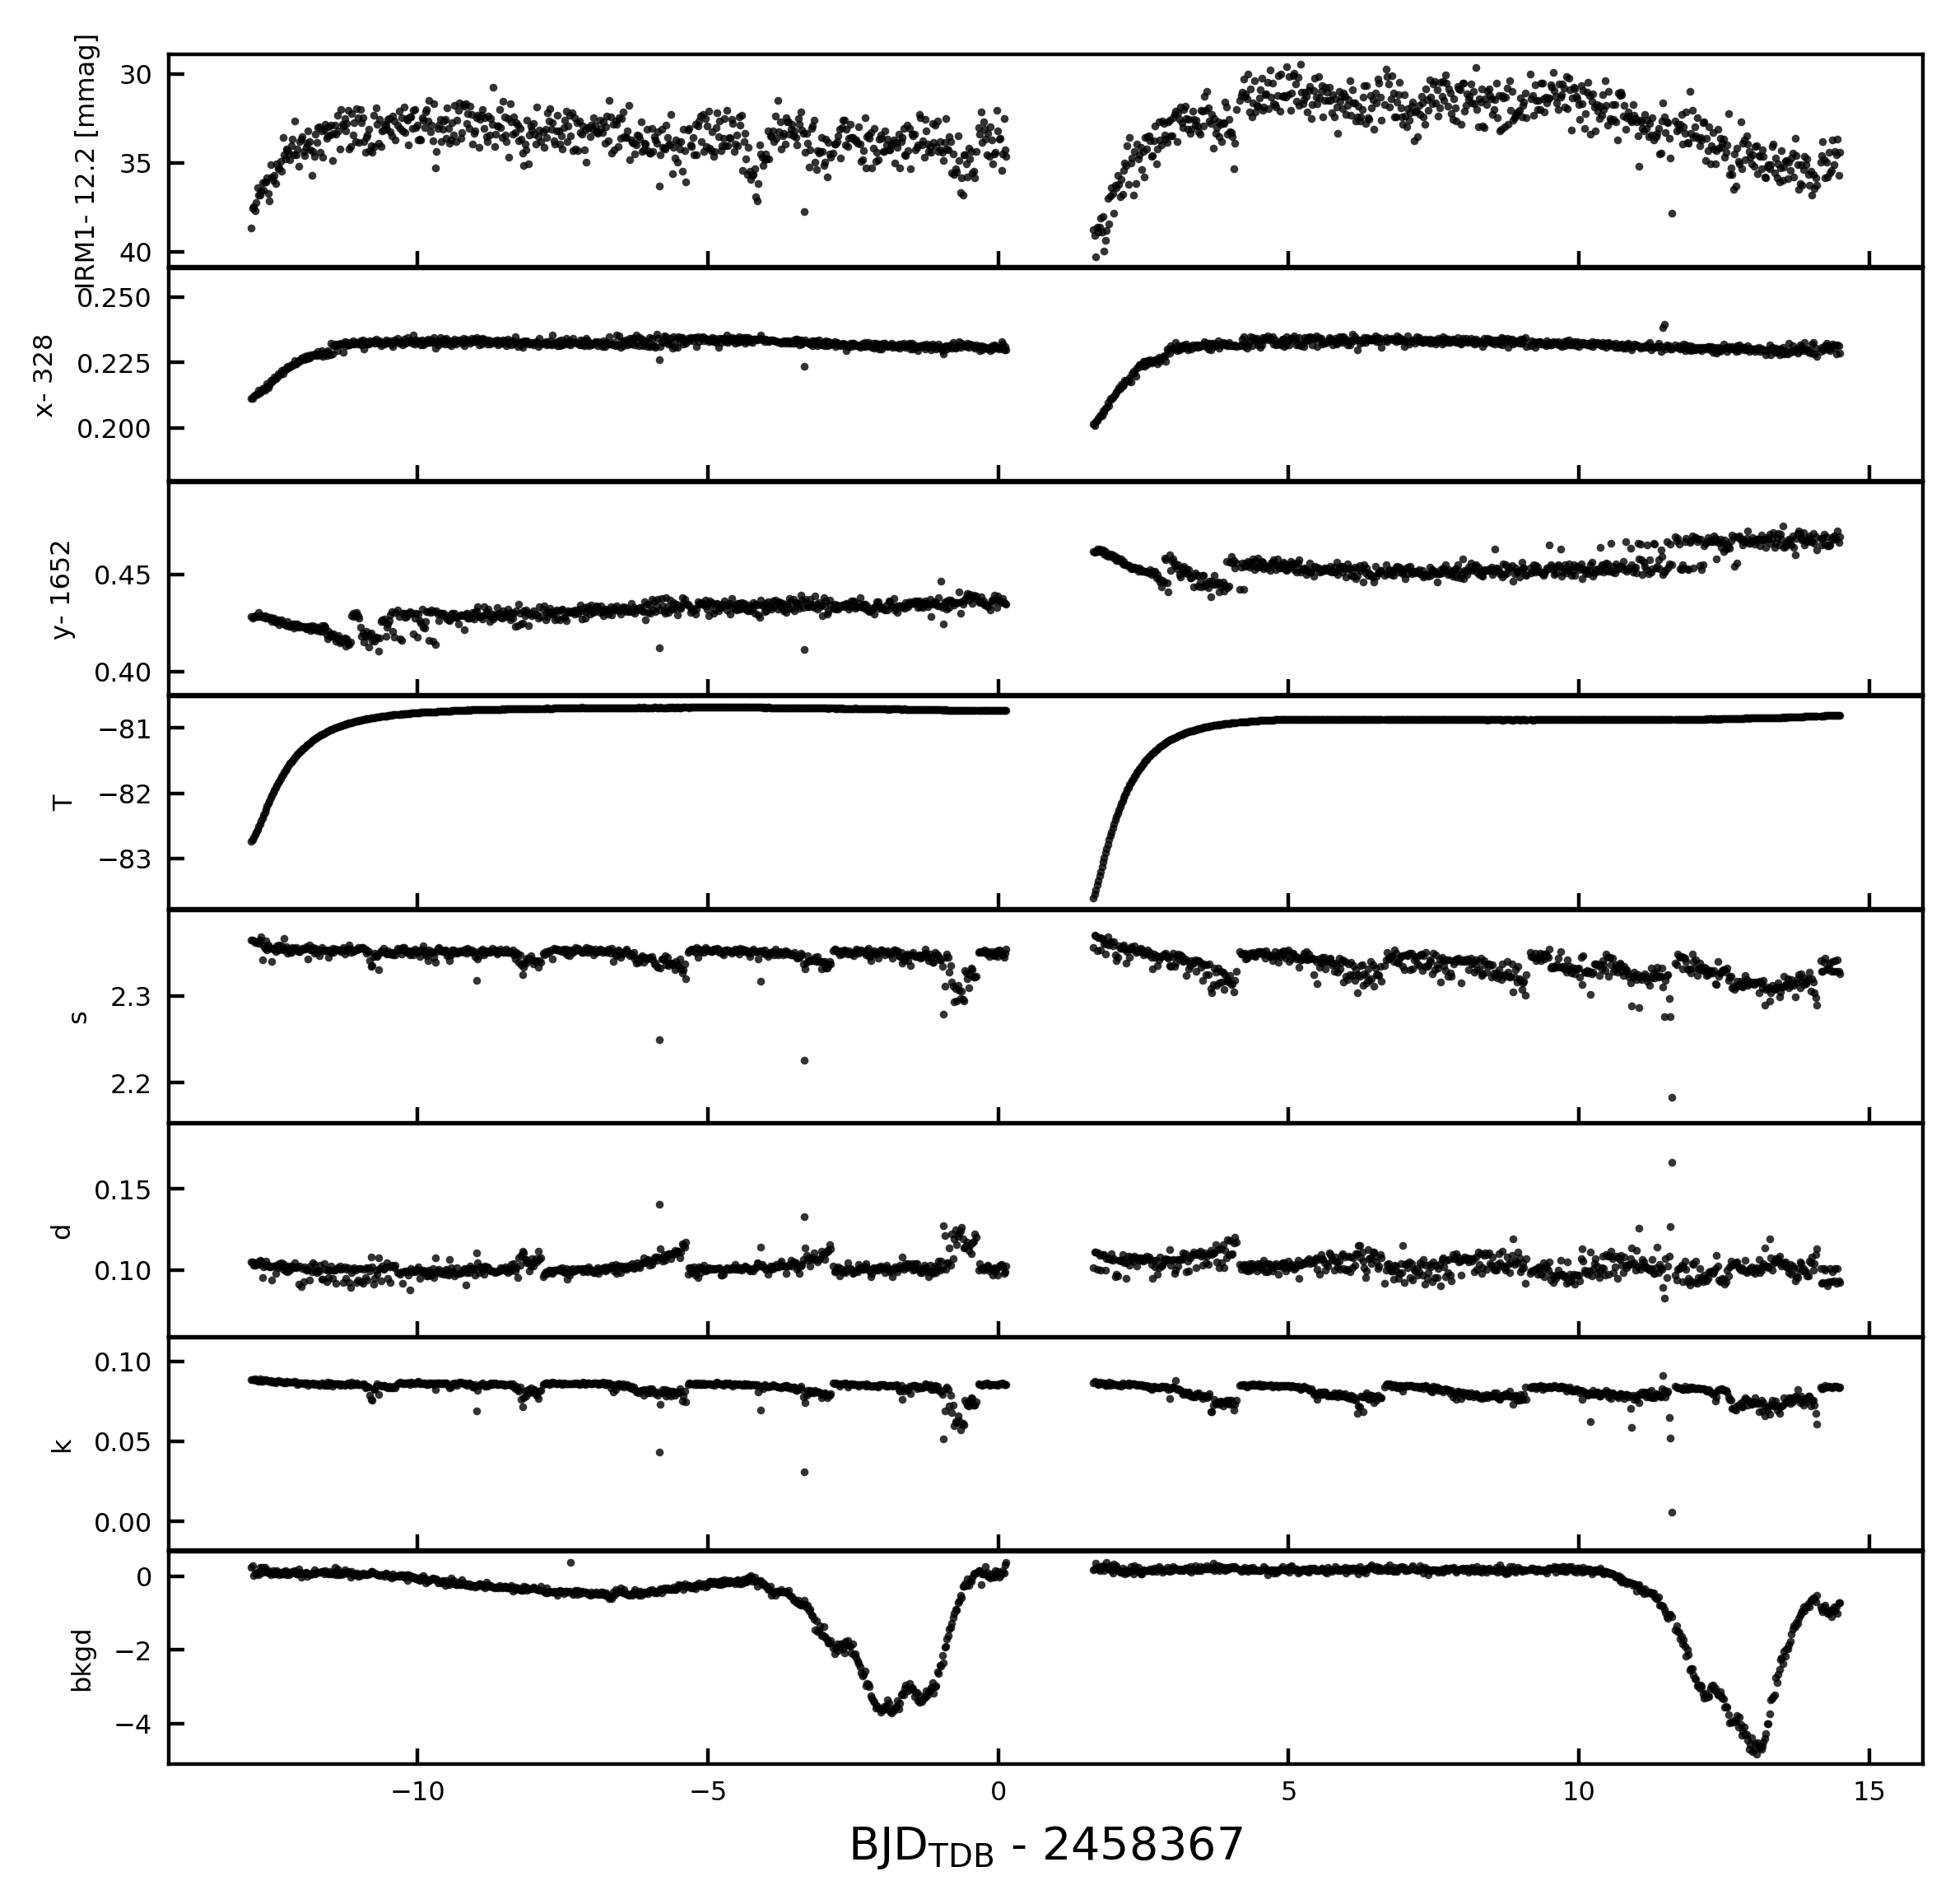
\includegraphics[width=0.47\textwidth]{epdparams_vs_time.png}
	\end{center}
	\vspace{-0.5cm}
	\caption{
		Timeseries of ``external parameters'' for a representative
			star over one sector.
			{\it Top}: Instrumental raw magnitude (with a particular
		aperture size), as a function of time.  {\it Second and third from
			top}: $x$ and $y$ centroid positions as a function of time.
		Continuing in order are the CCD temperature, the $(s,d,k)$ shape
		parameters, and the measured background value.
		Most of the apparent variability is instrumental.
		\label{fig:external_parameter_timeseries}
	}
\end{figure}
The preceding steps produce light curves that include both
instrumental systematics as well as astrophysical variability.  The
detrending approach adopted by the HAT group to remove systematic
variability typically proceeds in a few sequential stages, as
discussed by {\it e.g.} \citet{bakos_2010}, \citet{huang_high-precision_2015},
and \citet{zhang_precision_2016}.

The first detrending step commonly performed on ground-based data is
``magnitude-fitting'': the raw magnitudes measured from the difference
images are fit by a polynomial that depends on a combination of CCD
position, sub-pixel position, and optionally catalog magnitude and
color \citep[][\S~5.5]{zhang_precision_2016}.

The second step is to decorrelate against external parameters that are
known to affect the stellar flux measurements (EPD,
\citealt[][]{bakos_2010}).  For ground-based data this may
include zenith angle, or changing PSF parameters.  For TESS data, this
might include CCD temperature, or the angles of the Moon and Earth
relative to each camera's boresight.
Some example ``external'' parameters that we
include with our light curves are shown as functions of time in
Figure~\ref{fig:external_parameter_timeseries}.

The final step is to then decorrelate the measured brightnesses of
stars against each other (TFA, \citealt{kovacs_trend_2005}).  This
accounts for variations due to unknown systematic instrument changes
that affect many stars.  This latter step is similar to a principal
component analysis of all the light curves, in which the components
are chosen as a subset of the light curves.
In this sense TFA is similar to the Sys-Rem, PDC, and ARC2 methods
\citep{tamuz_correcting_2005,smith_pdc_2012,aigrain_robust_2017}
except that these latter methods make different choices for the basis
vectors, and apply different procedures for determining the
best-fitting coefficients of the linear model.

We explored the possibility of fitting linear models of flux as
functions of {\it e.g.,} temperature, shape parameters, centroid
positions, and stellar colors.  We also briefly explored non-linear
model fitting using $N$-dimensional B-splines to fit the flux,
centroid positions, and temperatures simultaneously
\citep{dierckx_curve_1996}.  The linear models typically underfit the
light curves, particularly during the large shifts that happen as the
spacecraft nears perigee.  The non-linear models showed some promise,
but often seemed to overfit stellar variability signals.  One thought
that we did not try but may explore in future work is to decorrelate
against the standard deviation of the spacecraft quartnerion time-series
\citep{vanderburg_hr858_2019}.

Given these complications, for the time being we omit the step of
``detrending'' as a function of external parameters. To enable further
exploration of the issue, we include all the necessary vectors of {\it
e.g.}, centroid positions, temperatures, and shape parameters in our
reported light curves.

% In \S~\ref{sec:flux_vs_external_parameters}, we describe the
% ``external parameter'' dependence visible in our reduction of
% the TESS data.
% Ordinary linear model-fitting, as well as an initial attempts
% at non-linear model fitting, are poor descriptions of the data.  
% In a similar vein ``magnitude-fitting'' is minimally justified, given
% how the TESS magnitudes correlate against these external parameters.
% We go on to show (\S~\ref{sec:tfa_is_good_enough}) that a plausible
% detrending approach for the purpose of transit discovery is to simply
% decorrelate against other nearby stars with standard TFA.
% 

% \subsubsection{Flux versus external parameters}
% \label{sec:flux_vs_external_parameters}
% 
% 
% % \begin{figure*}[t]
% %     \begin{center}
% % 		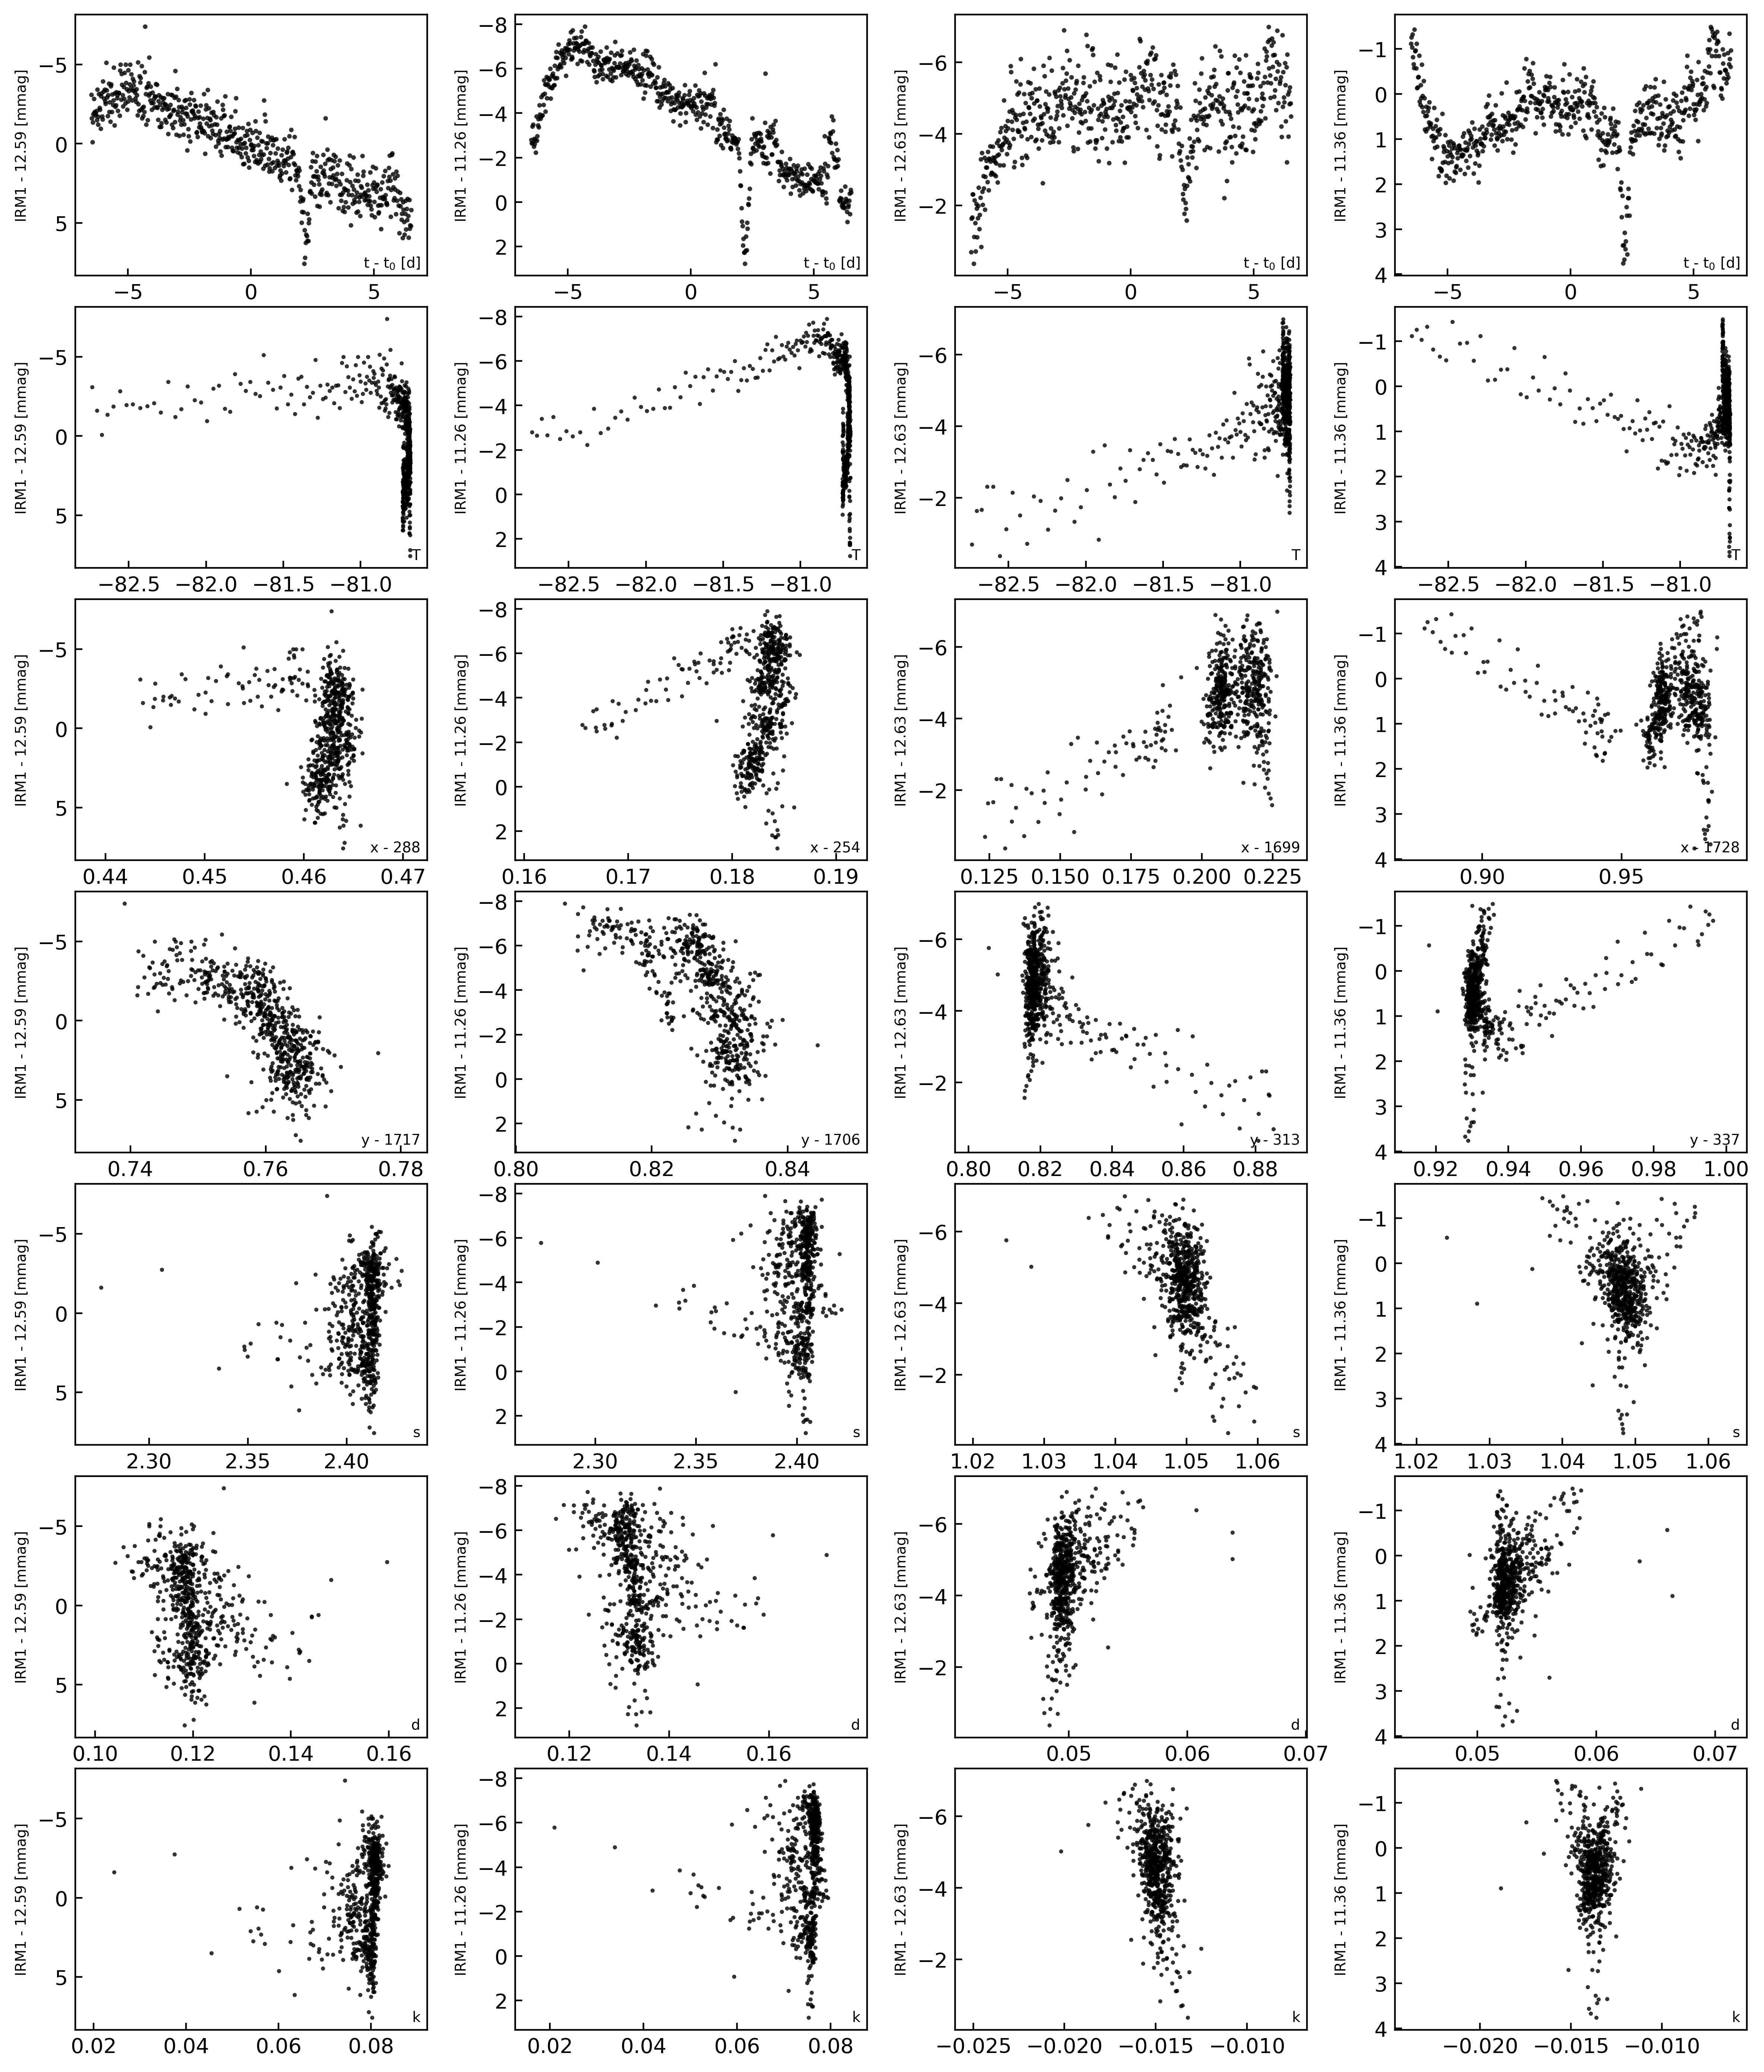
\includegraphics[height=0.9\textheight]{mag_vs_epdparams.png}
% %     \end{center}
% %     \vspace{-0.5cm}
% %     \caption{
% %       {\bf Flux as a function of ``external parameters'' for four
% %       representative stars.} The left two columns are stars at the
% %       corner of a camera's field; the right two columns are from the
% %       centers.
% %       Each row shows a different parameter along the $x$-axis, given
% %       in text at the bottom right of each subplot.
% %       ``Hooks'' are common features in flux as a function of
% %       temperature and centroid position.
% %       \S~\ref{sec:flux_vs_external_parameters} gives a verbose
% %       description.
% %      \label{fig:flux_vs_external_parameters}
% %     }
% % \end{figure*}
% 
% The traditional approach to EPD is to fit and
% subtract a model for the magnitudes $m$ of the form
% \begin{equation}
%   m = {\rm const.} + \sum_i c_i \theta_i,
%   \label{eq:classical_EPD}
% \end{equation}
% where $\vec{\theta}$ is a vector of parameters such as the shape
% parameters $(s,d,k)$, their products $(s^2, s\cdot d, d^2, \ldots)$,
% the temperature $T$ of the instrument or environment\footnote{ We used
% the temperature from the on-chip aluminum-copper sensor measurements
% included in the engineering
% data: \url{archive.stsci.edu/missions/tess/engineering/}.  },
% the centroid positions $(x,y)$, the fractional part of the
% centroid positions $(\{x\},\{y\})$, and any other parameters that are
% expected\footnote{ The fractional centroid positions might matter
% because intra-pixel quantum efficiency variations could affect the
% measured stellar brightness.  The varying temperature $T$ of the CCD
% electronics might matter.  } to correlate strongly with the observed
% flux.  The coefficients $c_i$ are calculated through linear
% least-squares, and subtracted to produce ``EPD'' light curves.
% 
% The premise of this model is that the correlations between the
% magnitudes and the external parameters are linear.  For ground-based
% CCD data (e.g., HATNet, HATS, and Nikon DSLRs), \citet{bakos_2010} and
% \citet{zhang_precision_2016} have verified that this model is a
% good description to the data.
% To discern whether such a model extends to the TESS data, we examined
% scatter plots of each parameter, as a function of all the other
% parameters.  We also examined plots of each parameter as a function of
% time.  A few prominent trends were present.
% 
% \begin{enumerate}
% 
% \item {\it Flux vs.\ time}. Most of the light curves we examined showed a secular
%     drift with amplitude $0.01\,{\rm mag}$ over the timescale of each
%     orbit.  Sharper trends (``hooks'') at the beginning of each orbit
%     seemed to be less prominent for stars at the corners of the fields
%     than stars at the center.  The periodicity incurred by the
%     2.5$\,{\rm day}$ momentum dumps was also noticeable in more of the
%     light curves at the center of the field than at the corners.
% 
% \item {\it Flux vs.\ centroid positions}. The flux as a function of
%   centroid position often showed non-linear ``hooks''
%     %(see Figure \ref{fig:flux_vs_external_parameters}).
%     Most of the data points from a given orbit reside at a given
%     level, but about 10\% are in a tail. This was seen in light curves
%     all across the TESS field of view.
% 
% \item {\it Flux vs.\ temperature} exhibited similar hooks, with most of
%   the flux values residing at a particular level, and perhaps 10\%
%     following a non-linear path (often resembling the Nike ``swoosh'')
%     away from the bulk of points.
% 
% \item {\it Flux vs.\ shape parameters}.  For light curves in the corner
%   of the field of view, similar hooks are present in flux {\it vs.}
%     $(s,d,k)$, though the hooks are less sharp.  In the center of the
%     field of view, gaussian ellipses are a better description of the
%     flux {\it vs.} the shape parameters.
%     
% \end{enumerate}
% 
% Considering the timeseries of parameters other than flux 
% (Figure~\ref{fig:external_parameter_timeseries}):
% 
% \begin{enumerate}
% 
% \item {\it Centroid positions vs\ time}.  The main variability in the
%   centroid positions as a function of time is a secular drift, that is
%     reset every orbit.  The 2.5 day momentum wheel dump is
%     superimposed on this secular drift, and has smaller amplitude than
%     the drift.
% 
% \item {\it Temperature vs.\ time}.  The main variability in temperature
%   {\it vs.} time is a secular drift of the same timescale as that for
%     the centroid positions timeseries.
% 
% \item {\it Shape parameters vs.\ time}.  The main variability in the
%   shape parameters as a function of time is the 2.5 day momentum wheel
%     dump periodicity, with hooks before each momentum dump.
% 
% \item {\it Background value vs.\ time}.  The background is typically stable, 
% except when scattered light from the Earth or Moon enters the frame (visible 
% towards the end of each orbit in 
% Figure~\ref{fig:external_parameter_timeseries}).
% 
% \end{enumerate}
% 
% Given the characteristics of the variability, a linear model of the
% form given in Equation~\ref{eq:classical_EPD} is not applicable.  To
% fit out the correlations between flux and parameters which most
% commonly exhibited ``hooks'', we explored fitting a parametric open
% curve (an $N$-dimensional B-spline, \citealt{dierckx_curve_1996}) to
% the flux, centroid positions, and temperatures simultaneously.  We
% selected the number of knots through brute-force, by calculating
% $\chi^2$ for the model fit over a grid of possible knots, and
% minimizing the Bayesian Information Criterion.  Though this approach
% showed some initial promise, even with ``optimal'' knot-selection (in
% the BIC sense) it introduced undesirable residuals in the light curves,
% and also distorted transits.
% One thought that we did not try but may explore in future work
% is to use the decorrelate against the scatter of the quartnerion 
% time-series \citep{vanderburg_hr858_2019}.
% 
% Given these complications, for the time being we omit the step of
% ``detrending'' as a function of external parameters. To
% enable further exploration of the issue, we include all the necessary
% vectors of {\it e.g.}, centroid positions, temperatures, and shape
% parameters in our reported light curves.
	

Since most of the external parameter dependence is shared between
stars, we opt instead to decorrelate the flux timeseries of each star
against other stars in the frame.  We use the TFA algorithm proposed
by \citet{kovacs_trend_2005}, which for self-consistency we describe
here.

The idea of the method is as follows.
Suppose we have $M$ ``template stars'', which are a subsample of
stars that represent all types of systematics across the dataset. 
Each template star has a light curve with $N$ data points.
Denote the template time-series $X_j(i)$, where $j={1,\ldots,M}$ and 
$i={1,\ldots,N}$ is the time index.
We then want to find periodic signals in a target time-series $Y(i)$.
This is done by defining a filter function
\begin{equation}
F(i) = \sum_{j=1}^{M} c_j X_j(i),
\end{equation}
for which the coefficients $c_j$ are found by minimizing
\begin{equation}
\mathcal{D} = \sum_{i=1}^{N} \left[ Y(i) - A(i) - F(i) \right]^2.
\label{eq:tfa_to_minimize}
\end{equation}
When trying to find periodic signals, $A(i)$ represents our prior
knowledge of the light curve's shape.
This prior is simply that stars on average maintain a constant brightness:
\begin{equation}
A(i) = \langle Y \rangle = \frac{1}{N} \sum_{i=1}^{N} Y(i) = {\rm const.}
\end{equation}
If a signal is eventually found, for instance using the box-least squares
method \citep{kovacs_box-fitting_2002},
this detrending process must then be repeated while accounting for our
updated knowledge about the light curve's shape.

Some implementation notes follow.
We selected template stars in two stages.
In the first stage, we fitted a parabola in the RMS-magnitude
plane, and discarded stars more than $2\sigma$ away from the
prediction of the fit.
We also required that these initial candidate stars have intermediate
brightness ($8.5 > T > 13$), and have a relatively large number
of time-series data points.
We then performed an initial iteration of TFA, on only the candidate
template stars.
We inspected the resulting detrended light curves for residual
structure by computing a Lomb-Scargle periodogram.
If the maximum-power peak had a false alarm probability below 0.1\%, 
we excluded the star from the list of candidate template stars, on the
basis of its presumed periodic variability.
We then randomly selected at most 200 template stars from the remaining
non-variable candidates. 
The choice of number of template stars was discussed by
\citet{kovacs_trend_2005}, and is another free parameter in
the broad problem of light curve production.
This choice is analogous to the issue of how many cotrending basis
vectors to choose in PDC-MAP or ARC2 \citep{aigrain_robust_2017}.
While the number of template stars can be optimized by constructing
and minimizing a BIC-like quantity, a little overfitting is acceptable
for our pupose of finding planetary transits.
For other applications, {\it e.g.,} stellar rotation period searches,
it is almost certainly preferable to adopt a less forceful
detrending approach.

Once the template stars were selected, we use the \texttt{VARTOOLS}
program to perform the detrending \citep{Hartman_Bakos_2016}.
This process was performed for each photometric aperture
separately.


%%%%%%%%%%%%%%%%%%%%%%%%%%%%%%%%%%%%%%%%%%
\section{Results}
\label{sec:results}

\begin{figure*}[!t]
	\begin{center}
		\leavevmode
		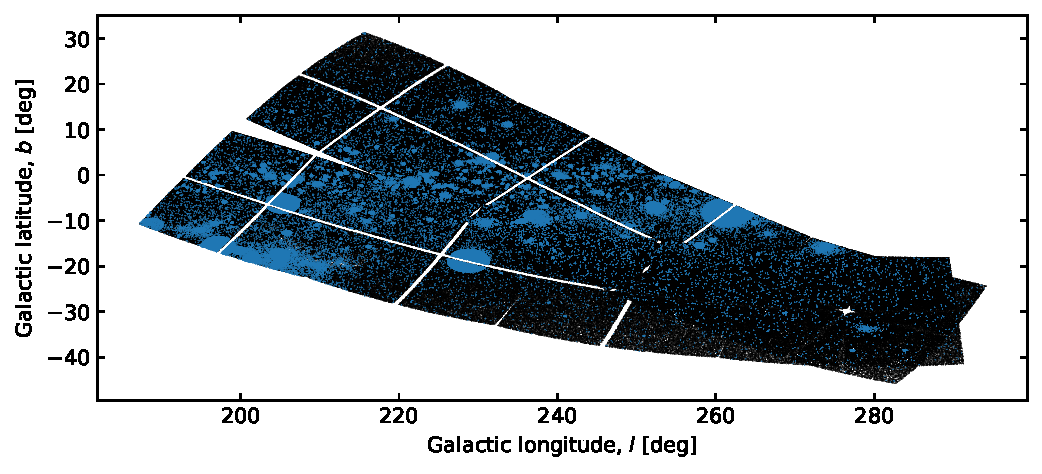
\includegraphics[width=0.9\textwidth]{galacticcoords_cluster_field_star_positions.pdf}
	\end{center}
	\vspace{-0.5cm}
	\caption{
		Positions of light curves from TESS Sectors 6
			and 7 in galactic coordinates.
		Black: $G_{\rm Rp}<13$ field stars.  Blue: $G_{\rm Rp}<16$
		target stars.  Target stars are mostly near the galactic
		plane. The data for Sectors 6 and 7 cover about one-sixth of
		the galactic plane.
		\label{fig:lcgalactic}
	}
\end{figure*}

%\begin{figure}[!t]
%	\begin{center}
%		\leavevmode
%		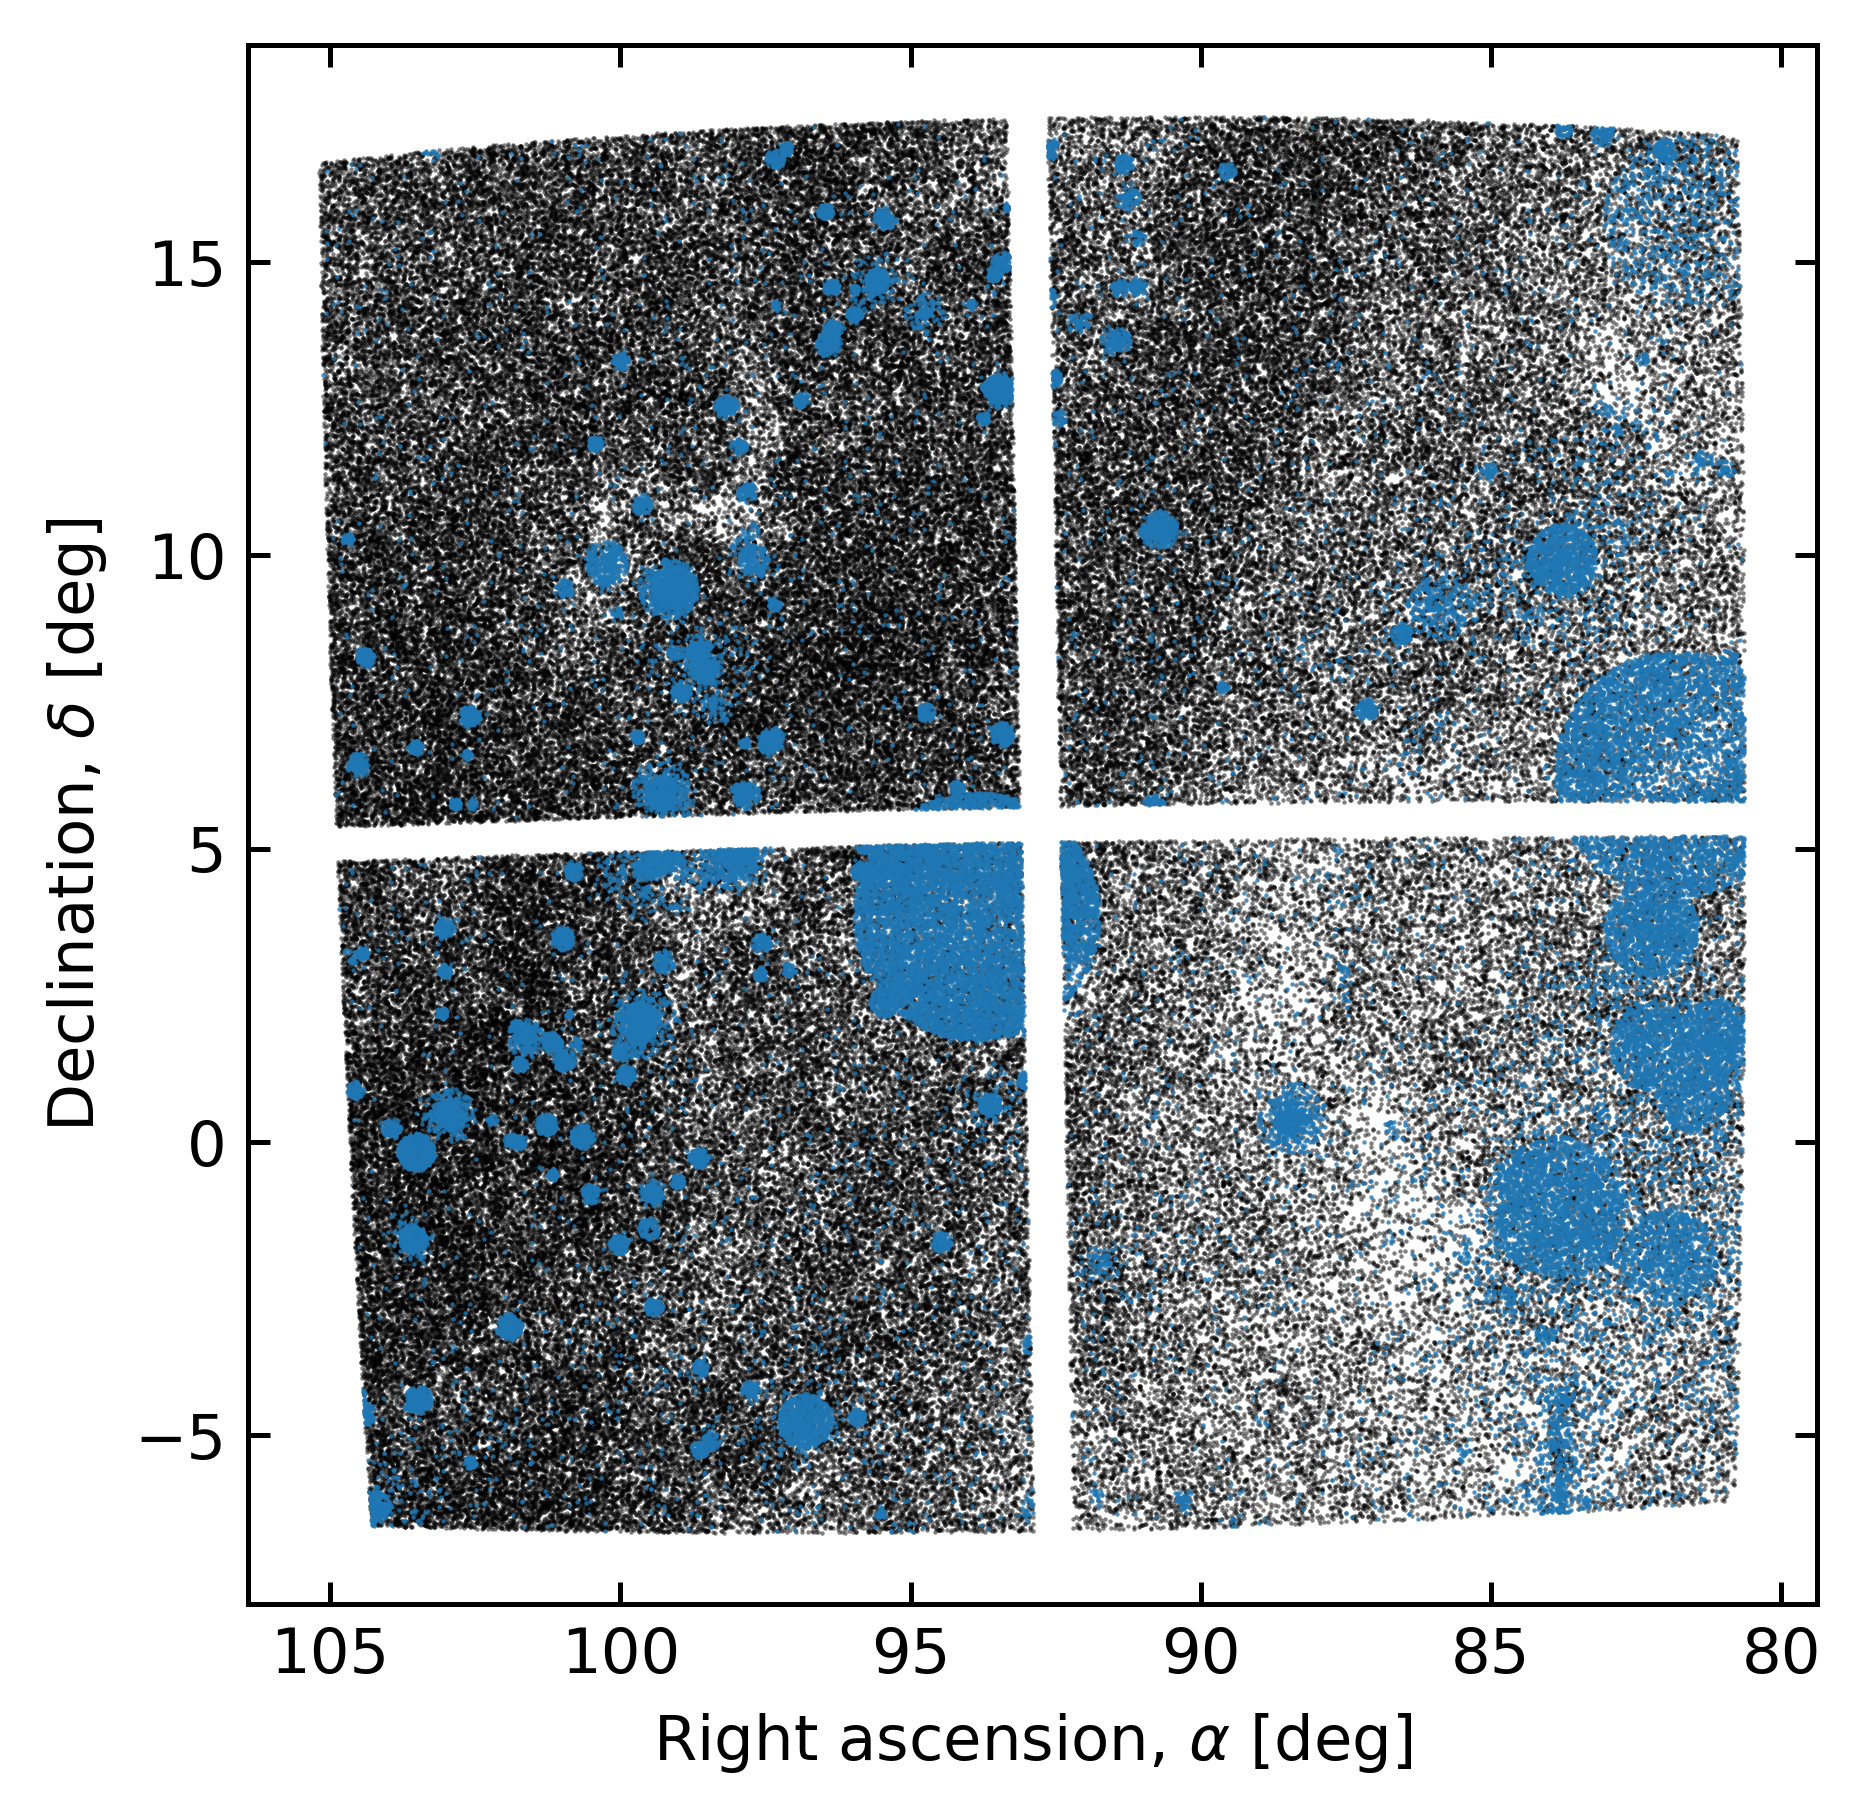
\includegraphics[width=0.47\textwidth]{sector6_cam[1]_ccd[1-2-3-4]cluster_field_star_positions.png}
%	\end{center}
%	\vspace{-0.5cm}
%	\caption{
%		{\bf  Zoom and coordinate transformation
%			of Sector 6, Camera 1 from Figure~\ref{fig:lcgalactic}.}
%		The most populated cluster is XXX, primarily due to candidate
%		members proposed by \citet{dias_proper_2014}.
%		\label{fig:lcradeczoom}
%	}
%\end{figure}


\begin{figure}[!t]
	\begin{center}
		\leavevmode
		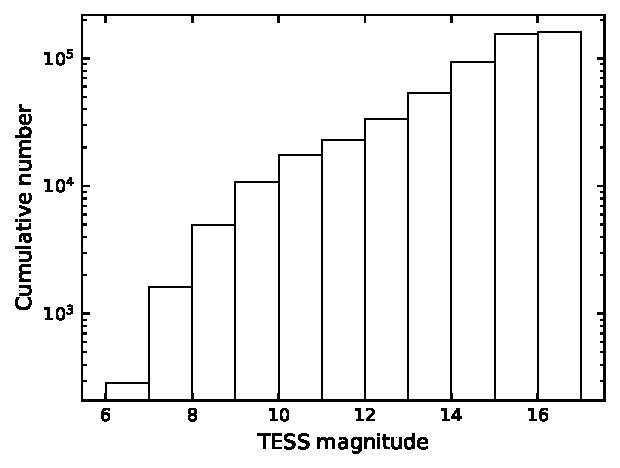
\includegraphics[width=0.45\textwidth]{cdf_T_mag.pdf}
	\end{center}
	\vspace{-0.5cm}
	\caption{
		Cumulative number of CDIPS light curves a function of TESS
			$T$-band magnitude.  Light curves were made for the
		target stars (Figure~\ref{fig:cdips_targets}) that were observed
		in Sectors 6 or 7.
		\label{fig:cdf_T_mag}
	}
\end{figure}

\begin{figure}[!ht]
	\gridline{\fig{hrd_scat_all_CDIPS_LCs.pdf}{0.45\textwidth}{}}
	\vspace{-0.8cm}
	\gridline{\fig{hrd_scat_close_subset.pdf}{0.45\textwidth}{}}
	\vspace{-0.8cm}
	\caption{
		{\it Top.} HR diagram of CDIPS stars on silicon in this
		data release.  {\it Bottom.} HR diagram of close CDIPS stars on
		silicon. The wedge separating the pre-MS sample from the MS
		stars was discussed by \citet{zari_3d_2018}, who introduced it in
		order to avoid contamination by photometric binaries.
	}
	\label{fig:hrd}
\end{figure}

\begin{figure}[!t]
	\gridline{\fig{pm_scat_all_CDIPS_LCs.pdf}{0.45\textwidth}{}}
	\vspace{-0.8cm}
	\gridline{\fig{pm_scat_close_subset.pdf}{0.45\textwidth}{}}
	\vspace{-0.8cm}
	\caption{
		{\it Top.} Proper motions of CDIPS stars on silicon in this
		data release.  Many of the stars in the central ``blob'' are possible
		field-contaminants.
		{\it Bottom.} Proper motions of close CDIPS stars
		on silicon.
	}
	\label{fig:propermotions}
\end{figure}

\begin{figure}[!t]
	\begin{center}
		\leavevmode
		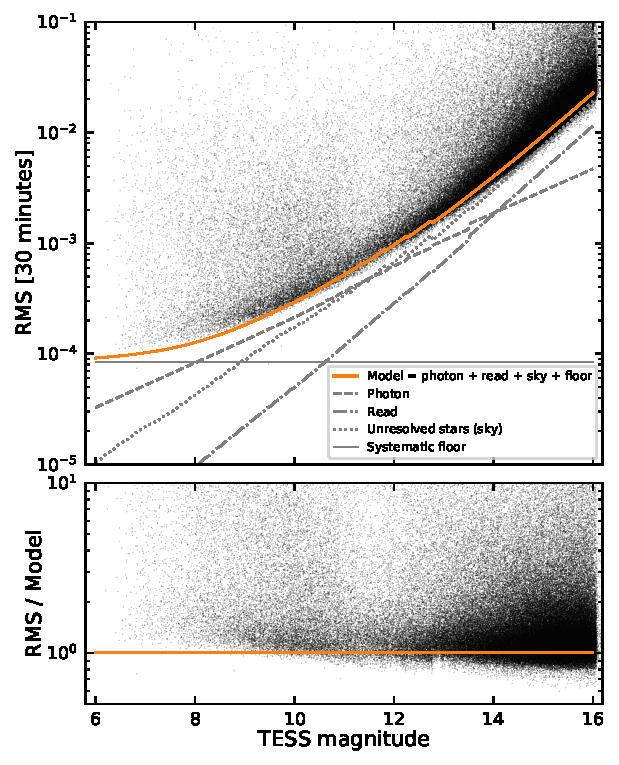
\includegraphics[width=0.47\textwidth]{rms_vs_mag.pdf}
	\end{center}
	\vspace{-0.5cm}
	\caption{
    Standard deviation of trend-filtered CDIPS light curves as a
    function of catalog TESS-band magnitude.  Black points correspond
    to the minimum RMS across the available three aperture sizes.  The
    model (orange and gray lines) assumes aperture sizes reported by
    \citet{Sullivan_et_al_2015}, and the effective area from
    \citet{vanderspek_2018}.  The noise from unresolved background
    stars (dotted gray line) is a function of galactic latitude, and
    dominates over zodiacal light for faint stars near the galactic
    plane; the line shown assumes a sight-line towards the center of
    Sector 6, Camera 1 (further details are in
    \S~\ref{subsubsec:rmsvsmag}).
		\label{fig:rms_vs_mag}
	}
\end{figure}

\begin{figure}[!t]
	\begin{center}
		\leavevmode
		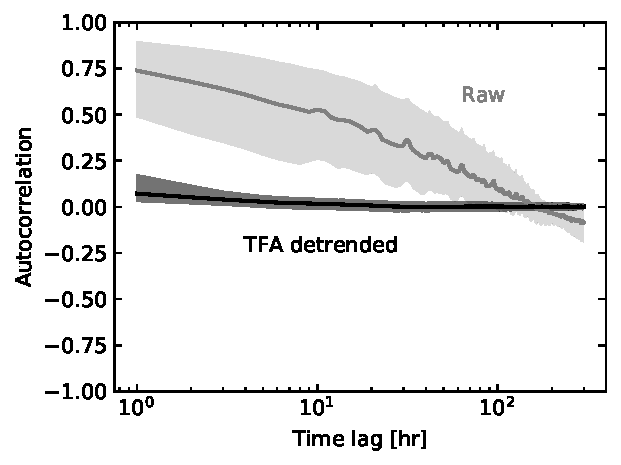
\includegraphics[width=0.47\textwidth]{avg_acf.pdf}
	\end{center}
	\vspace{-0.5cm}
  \caption{
    Average autocorrelations of $10^4$ randomly selected light curves
    from each sector.
    The medians at time lags spaced by one hour are shown for 
    raw light
    curves (column name \texttt{IRM}) in gray, and for
    TFA-detrended light curves in black.
    The gray bands display the 25$^{\rm th}$ to 75$^{\rm th}$ percentile
    range for each type of light curve.
  \label{fig:avg_acf}
	}
\end{figure}


\subsection{Light Curve Statistics}
\label{subsec:lcstatistics}

\subsubsection{Stellar properties}

The on-sky locations of the light curves from Sectors 6 and 7
are shown in Figure~\ref{fig:lcgalactic}.
Black stars are the field stars for which we performed photometry,
and of which a subset were used as template stars during TFA.
The blue stars are the \numberlcs stars with light curves available
from \stscilink.
Most of the target stars are quite close to the galactic plane.
Gaps between CCD chips are also visible.
The highly clumped nature of the target stars is also apparent.

%A zoom-in of Figure~\ref{fig:lcgalactic} is shown in Figure~\ref{fig:lcradeczoom}
%for the Camera 1, Sector 6 field. The effects of galactic-latitude
%dependent extinction are visible through the decreasing density of black
%points towards the right of the image.


Figure~\ref{fig:cdf_T_mag} shows the cumulative distribution of
TESS $T$-band magnitudes for the target stars.
Though most of the targets are faint, $\approx3\times10^4$ are
brighter than $T=13$. These targets are more promising for any
detailed follow-up observtions.

An HR diagram for the entire sample of CDIPS stars on silicon
is shown in Figure~\ref{fig:hrd} (top).
The sub-sample of stars with
measured positive parallaxes and naive distances less than
$1\,{\rm kpc}$ is also shown (bottom).
About one-third of the stars are in this latter sample.
The close stars are predominantly on the main-sequence, or the pre-main-sequence.
A relatively large fraction of these come from \citet{zari_3d_2018},
and are either on the PMS or upper main-sequence.
The latter set of OBA dwarf stars, while ``younger'' than the typical
field dwarf, are likely the least interesting subset of our target sample
from the perspective of age analyses.
In the entire sample (Figure~\ref{fig:hrd} top), a much larger fraction of stars are sub-giants,
red giants, and helium-burning red-clump stars.
We failed to obtain light curves for roughly $5\%$ of the stars on silicon, 
primarily due to our masking of saturated stars and their nearby pixels.

Finally, Figure~\ref{fig:propermotions} shows the proper motions of
the entire and close samples of stars on silicon.  Each clump
signifies a different star cluster. The largest overdensity in the top
figure is composed mainly of field star contaminants. It has two
subcomponents, due to the two different directions in the Galaxy being
observed in Sectors 6 and 7.



\subsubsection{Cluster membership provenance}

\paragraph{Sector 6}
In Sector 6, \sVInumberlcs light curves of candidate cluster stars
were made. The provenance of the claimed cluster origin of these
sources is \citet{dias_proper_2014} for 59\% of the sources;
\citet{zari_3d_2018} for 16\% of sources from their upper
main-sequence table and 1\% of sources from their PMS table;
\citet{Kharchenko_et_al_2013} for 8\% of sources,
\citet{cantat-gaudin_gaia_2018} for 6\% of sources, and more than two
catalogs for the remaining 10\% of sources.

The clusters with the largest claimed numbers of sources are the
Platais~6, Platais~5, and Mamajek~3 moving groups, all from
\citet{dias_proper_2014}, composing about 7000, 7000, and 3500 sources
respectively. These membership claims should be regarded with some
skepticism on a source-by-source basis.  For Platais~6,
\citet{Kharchenko_et_al_2013} claimed only about 400 probable members
(1$\sigma$) to exist within the angular radius of the cluster.
Mamajek~3 (= 32$\,$Ori) has only about 50 confirmed members
\citep{bell_32ori_2017}.

We remind the reader that our goal in creating our target catalog was
completeness, rather than fidelity. The \citet{dias_proper_2014} stars
in particular were included if they were listed with membership
probability exceeding 50\%.  To create cleaner sub-samples, we advise
use of the \texttt{CDEXTCAT} header keyword, which can be used
to merge against the original source catalog to obtain the
membership probabilities claimed by the original catalog.

\paragraph{Sector 7}
In Sector 7, \sVIInumberlcs light curves of candidate cluster stars
were made. The provenance of the claimed cluster origin of these
sources is  ... LGBTODO

The clusters with the largest claimed numbers of sources are ...
LGBTODO

\subsubsection{Light curve noise properties}
\label{subsubsec:rmsvsmag}

\paragraph{Observed RMS vs magnitude.}
The standard deviation of the TFA-detrended light curves is plotted as
a function of the catalog $T$-band magnitude for CDIPS light curves in
Figure~\ref{fig:rms_vs_mag}.
For the $y$-axis of this plot, we have taken
\begin{equation}
  {\rm RMS} = \left[
    \frac{1}{N-M-1}
    \sum_{i=1}^{N} (f_i - \bar{f})^2
  \right]^{1/2},
\end{equation}
where $f_i$ is the value of the flux at the $i^{\rm th}$ point in the
time-series, $\bar{f}$ is the mean flux, $N$ is the
number of points in the time-series, and $M$ is the number
of template light curves used during TFA detrending.
The correction in the denominator penalizes the natural degree of
overfitting inherent to the TFA algorithm.

The observed RMS (black points) follows the usual shape, with photon
noise dominating from $T=9$ to $T=12$, beyond which the onset of the
``sky'' background changes the overall slope of the curve to be more
steep.  For the brightest stars ($T\lesssim 9$), a ``systematic
floor'' was part of the mission's error budget
\citep{ricker_transiting_2015}, but has not been observed in early
reports of the photometric performance of various aperture photometry
pipelines ({\it e.g.,} the SPOC pipeline \citealt{jenkins_spoc_2010},
the MIT-QLP \citealt{huang_tess_2018}, and \texttt{eleanor}
\citealt{feinstein_eleanor_2019}).  The fact that our light curves for
the brightest stars are above this purported ``floor'', rather than
below it, suggests that our image subtraction techniques could be
introducing some small degree of noise to the light curves of the
brightest stars.  It is also true however that our largest aperture
contains only about 16 pixels, which is sub-optimal for stars brighter
than $T\approx9$ \citep[see][Figure~14]{Sullivan_et_al_2015}.  Since
the brightest stars are not the focus of the present work, we leave
this issue unaddressed for the time being.

Importantly, the faint stars do not noticeably exhibit
the typical effects of crowding at the faint end 
\citep[{\it e.g.},][Figure~5]{feinstein_eleanor_2019}.
In aperture photometry pipelines, stars in very crowded regions typically 
have their flux overestimated relative to the actual number of photons
that fall on silicon.
This leads to systematic underestimates of the uncertainty in the relative 
fluxes, as well as ``flux contamination'' (the reduction in amplitude of say, 
transit signals, due to diluting flux from neighbor stars).
Our method to work around this problem -- using the catalog magnitudes to 
predict the reference flux values, and measuring deviations from these 
reference fluxes on the subtracted images -- seems to be performing well.


\paragraph{Expected RMS vs magnitude.}

The noise model shown in Figure~\ref{fig:rms_vs_mag} is quite similar
to that of \citet{Sullivan_et_al_2015}, save for two changes.
The first change is that the effective area of the telescope is
updated to be $86.6\,{\rm cm}^2$, per the measurements by
\citet{vanderspek_2018}.

The second change is that we have explicitly included the
estimated noise contribution from unresolved faint stars.  The
brightness of the diffuse sky is dominated by different sources at
different wavelengths.  For instance, the CMB is most important in
the microwave, and thermal radiation from dust grains in the solar
system (zodiacal light) is dominant in the far infra-red
\citep{leinert_1997_1998}.  In the TESS-band, both zodiacal light and
faint stars can play a role, depending on the line of sight under
consideration. The zodiacal light is brightest near the ecliptic
plane, and the faint star background is brightest near the galactic
plane (and towards the galactic center).  
When performing pre-launch noise estimates,
\citet{winn_background_2013}
estimated the photon-counts from each component.
His zodiacal light model was presented by \citet{Sullivan_et_al_2015},
but the faint star component was not emphasized since the Sullivan
simulations were performed away from the galactic plane.

The diffuse sky model we have used for Figure~\ref{fig:rms_vs_mag} is
adopted explicitly because most of our target stars are near the
galactic plane.
Stars are judged to be ``unresolved'' and part of the background if
their surface density exceeds the angular resolution of the telescope.
TESS has an angular resolution of $\Delta \theta \sim 1'$, set by a
combination of the pixel size as well as the typical stellar FWHM.
Sources with sky surface density exceeding $\Delta \theta^{-2}$
therefore contribute to the background.

The relevant quantity needed to calculate the integrated 
photon counts from faint sources
is  $N(<m,l,b)$ --- the number of stars per square arcsecond
brighter than magnitude $m$, along a line of sight with galactic
longitude and latitude $(l,b)$.
To calculate this surface density, \citet{winn_background_2013}
queried the Besan\c con model
\citep{robin_synthetic_2003}  along a grid of galactic sight-lines,
and then converted to $I$-band surface brightnesses.
Fitting a smooth function to the results, \citet{winn_background_2013}
found
\begin{equation}
I\ {\rm mag\ arcsec}^{-2} =
    a_0 + a_1 \left(\frac{|b|}{40^\circ}\right)
    + a_2 \left(\frac{|l|}{180^\circ}\right)^{a_3},
\end{equation}
where the galactic longitude $l$ is measured from $-180^\circ$ to
$180^\circ$, and the empirical coefficients were found to be $a_0 =
18.9733$, $a_1=8.833$, $a_2=4.007$, and $a_3=0.805$.  This fit was
cautioned to be {\it very approximate}.  It is sensitive to the
threshold used to select ``unresolved'' stars, and likely no more
accurate than 0.5 mag on average.  In regions with exceptionally high
extinction ({\it e.g.}, star forming regions) it is expected to
systematic underestimate the background brightness by an even larger
degree.
Nonetheless, this model for the diffuse sky background seems
to agree reasonably well with the observed trend of standard deviation
versus stellar magnitude.


\paragraph{ACF statistics}

Beyond the white noise properties of the light curves, the red noise
properties are also important. 
In Figure~\ref{fig:avg_acf} we show the average autocorrelation of the
raw and TFA-filtered light curves.
The raw light curves have substantial systematic red noise; 
their average autocorrelation, evaluated at various time lags, is
positive.
The TFA-filtered light curves are much closer to gaussian~--~the
average autocorrelation between any two points in these light curves
is close to zero.
However, the average TFA-filtered light curve is not {\it exactly}
gaussian.
At time lags of a few hours or less, there is some excess power.
This suggests that additional detrending may be
necessary to maximize the effectiveness of planet searches (or the discovery of
any other signals via matched-filter techniques).


\subsection{Identifying Planet Candidates}
\label{subsec:identifying_ctois}

\begin{figure}[!t]
	\gridline{\fig{tls_sde_vs_period_scatter.pdf}{0.45\textwidth}{}}
	\vspace{-0.8cm}
	\caption{
    Transiting planet search periodogram summary.
    Each point represents the TLS periodogram peak signal detection
    efficiency (SDE) and corresponding period from one light curve.
    Significance thresholds (orange lines) are empirically defined for
    the transiting planet search described in
    \S~\ref{subsec:identifying_ctois}.  
    {\it Top.} Sector 6.  {\it Bottom.} Sector 7.
	}
	\label{fig:tlsresults}
\end{figure}


To identify an initial set of transiting planets, strong stellar
rotators, and eclipsing binaries, we performed a few steps of
post-processing on the light curves.  This processing was done
independently of the data release, since it was quite specific to our
own scientific interests.  The code used to do this additional
processing is also available
online\footnote{\url{github.com/lgbouma/cdips}, commit
\texttt{348eea7}.}.

For simplicity, we first chose a single aperture size~--~``aperture
2''~--~with a radius of 1.5  pixels.  Then, to identify periodic
transit-like signals, we used \citet{hippke_TLS_2019}'s transit
least-squares (TLS) tool.  The algorithm is the same as the canonical
box least-squares \citep{kovacs_box-fitting_2002}, except in place of
a box template, a transit template is used  for a marginal improvement
of the detection efficiency.  In addition, the search grids in
\texttt{tls} \footnote{\url{https://github.com/hippke/tls}} are
slightly more efficient than in most BLS implementations, since
\texttt{tls} uses the cubic-in-frequency sampling advocated by
\citet{ofir_optimizing_2014}, rather than standard linear-in-frequency
sampling.  Our grids typically consisted of about 30 different
durations, and about 5000 periods between 0.5 and 21 days. 

Before performing the period search, we rejected $6\,{\rm hours}$ at
the beginning and end of each spacecraft orbit, to mitigate the
presence of correlated red noise in the results.  This shrank the data
volume by about 5\%, but also lowered the number of systematic false
positives in subsequent vetting.  We then performed an asymmetric
sigma-clipping of $(50\sigma,5\sigma)$ about the median to preserve
transits while omitting flares and other positive flux excursions. 

A number of the light curves show residual variability, often of
stellar origin.  This is expected for a sample of young stars; the
problem of finding transits in the face of large stellar rotation
signals has been explored by both \citet{rizzuto_zeitV_2017} and also
\citet{hippke_wotan_2019}.  The former adopted an approach that we
have yet to explore, which is to pass a sliding window over the light
curve that, within each step, performs a Bayesian model comparison
between a spline and a spline-plus-notch model.  If the
spline-plus-notch model is favored, the transits are preserved for
subsequent discovery.  \citet{hippke_wotan_2019}, conversely,
described a number of different detrending methods, and found that
most performed more or less the same at recovering planetary transits
for a sample of young stars with strong rotation signals.

Our approach in this work is essentially identical to one of the
methods described by \citet{hippke_wotan_2019}.  First, before
sigma-clipping or omitting points near the edges of orbits we run a
generalized Lomb-Scargle periodogram on each TFA light curve
\citep{lomb_1976,scargle_studies_1982,vanderplas_periodograms_2015}.
If a peak is found with false alarm probability below $10^{-5}$, we
consider the star ``variable'', and opt to detrend the flux timeseries
with robust penalized B-splines, which are splines with knot-length
automatically determined via cross-validation
\citep{eilers_flexible_1996}. The idea behind the cross-validation is
that more knots leads to smaller residuals on training data, but
larger errors when tested on the entire dataset.  We used the
\texttt{wotan} implementation, which is a wrapper to the
\texttt{pyGAM} spline fitter, with $2\sigma$ clipping of outliers from
the fit residuals at each iteration
\citep{serven_pygam_2018_1476122,hippke_wotan_2019}.  The maximum
number of spline knots is set to 50, which for each TESS sector
($\approx 25\,{\rm days}$) is commensurate with a $\approx0.5\,{\rm
day}$ window.

We verified by injecting and recovering a 2.5 mmag, zero impact
parameter 
planet with variable period that this detrending approach marginally
improved the recovery probability, compared to not doing anything.
The main cases for which it helps are those with large residual
stellar variability in the TFA light curve.

After (optionally) detrending, we run the TLS search. To select
``significant'' signals for visual inspection, we performed a cut on
the TLS signal detection efficiency defined piecewise over the signal
periods.  The overall lower limit is ${\rm SDE} > 12$, with higher
limits imposed in regions with heavy contamination from systematic
signals.  The signals for sectors 6 and 7 are shown in the space of
SDE vs period in Figure~\ref{fig:tlsresults}.

This yielded a few thousand light curves.  About two-thirds already
had been detrended with splines, and were not processed further.  For
the remaining third we performed TFA signal reconstruction using
\texttt{VARTOOLS}.  In this process, the model lightcurve $A(i)$ in
Equation~\ref{eq:tfa_to_minimize} is set to the phase-binned signal
from the most powerful peak in the TLS spectrum, rather than being a
constant function.  This helps lower the scatter of the light curve at
frequencies away from the TLS peak.

We then make a multi-page \texttt{.pdf}-format document report with
the information necessary to make classifications for vetting.  These
vetting reports are released along with the light curves, and are a
useful summary for anyone interested in the subset of objects that we
have analyzed.  A full description of each page of the report is given
in Appendix~\ref{appendix:vetreport}.
When classifying these reports, we assessed:
\begin{enumerate}
    \item {\it Morphology of photometric variability}. Designations
      include tags for planet candidates, eclipsing binaries,
      instrumental variations, stellar variations, and ``weirdos''.
    %
    \item {\it Cluster membership status}. By default, all light
      curves were made for stars with at least one literature claim of
      cluster membership.  However, some of these claims pre-dated the
      availability of Gaia-DR2 parallaxes or proper motions.  We
      therefore re-assess the membership status on a case-by-case
      basis through inspection of the available astrometry and
      photometry.  Known asterisms are also omitted at this point
      \citep[{\it
      e.g.},][]{sulentic_revised_1973,baumgardt_asterisms_1998,kos_galah_2018}.
    %
    \item {\it Photometric blends}. Tags are created to highlight
      whether the depth of the photometric signal shows a strong
      dependence on aperture size, and also whether the in-transit
      minus the out-of-transit images reveal that the source of
      variability is in fact far from the target star.
\end{enumerate}
The initial classifications were performed by LGB, and possible
planet candidates were then vetted by JH and JNW.
The \texttt{TagSpaces}
software was used to easily assign labels to the documents.


\subsection{Candidate TESS Objects of Interest}
\label{subsec:ctois}

\begin{figure*}[!t]
	\begin{center}
		\leavevmode
		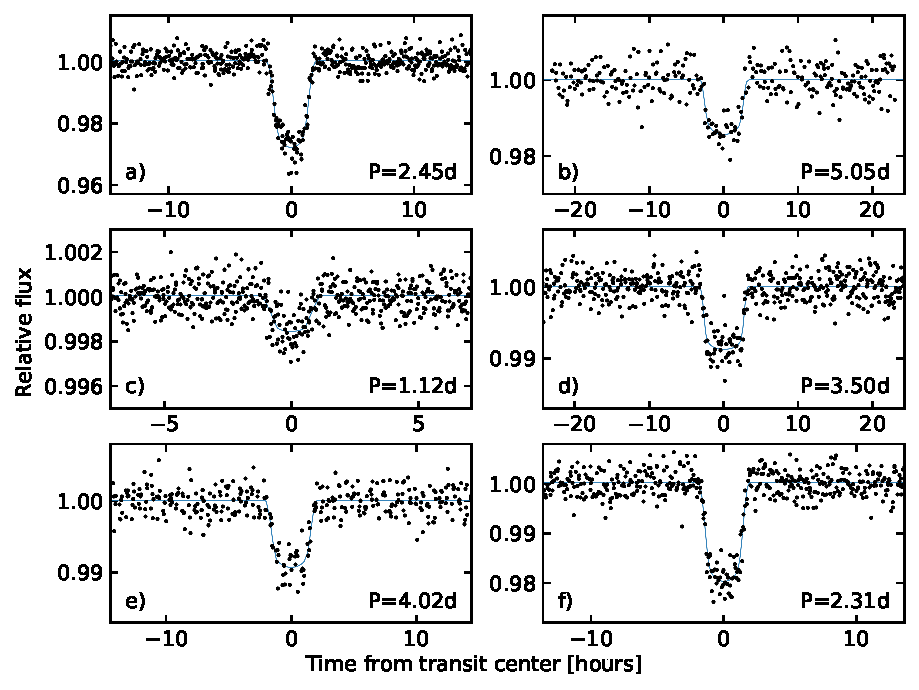
\includegraphics[width=0.9\textwidth]{quilt_PCs.pdf}
	\end{center}
	\vspace{-0.2cm}
	\caption{
		Phased light curves for six of the \numberpcs candidate
			transiting planets identified in this work.
		Black points are detrended flux measurements, phased to the
		best-fit orbital period indicated in the lower right of each
		panel.
    Transit models are fitted as described in \S~\ref{subsec:ctois},
    and plotted with blue lines.
		For display purposes, a window of $\pm 4$ transit durations
		centered on the transit mid-point is displayed.
		The vetting reports for these objects are available at XXX.	%FIXME
		% TODO: include age? T mag?
		The Gaia source identifiers are
		a): 5605128927705695232, 
		b): 3125263468681400320, 
		c): 5510676828723793920, 
		d): 3007171311355035136, 
		e): 5617126180115568256, 
		f): 3220266049321724416.   
		\label{fig:ctoi_quilt}
	}
\end{figure*}

\begin{figure}[!t]
	\begin{center}
		\leavevmode
		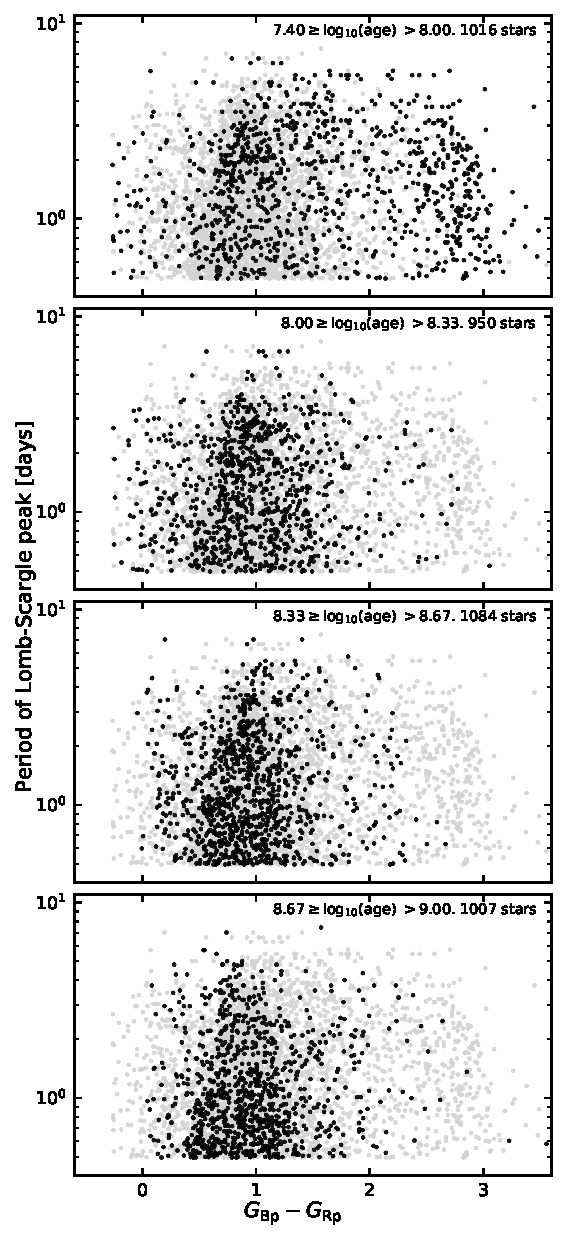
\includegraphics[width=0.45\textwidth]{LS_period_vs_color_and_age.pdf}
	\end{center}
	\vspace{-0.2cm}
	\caption{
    Time evolution of Lomb-Scargle periodogram peak period versus Gaia
    color.
		Red stars are on the right, blue stars are on the left.
		Each point on this diagram is a star for which the false alarm
		probability of the most powerful Lomb-Scargle peak is below
		$10^{-15}$.
		Additionally, we required (1) that the membership claim originate
		from \citet{cantat-gaudin_gaia_2018},
		\citet{Kharchenko_et_al_2013}, or \citet{gaia_hr_2018}; and (2)
		that the cluster with claimed membership had an age reported by
		\citet{Kharchenko_et_al_2013}.
		Our approach for avoiding photometric blends is described in
		\S~\ref{subsec:notplanets}.
		\label{fig:ls_peak_vs_time}
	}
\end{figure}


If all vetters identified an object as a planet candidate, we then
proceeded to fit a transit model to the data.  The procedure closely
mirrors that used by \citet{bouma_wasp-4b_2019} to create a
phase-folded light curve for WASP-4.

First, we selected points within 5 transit durations of each transit
midpoint, using the orbital period, transit duration, and reference
epoch found from applying TLS to the detrended light curve.  We then
fitted a line to the out-of-transit flux measurements around each
transit window, and divided it out.  We then fitted a standard transit
model using the formulae given by \citet{mandel_analytic_2002} and
implemented by \citet[][\texttt{BATMAN}]{kreidberg_batman_2015}.  The
free parameters were the orbital period, the reference epoch, the
planet to star radius ratio $R_{\rm p}/R_\star$, the orbital distance
to stellar radius ratio $a/R_\star$, and the inclination $i$.  We
assumed circular orbits.  To fix the quadratic limb-darkening
parameters, we collected $T_{\rm eff}$ and $\log g$ from the TIC, and
then interpolated against the \citet{claret_limb_2017} tables.  For
stars hotter than the maximal effective temperature of these tables
($12,000\,{\rm K}$), we simply used the coefficients of the hottest
star.

We then sampled the posterior probability distribution using the
\citet{goodman_ensemble_2010} algorithm, as implemented by
\citet[][\texttt{emcee}]{foreman-mackey_emcee_2013}.  Our main goal in
this procedure was to provide an accurate ephemeris.  To ensure that
the reported uncertainties are valid, after performing the initial fit
using the photometric uncertainties reported in our light curves, we
rescaled the the uncertainty in each photometric data point to equal
the root-mean-square deviation of each transit-model subtracted light
curve. We then refitted each light curve.

The resulting parameters are given in Table YYY, and are also
available as cTOIs NNN.01 - MMM.01 on exofop-TESS (LINK).
Figure~\ref{fig:ctoi_quilt} shows the phase-folded lightcurves and
their best-fitting moels.

The physical parameters quoted in Table YYY, and on exofop-TESS,
should be considered preliminary, and could be substantially improved
with an object-by-object analysis.  A few additional assumptions were
required to report some of the values.  For the stellar radii, we
assumed the $R_\star$ values and uncertainties reported in the TIC.
There were a few cases with null uncertainties in the stellar radii --
for these, we simply invented a relative uncertainty of 30\%, and note
in the comments that this was done.  There were also a few cases for
which the TIC stellar temperatures and/or radii were not available,
but the Gaia values were.  In these cases, we used the Gaia $T_{\rm
eff}$ and $R_\star$ values \citep{andrae_apsis_2018}, and a stellar
mass interpolated from the \citet{pecaut_intrinsic_2013} table
(assuming the star is a dwarf) to estimate $\log g$ for the
limb-darkening.  The uncertainties in e.g., the planetary radii and
impact parameters were found using linear error propagation theory,
under the idealized assumption that the covariance between all stellar
and planetary parameters was zero.

Finally, to assign the names of the planet candidates -- and determine
whether they had already been identified as TOIs or cTOIs -- we used
lists downloaded from the \url{tev.mit.edu} alert site for TOIs, and
from \url{exofop.ipac.caltech.edu/tess} for cTOIs.  We
cross-referenced based on a combination of the TIC identifier, spatial
position, and the ephemeris of each object.


\subsection{Eclipsing binaries, stellar rotation}
\label{subsec:notplanets}

To assess the prospects for studying forms of stellar variability
other than that caused by transiting planets, we performed a brief
additional exploration.
Using the Lomb-Scargle periodogram results from
\S~\ref{subsec:identifying_ctois}, we selected light curves 
for which the periodogram peak power had a corresponding false alarm
probability below $10^{-15}$.
We chose this cutoff to be small enough to give us a reasonable number
of objects, but large enough so that there would be no question that
the signal being detected was astrophysical.

Further, we then restricted our focus to stars with a cluster
membership claim in \citet{cantat-gaudin_gaia_2018},
\citet{Kharchenko_et_al_2013}, or \citet{gaia_hr_2018}, since from our
experience these works have a relatively low false positive
probability.
We then further restricted our sample of stars to be those for which
the claimed cluster also had an age reported by
\citet{Kharchenko_et_al_2013}.

To remove obvious photometrically-blended duplicates, for any signal,
if any nearby stars had matching periods, we kept only the signal with
the lowest false alarm probabilty.
While this does not ensure that the detected signals originate from
the target star, it removed a large number of the duplicate signals,
and suits our exploratory purposes.

All told, this yielded 4057 stars between the ages of about 25 Myr and
1 Gyr.
In Figure~\ref{fig:ls_peak_vs_time}, we plot the Lomb-Scargle peak period
versus $G_{\rm Bp} - G_{\rm Rp}$ color over four different bins of
time.
The bins were chosen to match the sub-sample sizes within reasonable
proximity.

The youngest sample of stars is the reddest, as might be expected
given that many of these stars have not yet reached the main sequence,
and may exist along lines of sight with heavy extinction.
Stars younger than about 200 Myr (the first two age bins) also tend
to be bluer.
The oldest stars, between about 450 Myr and 1 Gyr, show a hint in
the detected periods of being ``bottom-heavy'', {\it i.e.}, there are
relatively more short-period objects in this sample.
The reason why is unclear~--~the effect could be due to systematic
differences in the stellar samples, rather than being astrophysical.
More investigation will be required.



%%%%%%%%%%%%%%%%%%%%%%%%%%%%%%%%%%%%%%%%%%
\section{Discussion}
\label{sec:discussion}

Maybe JH or JNW could work on these subsections?

\subsection{The planet candidates require more observations}
Additional observations are needed for two major goals:
a) cluster membership confirmation
(age indicators, across the board);
b) verify the planetary nature of the signals
(seeing-limited photometry, RV mass measurement).

Different types of observations and analyses are needed to confirm 
(i) the planetary nature of these signals, and
(ii) whether the host stars are bonafide cluster members.
For (i), follow-up photometry, high-resolution imaging, and in some
cases spectroscopic mass measurement are needed.
For (ii), one or two radial velocity measurements might kinematically
exclude cluster membership in a number of cases.
A full assessment of the target star's age indiciators, including
photometric rotation signatures, spectroscopic Li and H$\alpha$
measurements, and even an isochronal analysis, would be helpful.

\subsection{Eclipsing binary and stellar variability analyses may also
be feasible}

JH?


%%%%%%%%%%%%%%%%%%%%%%%%%%%%%%%%%%%%%%%%%%
\section{Conclusion}
\label{sec:conclusion}

%FIXME: paraphrase / improve all the below
In this study, we first collected an all-sky sample of about one million
candidate young stars brighter than $G_{\rm Rp}$ of 16.
82\% of the target star sample resides in a ``cluster'', a generic
term we adopted for open clusters, stellar associations, and moving
groups.
The remaining stars have photometric or astrometric indications of
their youth, and either reside on the pre-main-sequence or upper
main sequence.

We then reduced TESS full frame images taken over the course of about
two months (Sectors 6 and 7; the first fields very close to the galactic
plane).
We performed difference imaging in order to minimize the complications
of the crowded background.
Using forced aperture photometry, we made light curves for all stars
brighter than $G_{\rm Rp}$ of 13, and went three magnitudes deeper for
our target star sample.
This yielded \numberlcs light curves of candidate young stars across
\numberclusters distinct clusters.

The light curves seem to be limited in precision by photon noise at
the bright end, and by unresolved background stars at the faint end.
Though the raw light curves show significant red noise, decorrelating
against a set of template stars led to an ensemble of light curves
with very nearly gaussian noise properties.

An initial search for transiting planets, along with subsequent
vetting to remove obvious non-cluster members and photometric blends,
has revealed \numberpcs planet candidates.
\numberclusterpcs of these candidates are candidate cluster members,
and the remaining \numberzaripcs have indications of youth, relative
to field stars.
The latter sub-sample is the less interesting one for this work, but
may be of interest for other studies.
Substantial follow-up efforts on these objects are needed to determine
(i) whether the candidates are planets and (ii) whether the host stars
are truly cluster members.
We suspect that a sizeable fraction of our planet candidates may
be eclipsing binaries, however it likely also includes real planets.
The vetting reports are available at \stscivetlink, and also documented
in Appendix~\ref{appendix:vetreport}.
The planet candidate parameters are on exoFOP-TESS.

We also briefly explored other forms of photometric variability in the
dataset.
The age-evolution of extremely high-SNR variability seems to show some
evolution in the space of LS peak-period versus color
(Figure~\ref{fig:ls_peak_vs_time}), but interpreting this result will
require a more careful exploration.
In searching for transiting planets, we found many eclipsing binaries,
as well as stellar rotation and pulsation signals.
Those who wish to explore the time-evolution in these and any other
systems are invited to explore the data at \stscilink.





\acknowledgements
L.G.B.\ gladly acknowledges helpful discussions with
C Huang, M Soares-Furtado, ...
..., and is
grateful to the people who have turned TESS from an idea into reality.
%
J.N.W.\ thanks ...
%
This paper includes data collected by the TESS mission, which are
publicly available from the Mikulski Archive for Space Telescopes
(MAST).
%
Funding for the TESS mission is provided by NASA's Science Mission
directorate.
%
This research has made use of the NASA Exoplanet Archive, which is
operated by the California Institute of Technology, under contract
with the National Aeronautics and Space Administration under the
Exoplanet Exploration Program.
%
This work made use of NASA's Astrophysics Data System Bibliographic
Services.
%
This research has made use of the VizieR catalogue access tool, CDS,
Strasbourg, France. The original description of the VizieR service was
published in A\&AS 143, 23.
%
This work has made use of data from the European Space Agency (ESA)
mission {\it Gaia} (\url{https://www.cosmos.esa.int/gaia}), processed
by the {\it Gaia} Data Processing and Analysis Consortium (DPAC,
\url{https://www.cosmos.esa.int/web/gaia/dpac/consortium}). Funding
for the DPAC has been provided by national institutions, in particular
the institutions participating in the {\it Gaia} Multilateral
Agreement.
%
The Digitized Sky Surveys were produced at the Space Telescope Science Institute under U.S. Government grant NAG W-2166. The images of these surveys are based on photographic data obtained using the Oschin Schmidt Telescope on Palomar Mountain and the UK Schmidt Telescope. The plates were processed into the present compressed digital form with the permission of these institutions.
%
\newline
%
\facility{
	2MASS \citep{skrutskie_tmass_2006},
	Gaia \citep{gaia_collaboration_gaia_2016,gaia_collaboration_gaia_2018},
	TESS \citep{ricker_transiting_2015},
	UCAC4 \citep{zacharias_fourth_2013}
    %DSS (CITE)    
}
%
\software{
  \texttt{astrobase} \citep{bhatti_astrobase_2018},
  \texttt{astropy} \citep{the_astropy_collaboration_astropy_2018},
  \texttt{astroquery} \citep{astroquery_2018},
  %\texttt{astroquery.gaia} CITE,
  %\texttt{astroquery.simbad} CITE,
  %\texttt{astroquery.mast} CITE,
  %\texttt{astroquery.nasaexopanetarchive} CITE,
  \texttt{BATMAN} \citep{kreidberg_batman_2015},
  \texttt{corner} \citep{corner_2016},
  \texttt{emcee} \citep{foreman-mackey_emcee_2013},
  \texttt{fitsh} \citep{Pal_2012},
  \texttt{IPython} \citep{perez_2007},
  \texttt{matplotlib} \citep{hunter_matplotlib_2007}, 
  \texttt{numpy} \citep{walt_numpy_2011}, 
  \texttt{pandas} \citep{mckinney-proc-scipy-2010},
  \texttt{pyGAM} \citep{serven_pygam_2018_1476122}
  \texttt{psycopg2} (\url{initd.org/psycopg})
  \texttt{scipy} \citep{jones_scipy_2001},
  \texttt{TagSpaces} (\url{tagspaces.org}),
  \texttt{tesscut} \citep{brasseur_astrocut_2019},
  \texttt{VARTOOLS} \citep{Hartman_Bakos_2016}
  \texttt{wotan} \citep{hippke_wotan_2019},
}

\clearpage
\newpage

\bibliographystyle{yahapj}                            
\bibliography{bibliography} 

\appendix
\section{Time system \& barycentric correction}
\label{appendix:time}

The time-stamps included with the calibrated TESS Full Frame Images
produced by SPOC include a barycenteric correction at
a single reference pixel given at the middle of every frame.
The barycentric correction is at maximum 16 minutes, corresponding to
points on the sky separated by 180 degrees.
The angular distance from a TESS camera's center of field to the corners
is $\approx$17 degrees, so naively one might incur at worst an error of
$\approx$90 seconds on the time-stamps due to using a barycentric
correction in a direction that is slightly wrong.
Perhaps due to the lead author's obsession with getting time-stamps correct 
\citep{bouma_wasp-4b_2019},
we perform our own barycentric correction using the appropriate
sky coordinates for each light curve.
We advise use of our \texttt{TMID\_BJD} column, which gives the
mid-time of each exposure in the BJD$_{\rm TDB}$ time system, which
is the defacto standard in exoplanet and stellar
astronomy~\citep{eastman_achieving_2010}.

\section{Assigning unique names to each cluster}
\label{appendix:uniquenames}

In assigning a single unique cluster name to each star, we matched
against the \citet{Kharchenko_et_al_2013} name whenever possible,
since this was the largest available catalog, and it also included
homogeneous age determinations for many of the clusters.
To find the matching name, in order of precedence we
\begin{enumerate}
  \item Checked for direct string matches from
    \citet{Kharchenko_et_al_2013} clusters with determined parameters;
  \item Checked whether the SIMBAD online name resolving service \citep{wenger_simbad_2000} had
    any direct string matches against \citet{Kharchenko_et_al_2013}
    clusters with determined parameters;
  \item Checked for string matches in the full
    \citet{Kharchenko_et_al_2013} index (including clusters without
    determined parameters);
  \item Searched for spatial matches between each star and cluster
    centers from \citet{Kharchenko_et_al_2013} within 10 arcminutes.
    In cases with multiple cluster matches, we ignored candidate
    matches to avoid assigning incorrect names;
  \item Checked the WEBDA double name
    list\footnote{\url{https://webda.physics.muni.cz/double_names.html}},
    and repeated Steps 1-4 with any matches.
\end{enumerate}

A few edge-cases, including for instance sub-clusters  larger
star-forming complexes like in Sco-Cen or Collinder~33, were 
manually resolved to the extent feasible (\citealt{rizzuto_multidimensional_2011}
and \citealt{saurin_isolating_2015} give
detailed pictures of the complex morphologies that frequently arise in
young star-forming regions).

The procedure described above failed to yield matches for a few of the
infrared clusters identified by \citet{majaess_discovering_2013} and
included in the \citet{dias_proper_2014} catalog.
For these cases, we used the name given by \citet{dias_proper_2014}.
The larger set of ``FSR'' infrared clusters from
\citet{froebrich_FSR_2007} was incorporated to
\citet{Kharchenko_et_al_2013}, and so did not present any
complications.

The Hyades and a number of other nearby moving groups were also
missed, since they were not in the \citet{Kharchenko_et_al_2013}
catalog.  For moving groups not identified in
\citet{Kharchenko_et_al_2013}, we adopted the constellation-based
naming convention from \citet{gagne_banyan_XI_2018}.  

Finally, the procedure enumerated above did not yield matches for
recently discovered clusters, such as the ``RSG'' clusters found by
\citet{roser_nine_RSG_2016} and the ``Gulliver'' clusters from
\citet{cantat-gaudin_gaia_2018}.  In these cases, we used the names
given by the original authors.

\section{Vetting Document Description}
\label{appendix:vetreport}

In \S~\ref{subsec:ctois}, we described the process by which we made 
vetting reports suitable for assessing which objects were interesting 
enough to merit further study.

Figures~\ref{fig:pg1} to~\ref{fig:pg6} of this
section summarize this document. Updated versions and their 
\texttt{README} files will live at this web-address: 
\url{mast.stsci.edu/CDIPS}.
The planet candidate chosen for these figures
(Gaia-DR2 \texttt{5541111035713815552} = TIC \texttt{134528212}) was
chosen for the demonstration in part because it passes all
the tests.
It is one of a number of the giant planet candidates that we note may
be in open clusters.

\begin{figure*}[!h]
	\begin{center}
		\leavevmode
		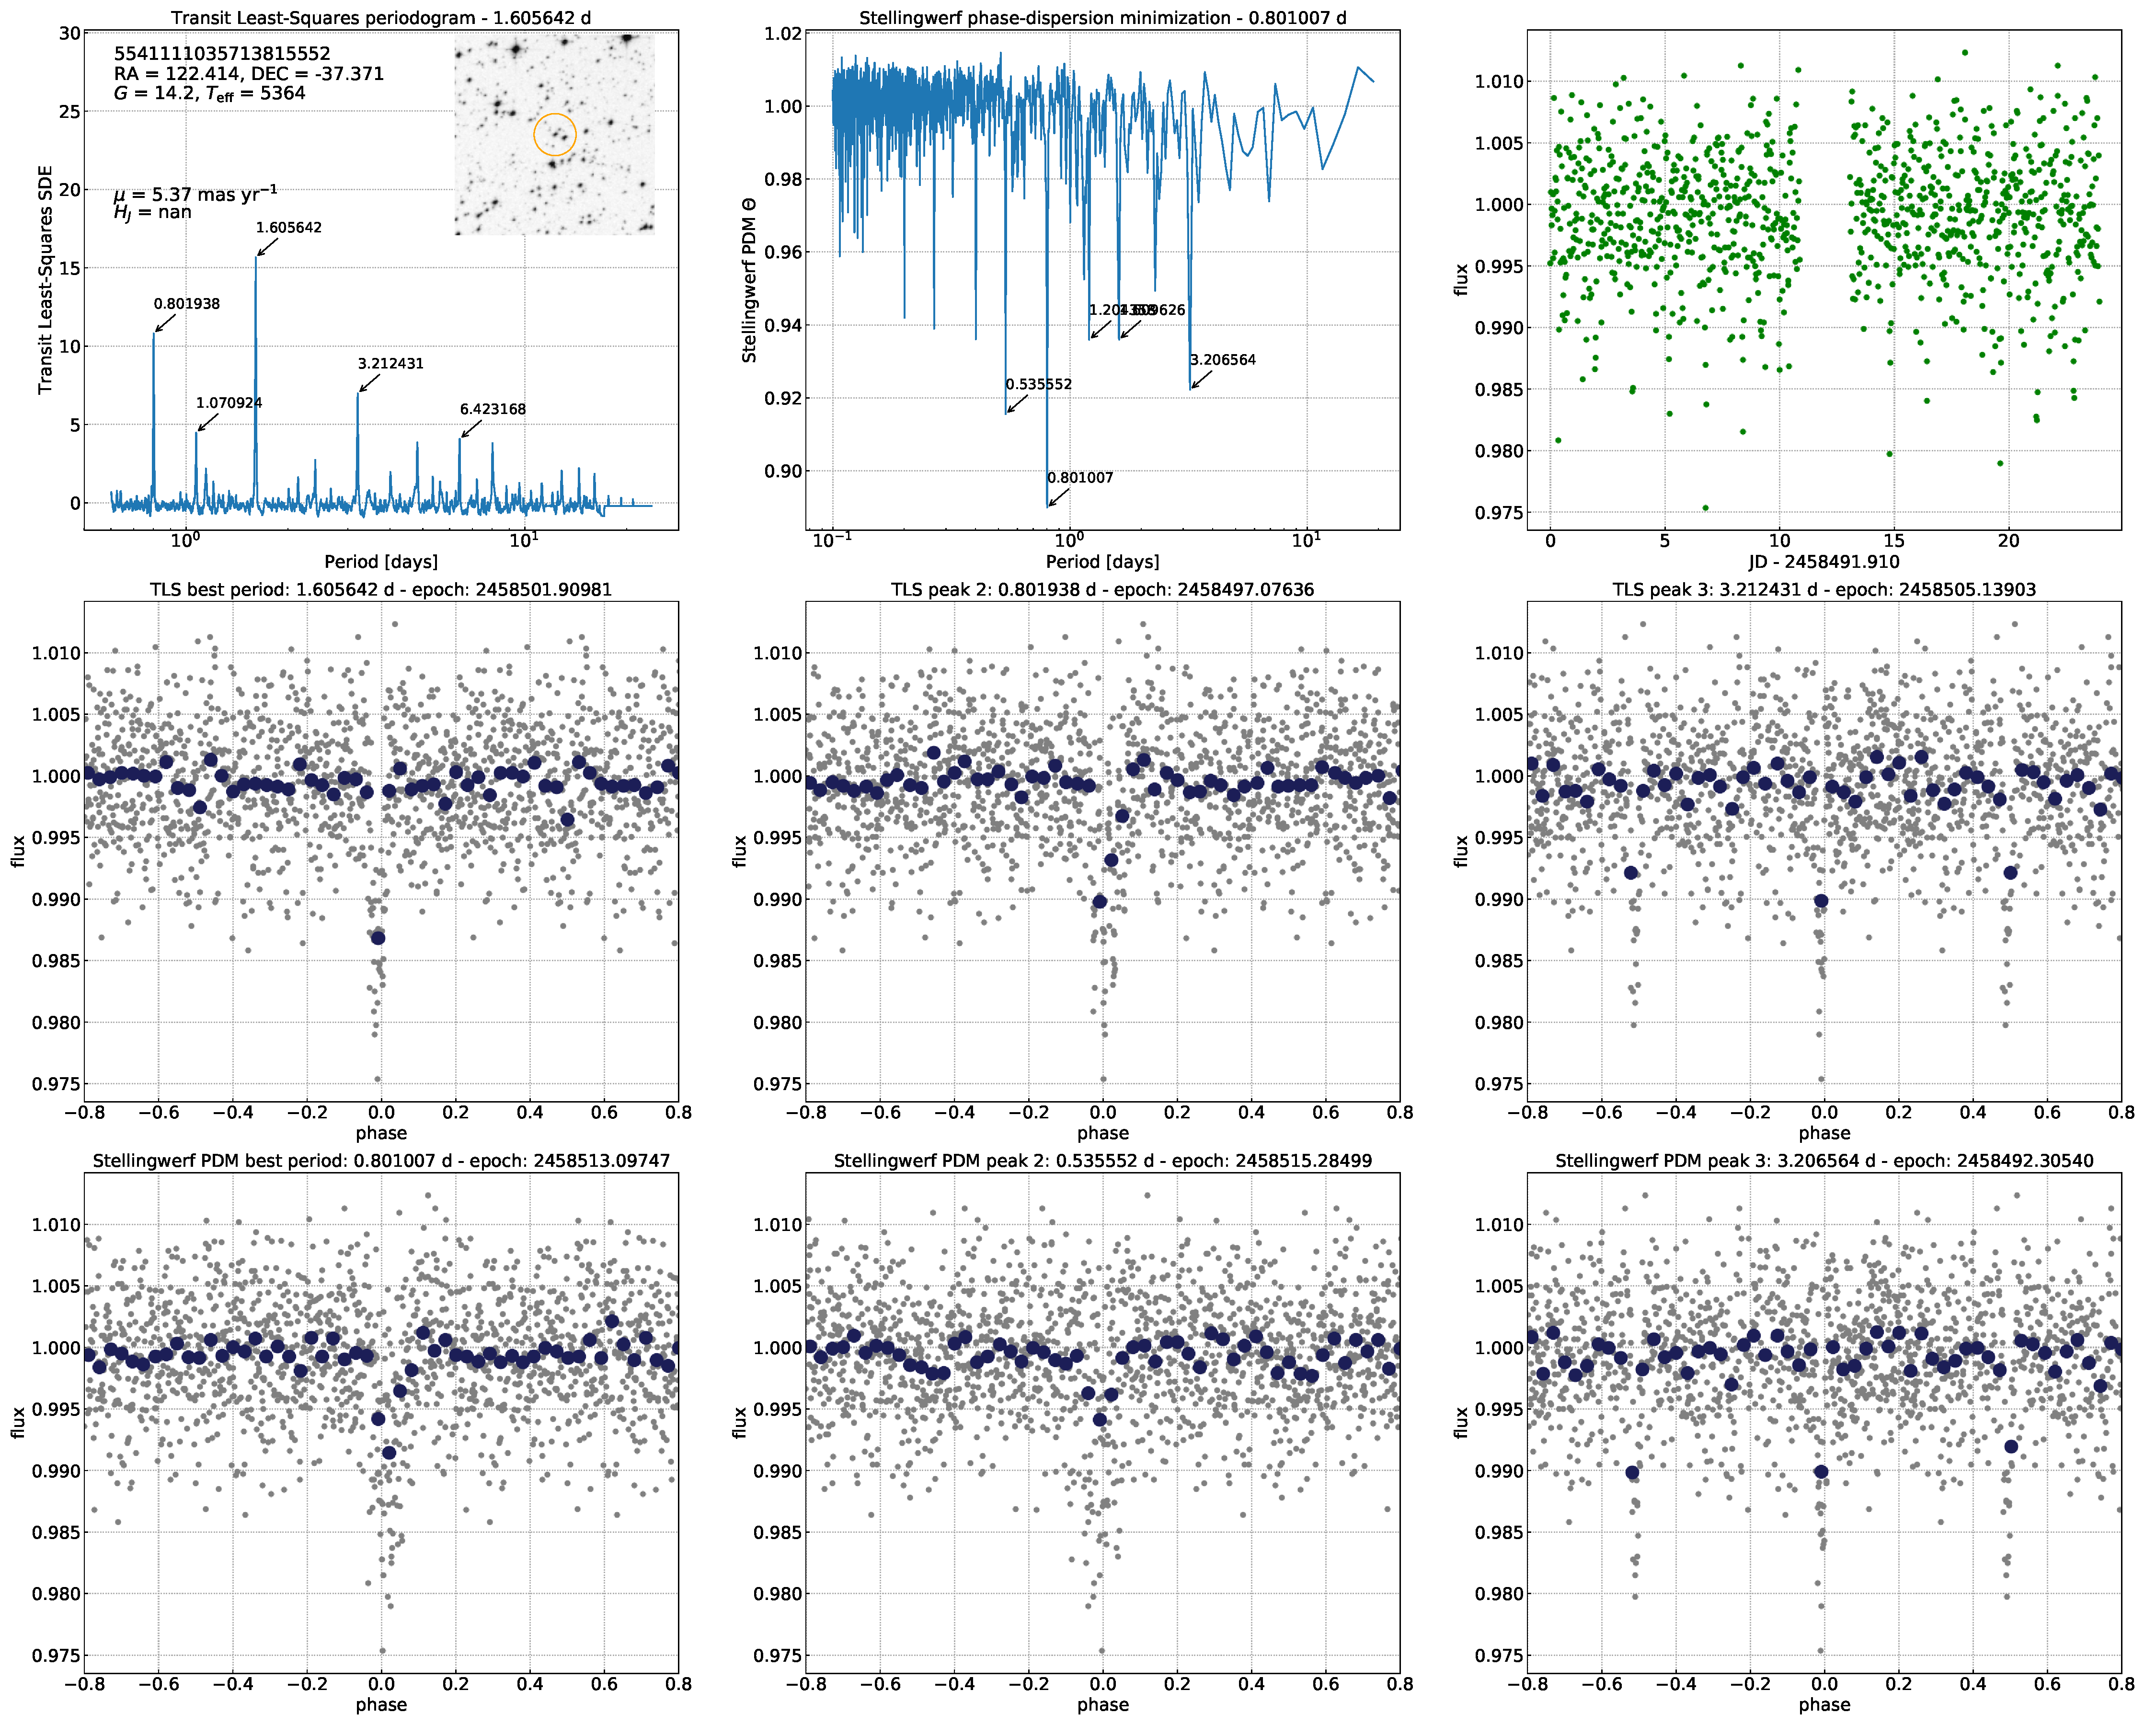
\includegraphics[width=0.98\textwidth]{gaiatwo0005541111035713815552-0007_page01.pdf}
	\end{center}
	\vspace{-0.5cm}
	\caption{
		{\bf Transit search summary.} Periodograms from TLS and 
		phase-dispersion minimization, as calculated 
		with \texttt{astrobase.periodbase}, are shown in the top left and top center 
		\citep{bhatti_astrobase_2018,hippke_TLS_2019,stellingwerf_period_1978}.
		The top three peaks from each 
		method are shown in the second and third rows; the raw light curve is in the 
		top-right. A small finder chart from DSS is inset to the top left, with
		the 1.5-pixel radius aperture used to extract the light curve in orange.
		\label{fig:pg1}
	}
\end{figure*}

\begin{figure*}[!h]
	\begin{center}
		\leavevmode
		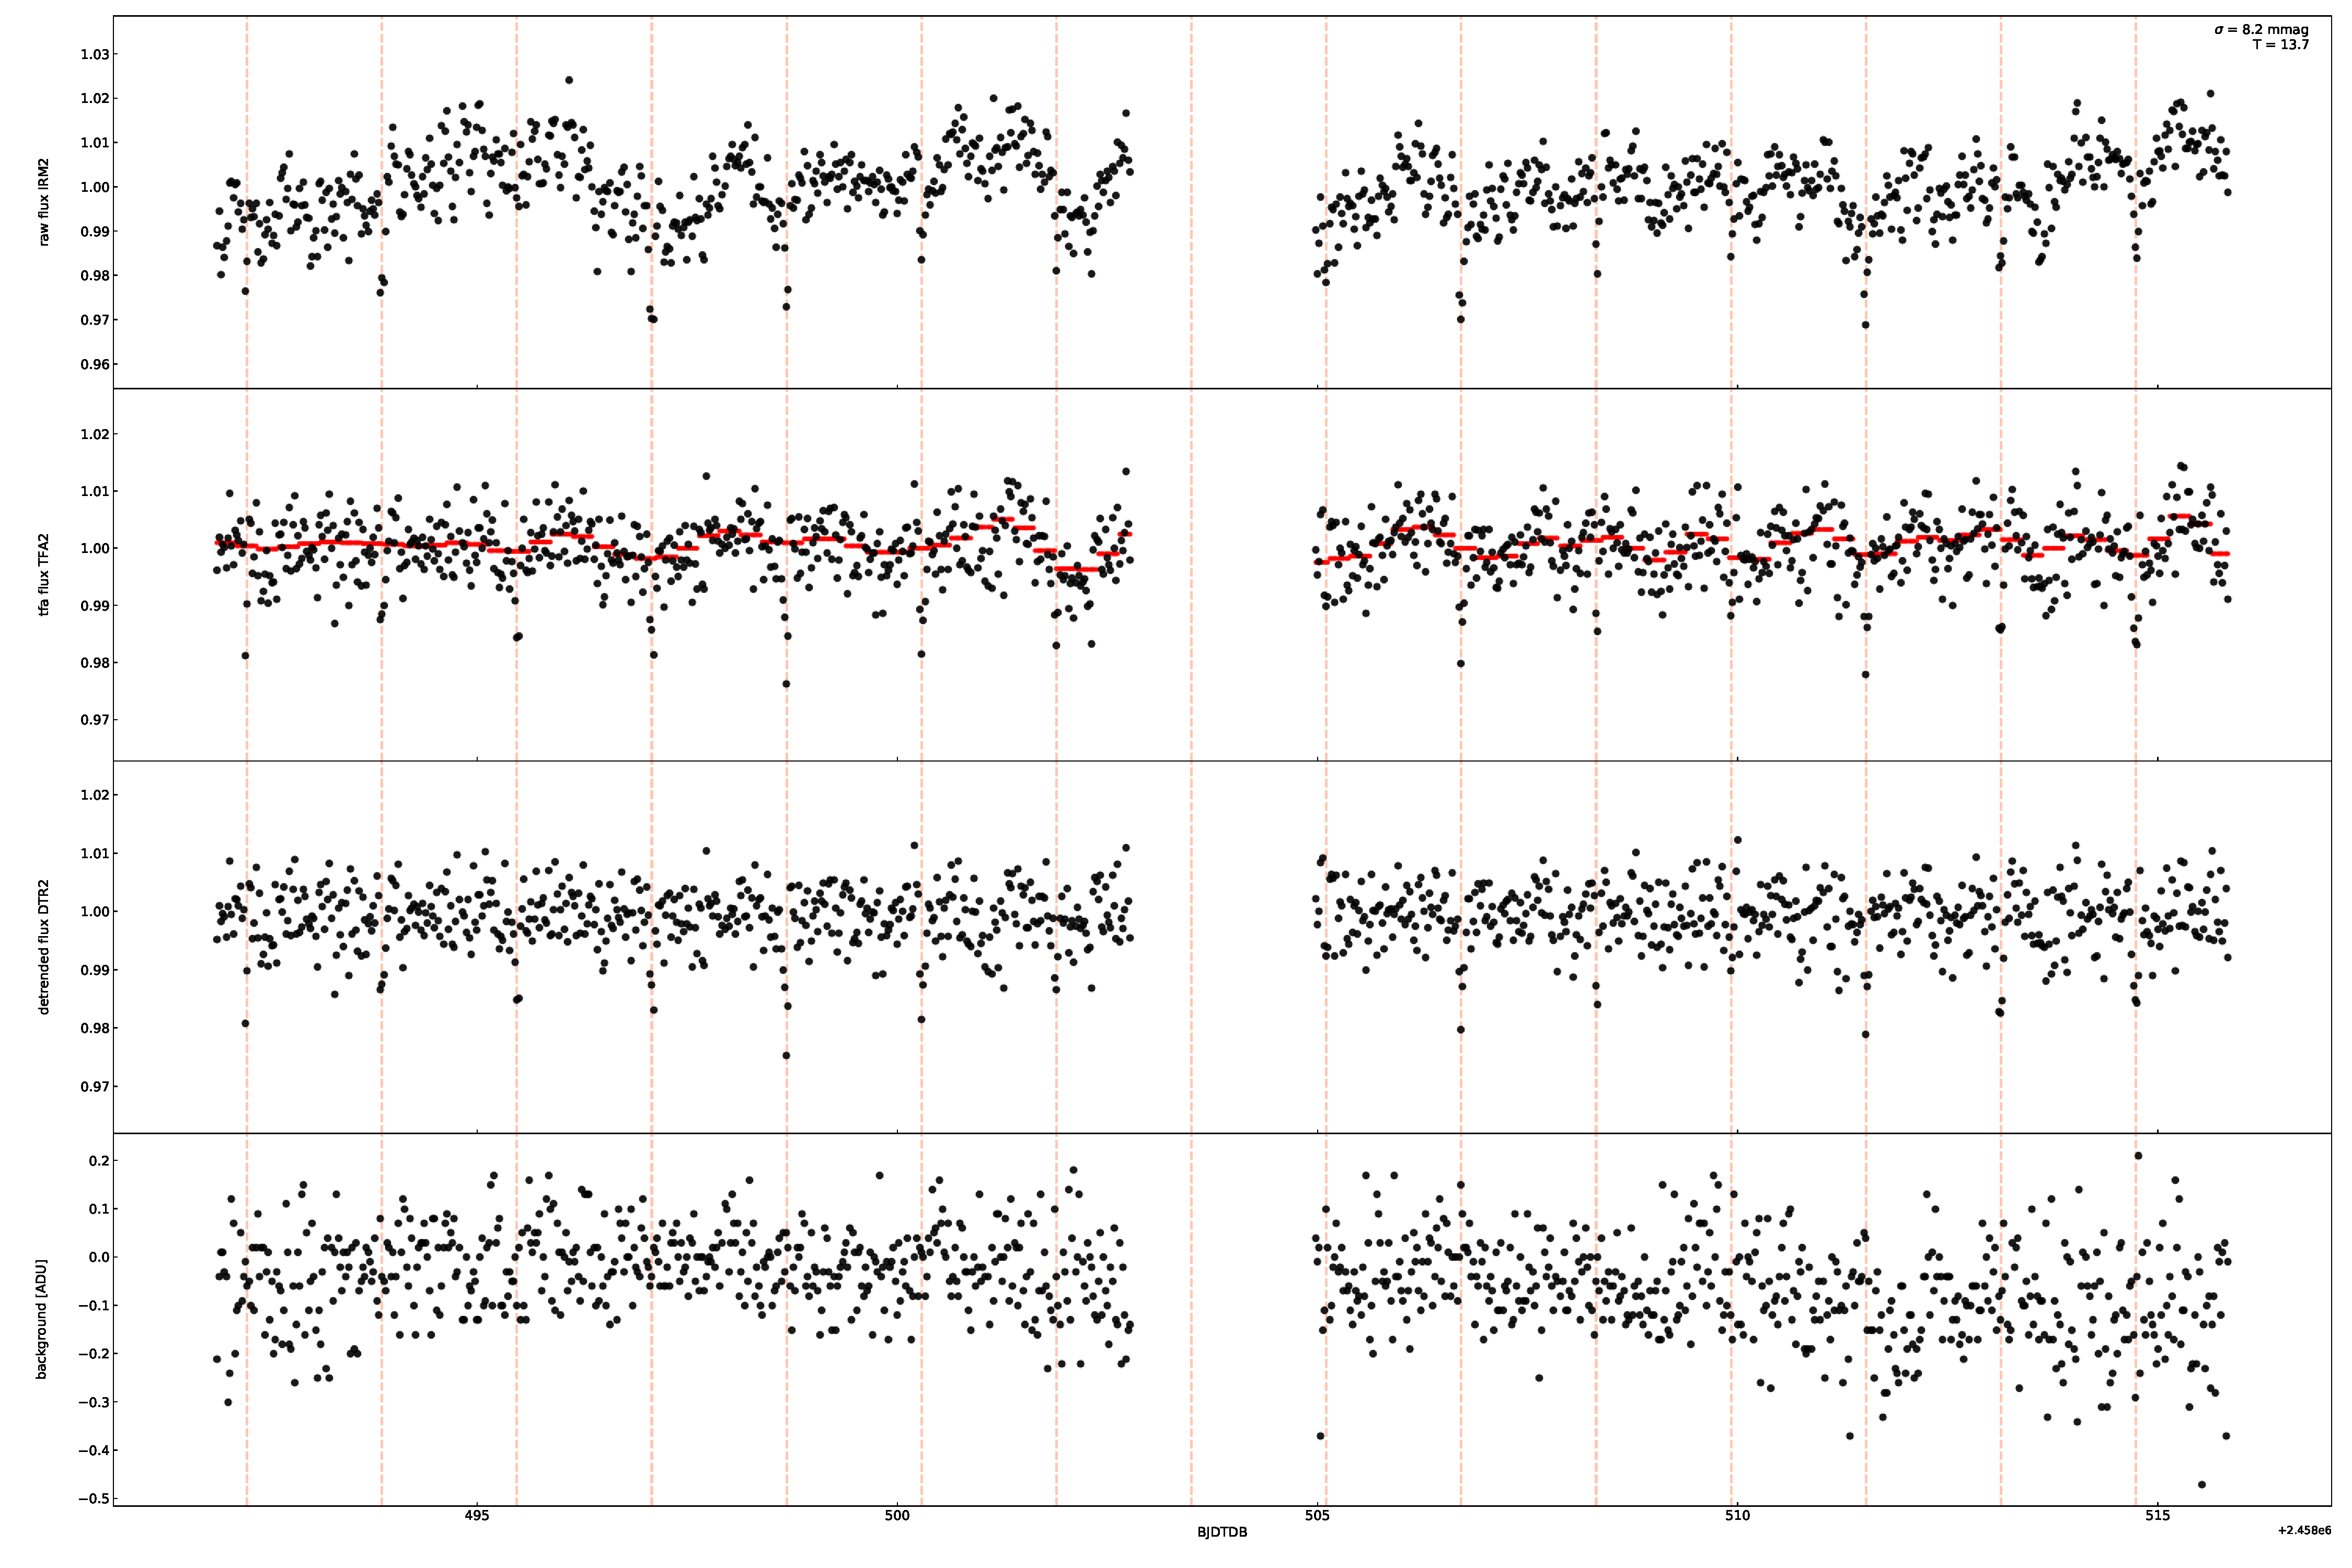
\includegraphics[width=0.98\textwidth]{gaiatwo0005541111035713815552-0007_page02.pdf}
	\end{center}
	\vspace{-0.5cm}
	\caption{
		{\bf Light curve diagnostics.} 
		Time-series of raw flux (\texttt{IRM2}),  TFA-detrended flux (\texttt{TF2}), stellar-variability
		detrended flux, and the background are shown as a function of
		barycentric Julian date.
		The overplotted dashed vertical lines are the ephemeris of the highest-power
		TLS peak from Figure~\ref{fig:pg1}.
		An important check is whether the flux dips are correlated with changes in the 
		background level -- in this case, they are not.
		The standard deviation and TESS magnitude are quoted in the upper right.
		The red line in the second from the top plot is the windowed 
		spline described in Section~\ref{subsec:ctois} -- in this case it is near its maximal
		frequency.
		\label{fig:pg2}
	}
\end{figure*}

\begin{figure*}[!h]
	\begin{center}
		\leavevmode
		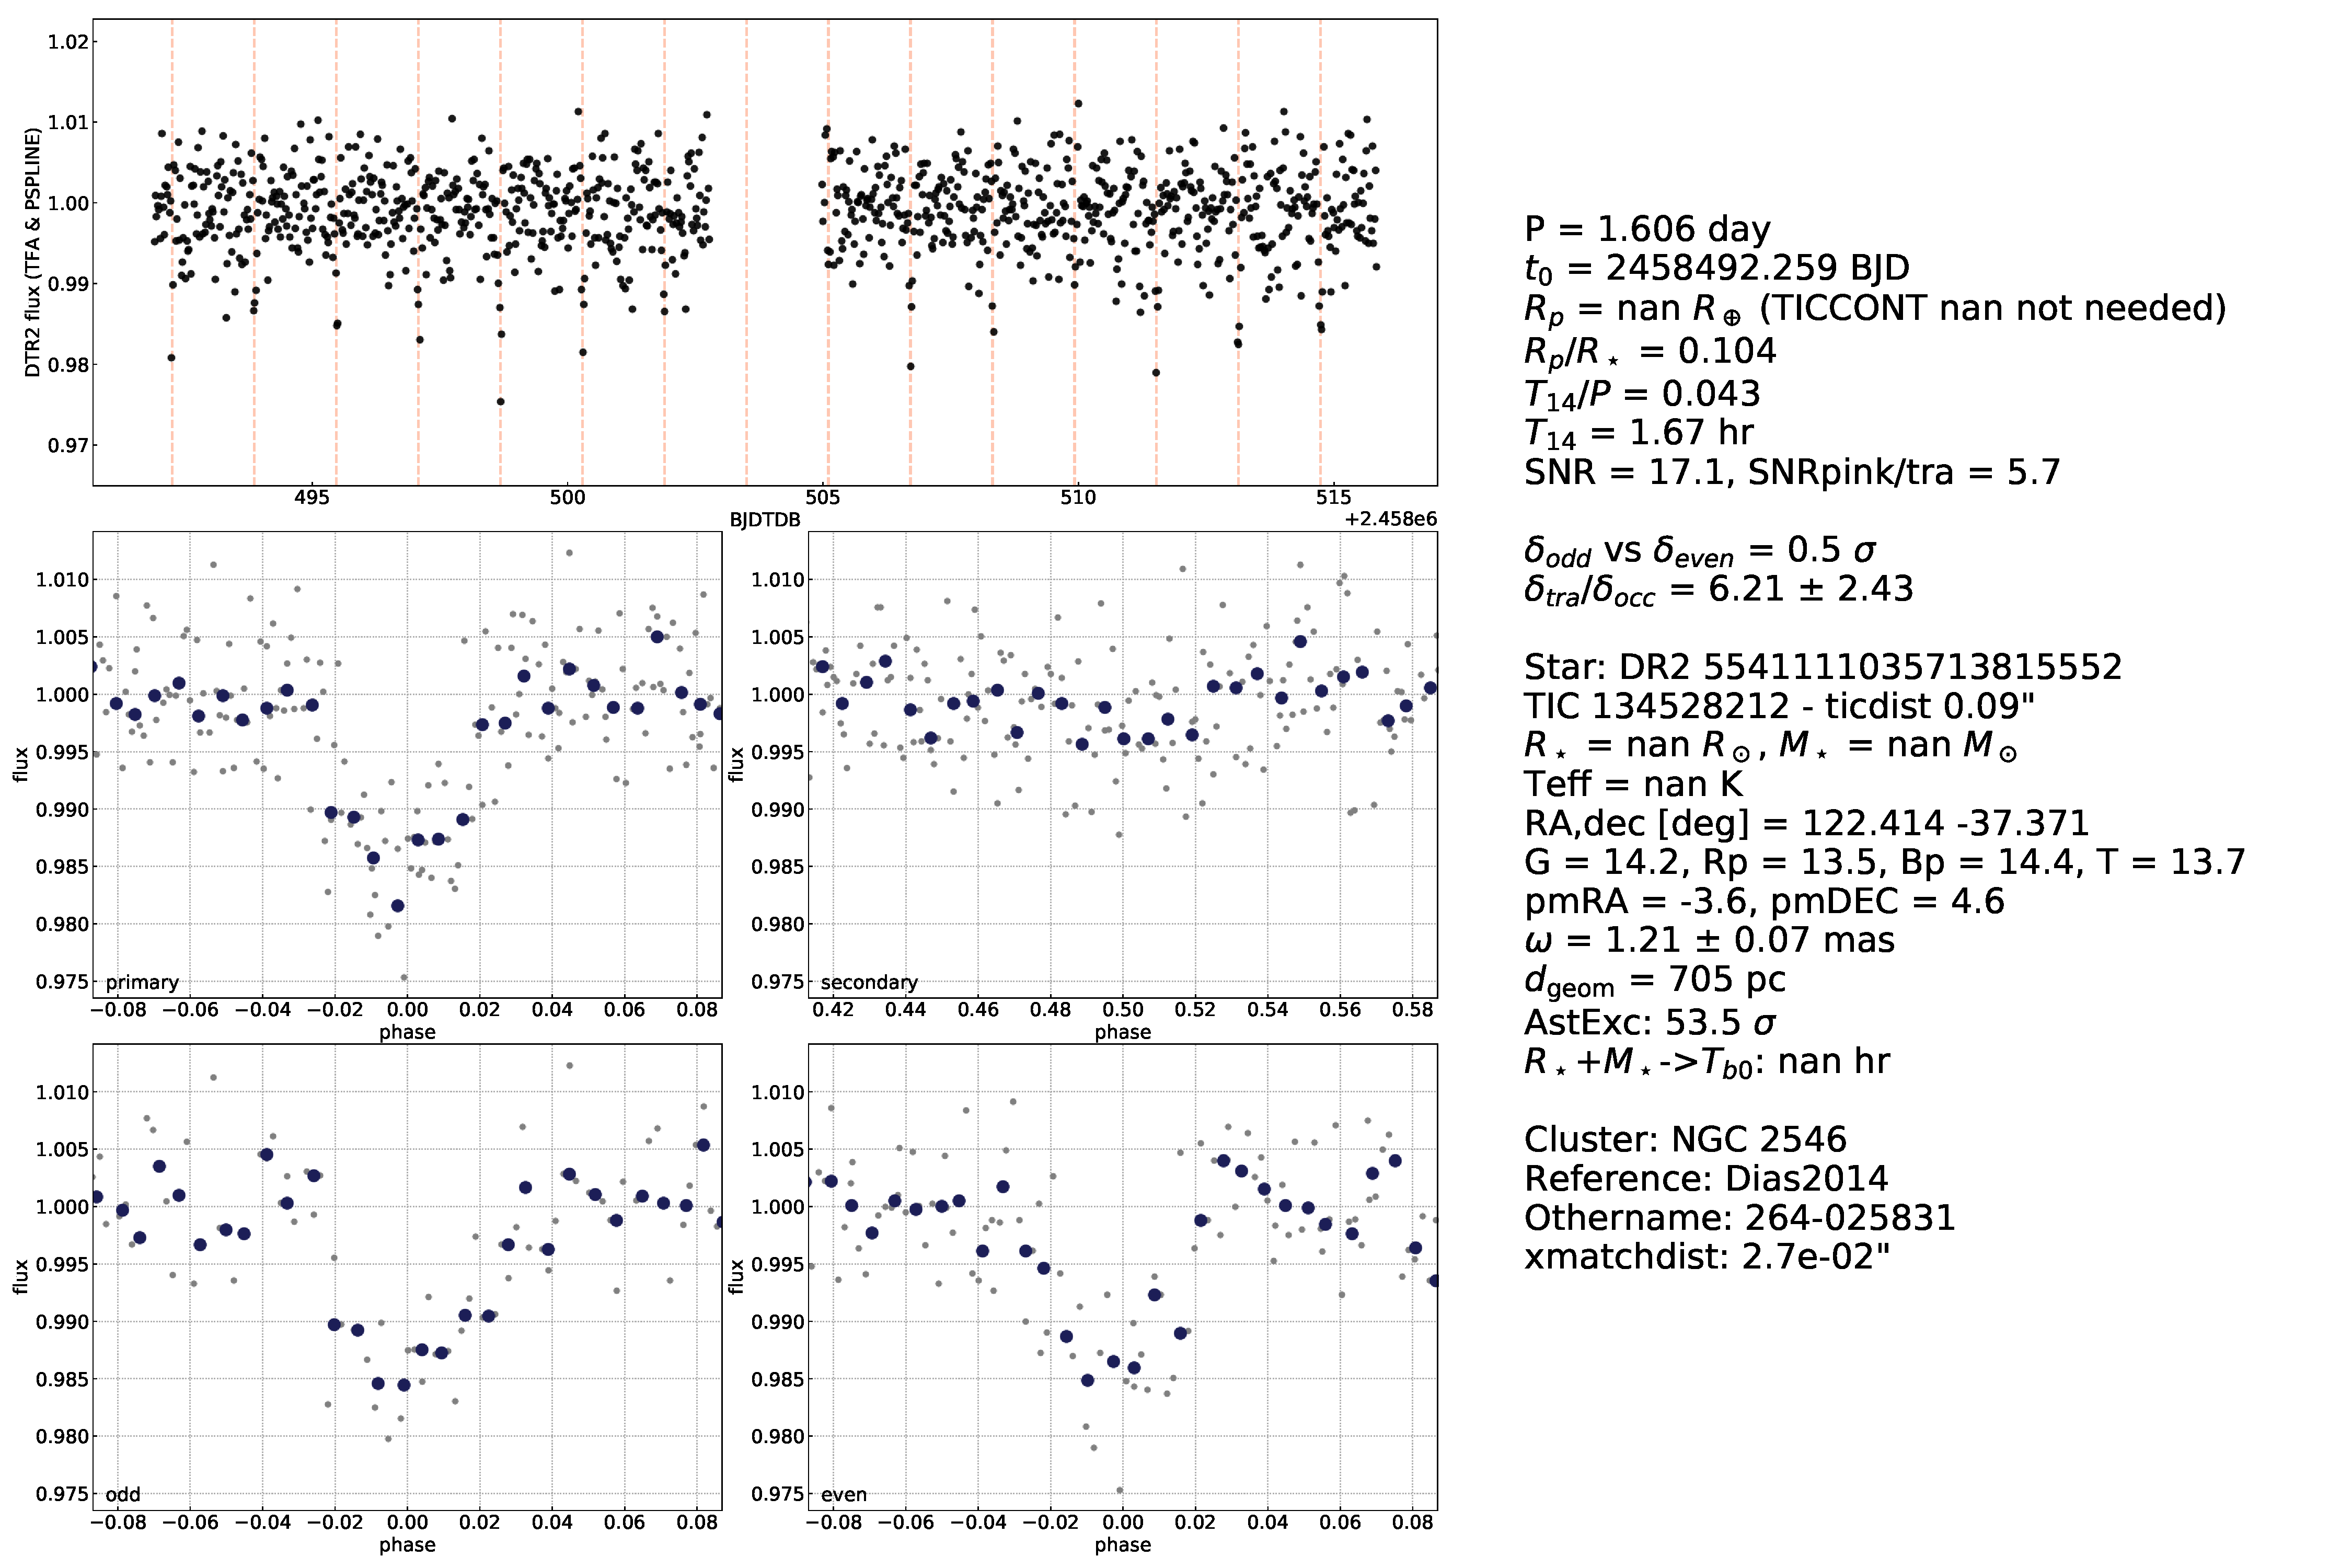
\includegraphics[width=0.98\textwidth]{gaiatwo0005541111035713815552-0007_page03.pdf}
	\end{center}
	\vspace{-0.5cm}
	\caption{
    {\bf Transit diagnostics.} The plots show the
    maximally-detrended light curve (top); the phase-folded light
    curve centered over $\pm3$ transit durations of the primary
    transit (middle left); the secondary eclipse (middle right); the
    odd-numbered transits (lower left); and the even-numbered transits
    (lower right).
    The stellar parameters ($T_{\rm eff}, R_\star, M_\star$) are taken from
    TICv8 when available \citep{stassun_TIC8_2019}.
    %Gaia-DR2 Apsis pipeline results when available
    %\citep{andrae_apsis_2018}.
    The first eight lines of text are parameters determined from the
    best-fitting TLS model.
    The one exception is the planet radius, which uses the stellar
    radius as noted above.
    The ``flux contamination'' (\texttt{TICCONT}) from neighboring
    stars is {\it never} taken into account, because transit depth
    dilution does not affect image subtraction analyses in the same
    manner as aperture-photometry reductions.
    To estimate the transit to occulation depth ratio, the
    phase-folded light curve is also coarsely fit via maximum
    likelihood by a sum of two gaussians.
    ``AstExc'' refers to the Gaia-DR2 astrometric excess, which can
    indicate hints of astrometric binarity in the system.
    ``$d_{\rm geom}$'' is the geometric distance from
    \citet{bailer-jones_distances_2018}.
    ``$R_\star + M_\star \rightarrow T_{b0}$'' gives the duration of a
    zero-eccentricity central transit based on the TICv8 stellar
    radius and mass if available. If the mass is not available, a
    stellar mass is interpolated from the
    \citet{pecaut_intrinsic_2013} table, under the assumption that the
    star is a dwarf.
    %\footnote{\url{http://www.pas.rochester.edu/~emamajek/EEM_dwarf_UBVIJHK_colors_Teff.txt}}.
		\label{fig:pg3}
	}
\end{figure*}

\begin{figure*}[!h]
	\begin{center}
		\leavevmode
		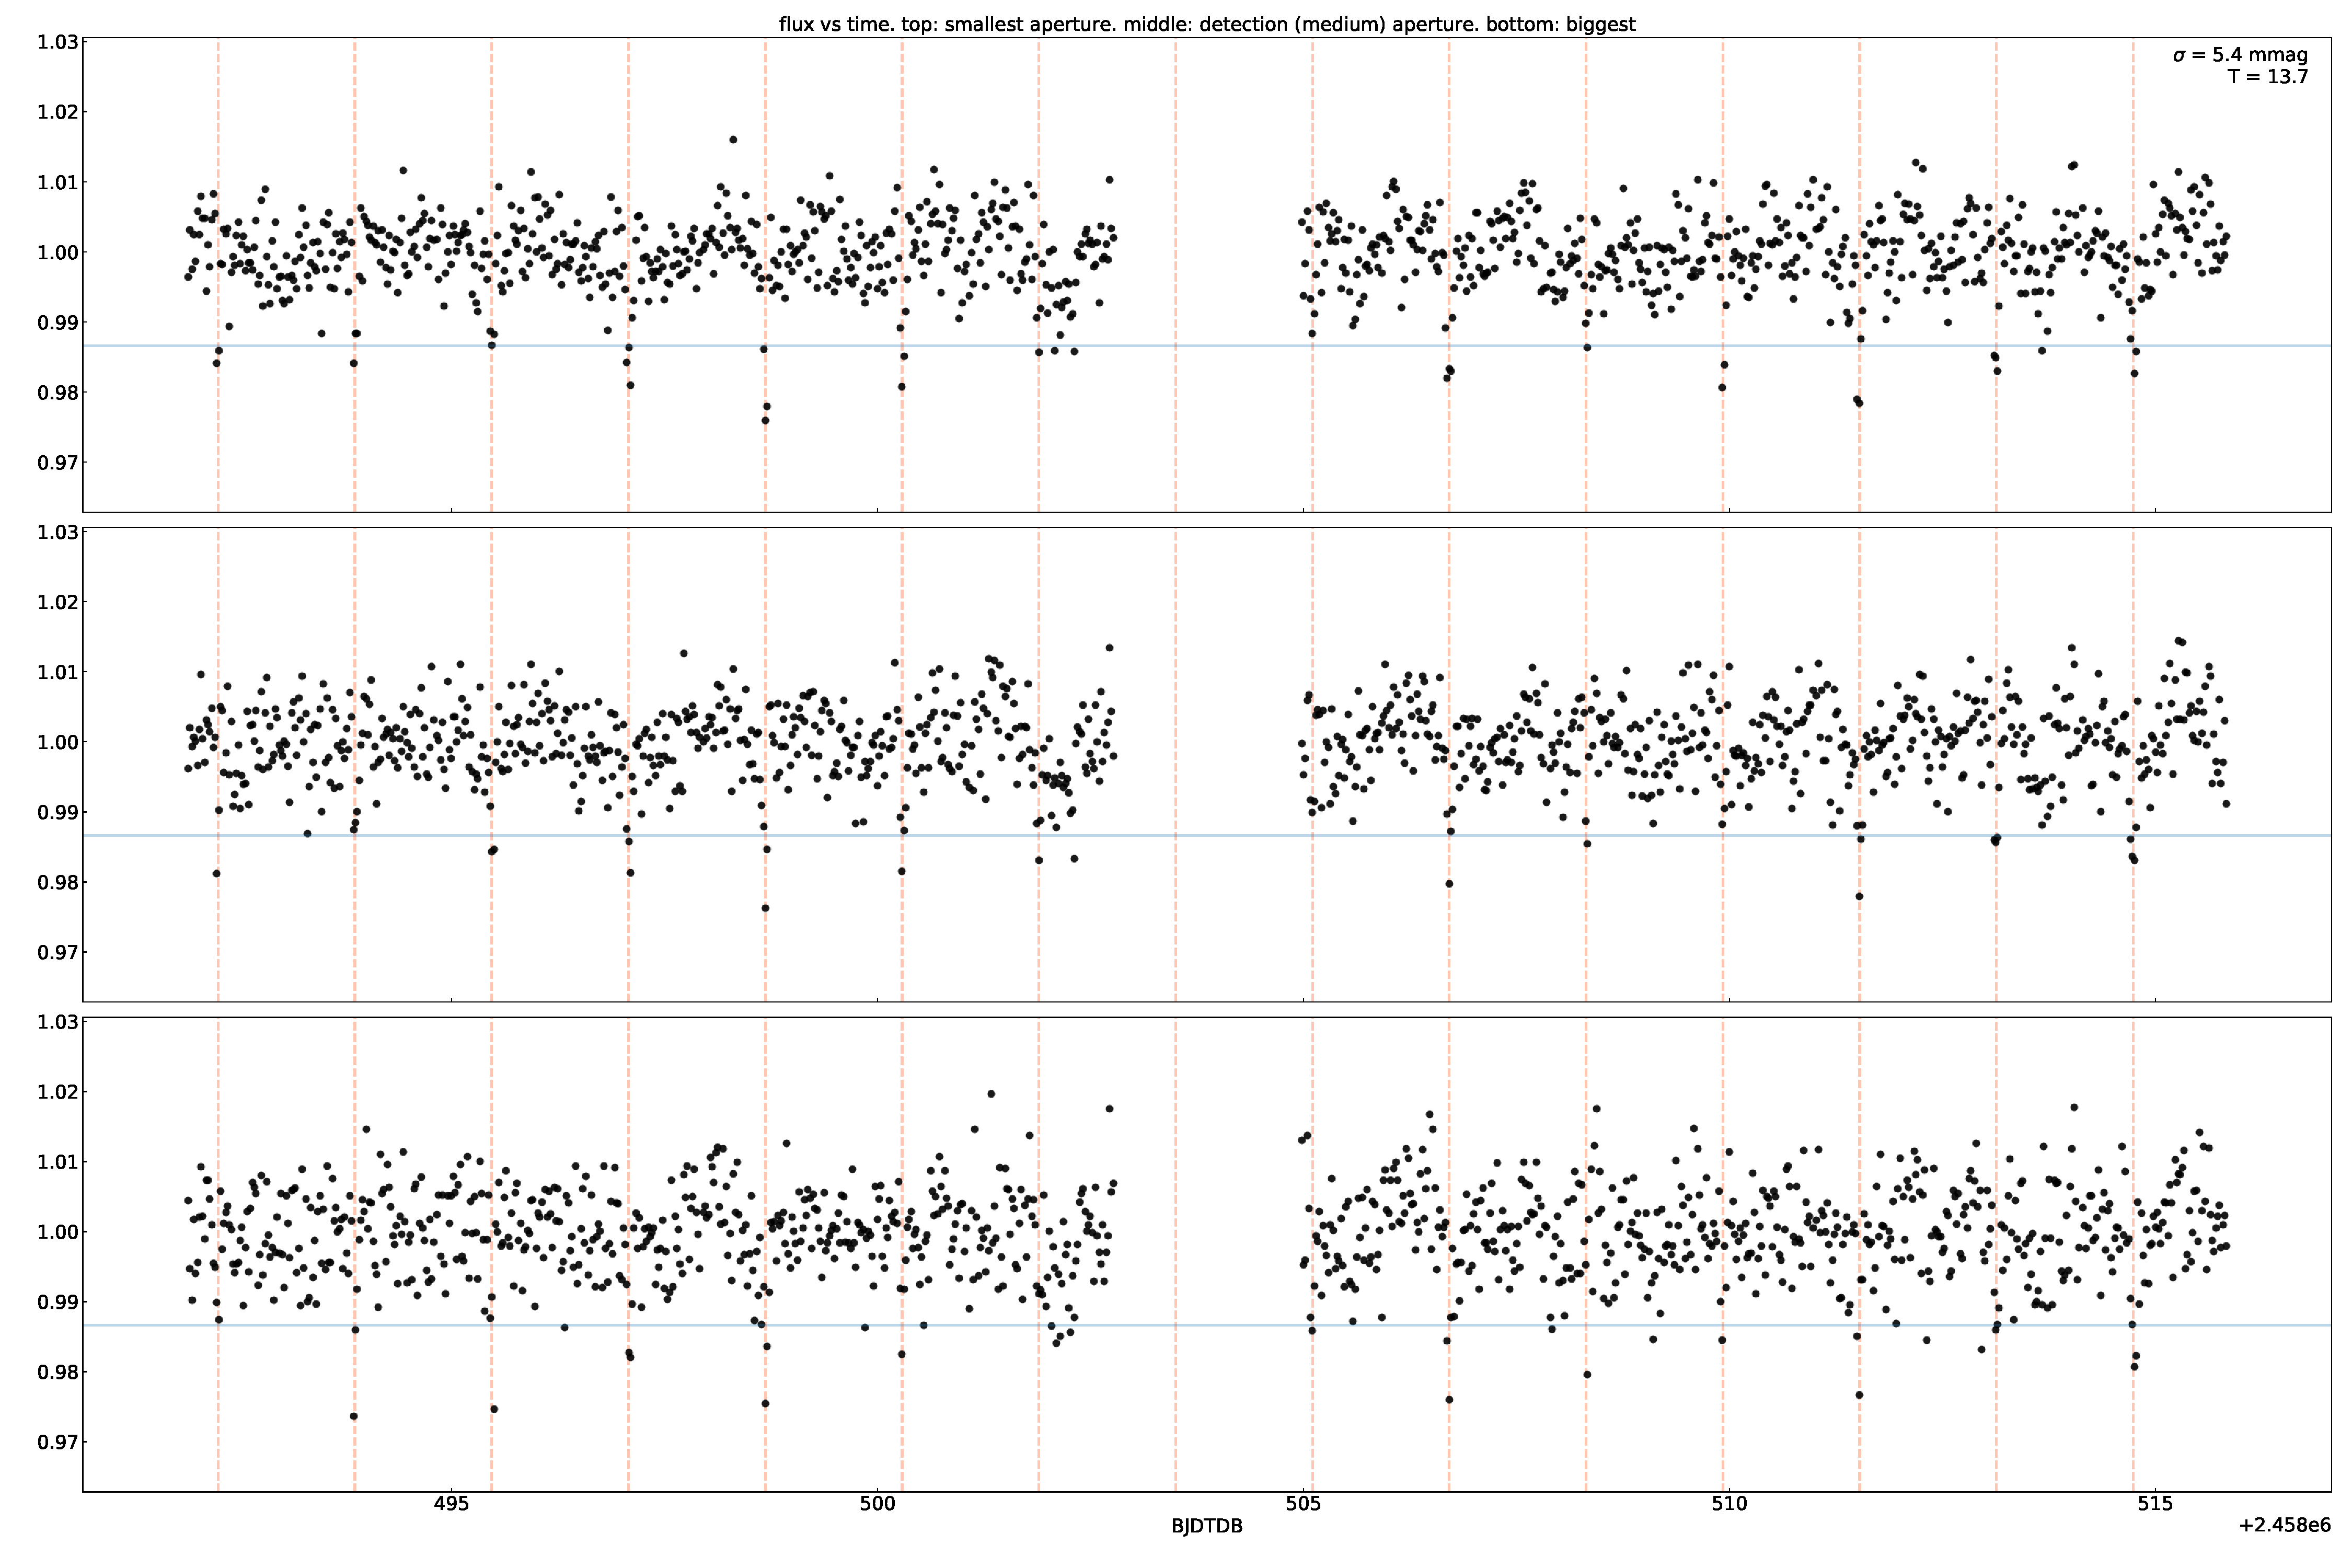
\includegraphics[width=0.98\textwidth]{gaiatwo0005541111035713815552-0007_page04.pdf}
	\end{center}
	\vspace{-0.5cm}
	\caption{
		{\bf Light curves for increasing aperture sizes.} 
		Apertures of radius 1, 1.5, and 2.25 pixels are shown from top to bottom.
		The blue line is the reference transit depth from the best-fitting TLS model.
		Any changes in depth with aperture size might indicate the need for a 
		detailed pixel-level analysis.
		\label{fig:pg4}
	}
\end{figure*}

\begin{figure*}[!h]
	\begin{center}
		\leavevmode
		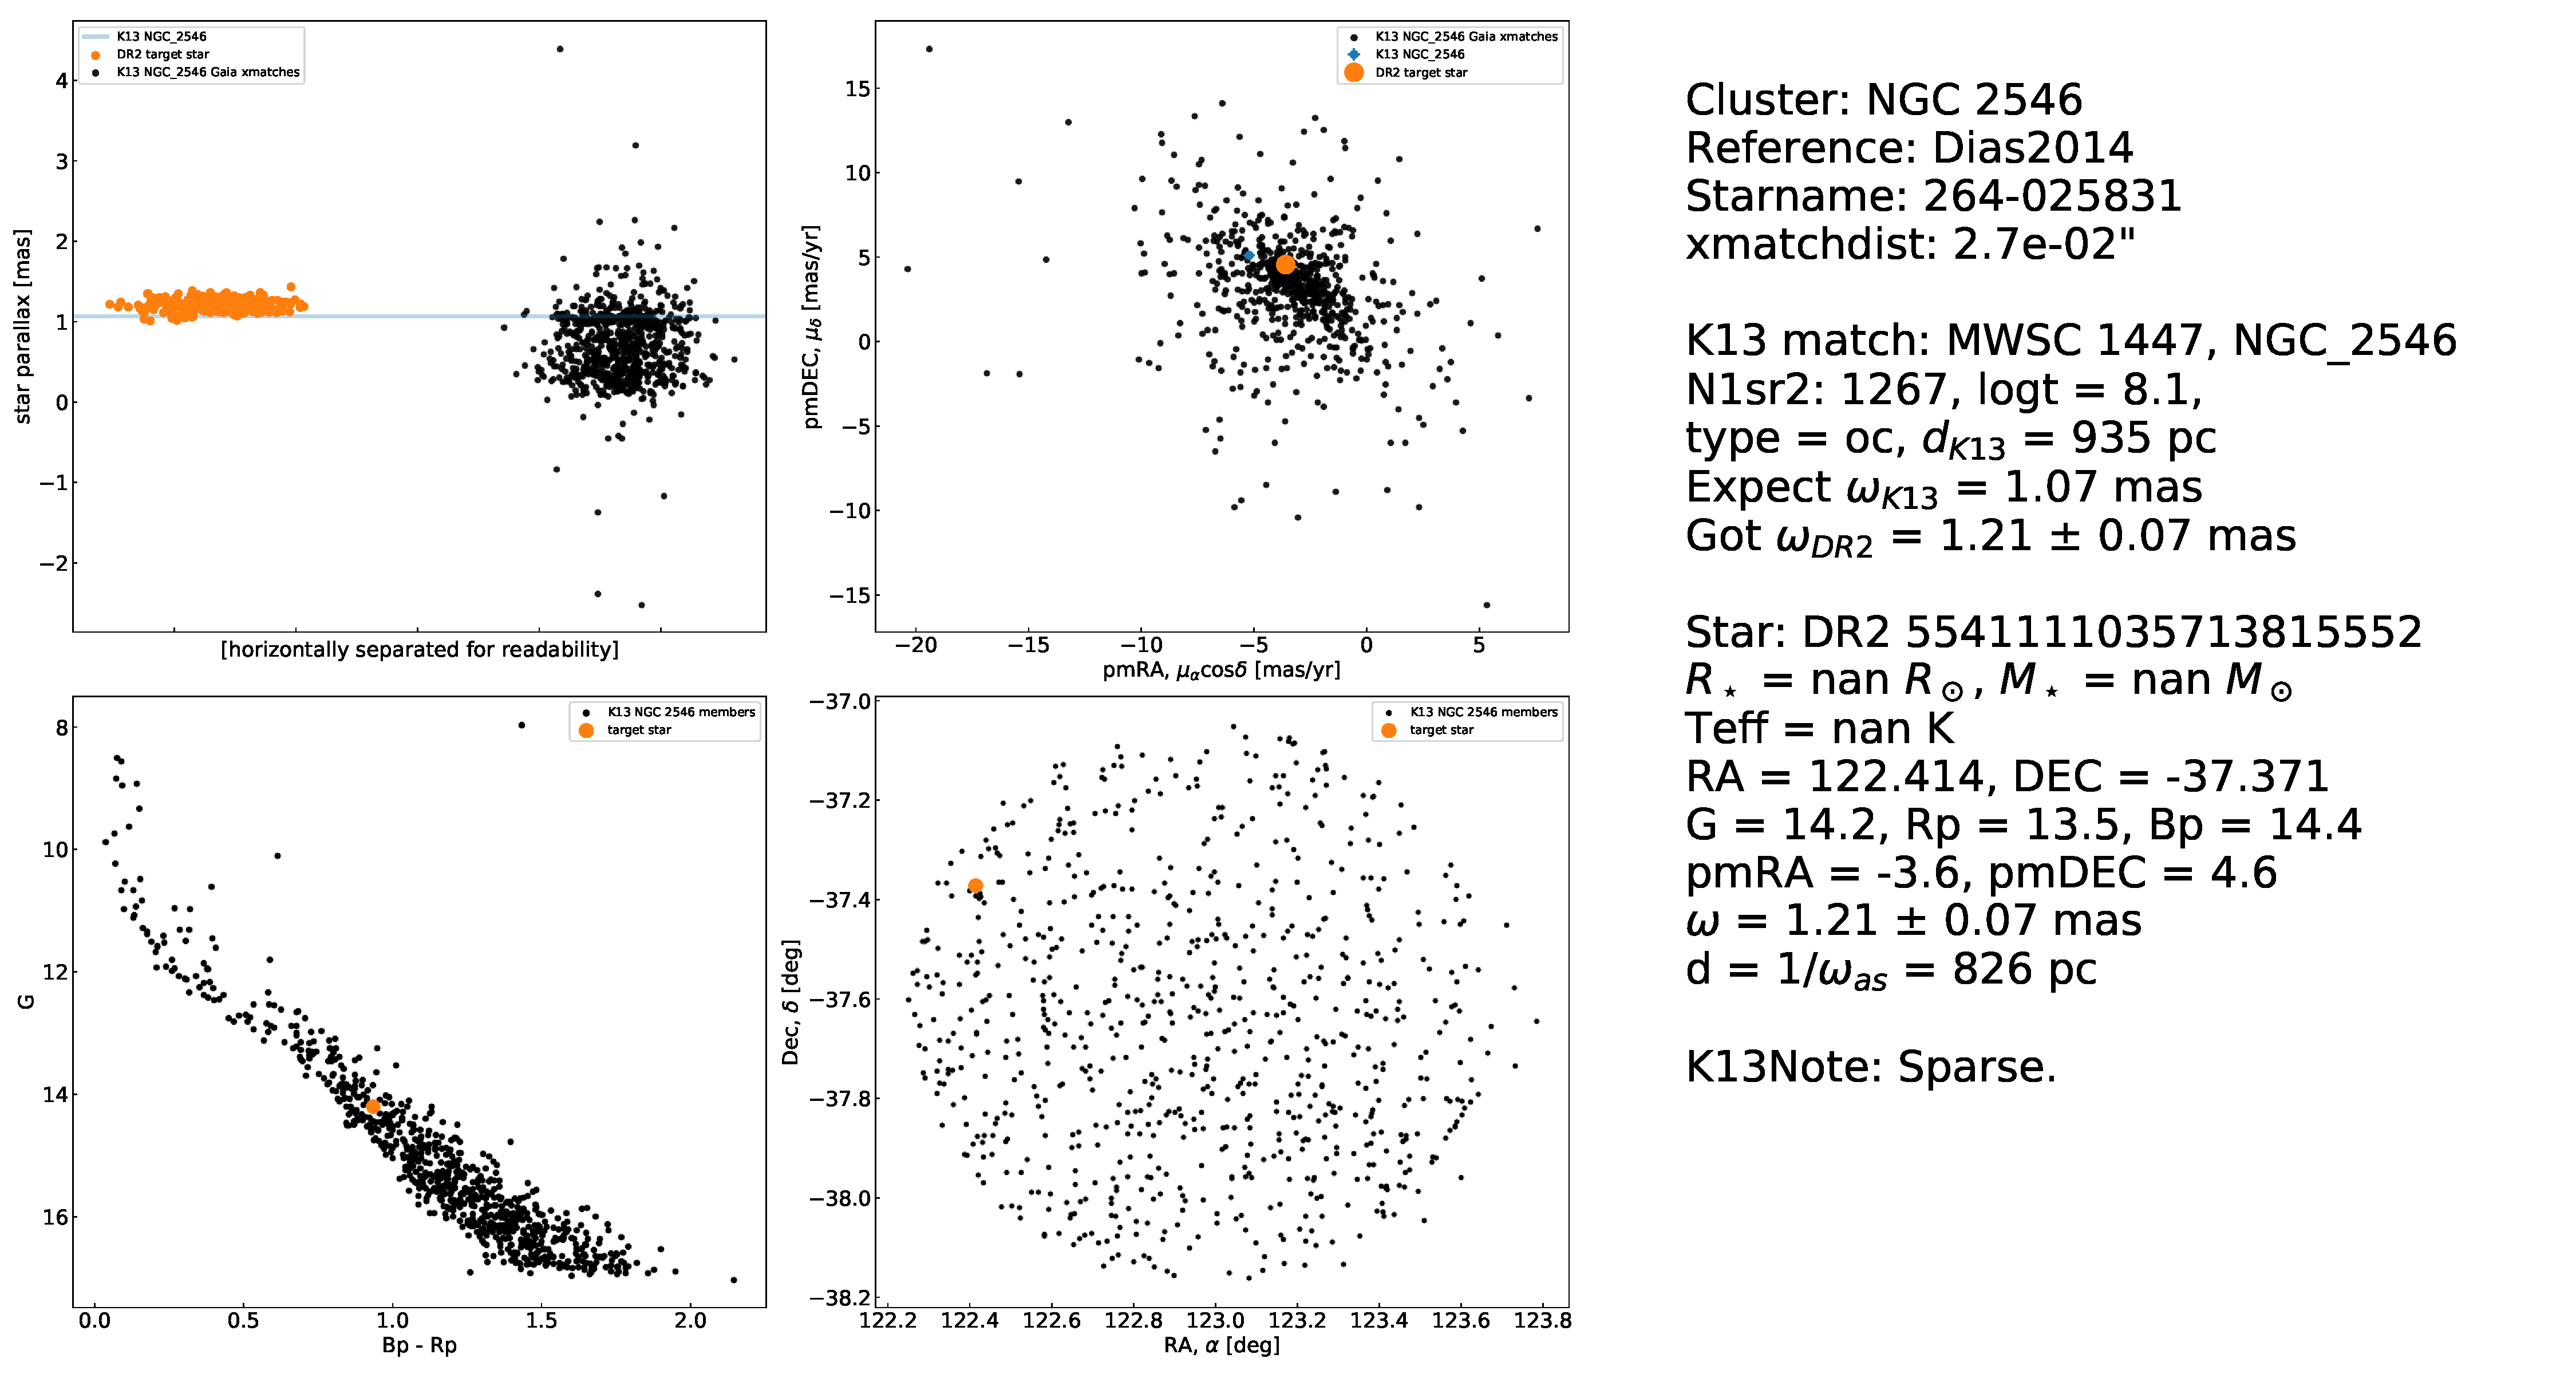
\includegraphics[width=0.98\textwidth]{gaiatwo0005541111035713815552-0007_page05.pdf}
	\end{center}
	\vspace{-0.5cm}
	\caption{
		{\bf Cluster membership assessment diagnostics.}
		The star was considered a candidate cluster member by the source(s) listed under
		``Reference'', in this case \citet{dias_proper_2014}.
		The name used in the Dias catalog in this case was \texttt{264-025831}, a
		UCAC-4 identifier, which can be back-referenced to find that \citet{dias_proper_2014}
		assigned this star a
		membership probability in NGC 2546 of 98\%.
		The base catalog for the plots is chiefly that of \citet{Kharchenko_et_al_2013},
		due to its homogeneous parameter determination procedure (particularly for age).
		If a match to the \citet{Kharchenko_et_al_2013} catalog is found, then the remaining
		plots are populated.
		Top-left shows the parallax, with orange points sampled from the Gaia-DR2
		posterior, black points the other cluster members in the Kharchenko catalog,
		and the blue line the claimed Kharchenko parallax for the cluster.
		A large number of field contaminants are visible in this case.
		Top-right are the Gaia proper motions, where against black points are cluster
		members from Kharchenko, and the orange is the target star.
    Bottom-left is the color-magnitude diagram, and bottom-right are
    the on-sky positions.  In the text,
		\texttt{N1sr2} is the number of $1\sigma$ cluster members reported
		by \citet{Kharchenko_et_al_2013} within the cluster angular radius;
		$\log t$ is the base-10 logarithm of the age in years;
		\texttt{type} matches the type codes provided by
    \citet{Kharchenko_et_al_2013};
    \texttt{K13Note} gives the description of the cluster from
    \citet{Kharchenko_et_al_2013}, if available.
		\label{fig:pg5}
	}
\end{figure*}

\begin{figure*}[!h]
	\begin{center}
		\leavevmode
		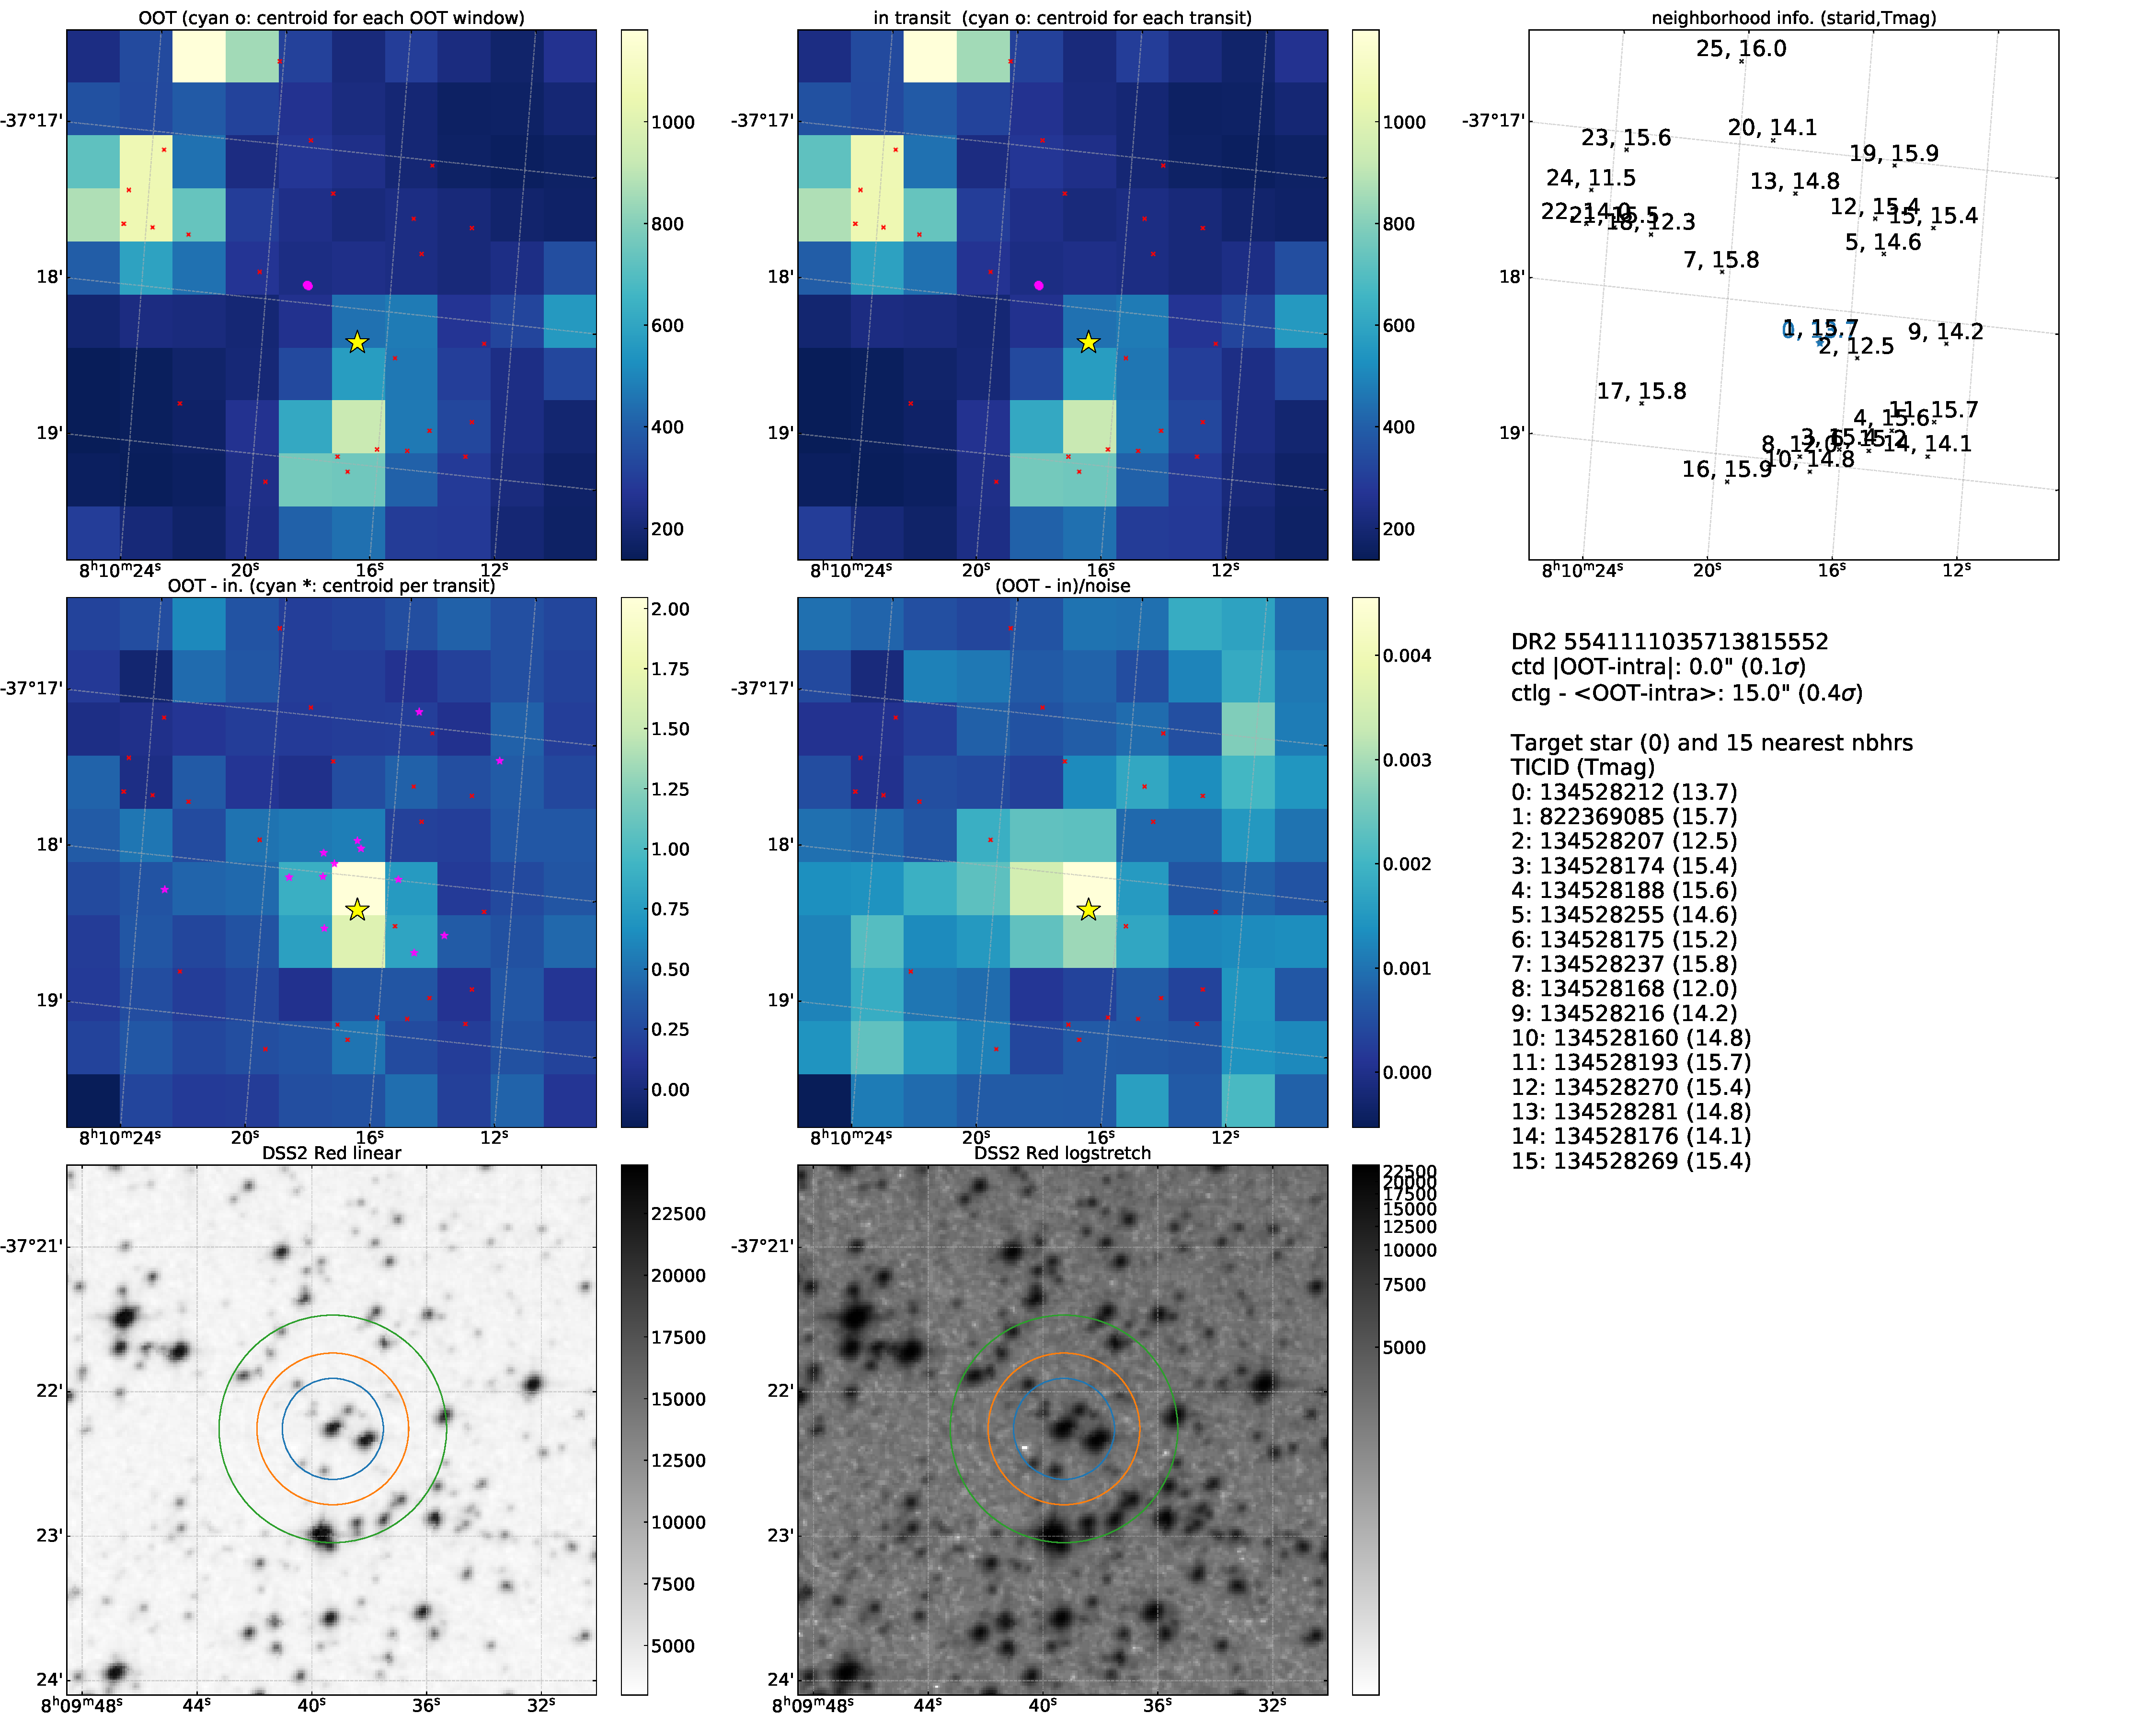
\includegraphics[width=0.98\textwidth]{gaiatwo0005541111035713815552-0007_page06.pdf}
	\end{center}
	\vspace{-0.5cm}
	\caption{
		{\bf Imaging variability diagnostics.} 
		This page is intended to help diagnose which stars are producing the observed
		variability.
		Top-left and top-center are the mean out-of-transit (OOT) and mean in-transit 
		calibrated images (separate from any of our image-subtraction analysis).
		The OOT images are based on the same number of exposures as the in-transit images
		and split evenly before and after each transit \citep[following][]{bryson_identification_2013,kostov_l9859_2019}.
		The yellow star is the target; cyan dots are the flux-weighted centroid of the entire
		image for each transit event; small red crosses are WCS-projected locations of neighbor stars.
		Middle-left is the most important sub-panel: the difference between
		the OOT and in-transit mean images.
		If the variability shown in background map (units: ADU) is off-target, the
		transit is typically not from the target star.
		Middle-center is the same, normalized by the uncertainty map.
		Lower left and lower center show the DSS field in linear and log scales
		at roughly the same pixel scale as the TESS image,
		with the 1, 1.5, and 2.25 pixel-radius apertures in blue, orange, and green respectively.
		The brightness of neighborhood stars is given on the far right.
		Note the slight rotation difference between DSS and TESS images;
		DSS images are aligned north-up, east-left; TESS images are oriented as closely as
		possible to this system without actually performing the rotation.
		\label{fig:pg6}
	}
\end{figure*}

\end{document}

